%% bare_jrnl_compsoc.tex
%% V1.4b
%% 2015/08/26
%% by Michael Shell
%% See:
%% http://www.michaelshell.org/
%% for current contact information.
%%
%% This is a skeleton file demonstrating the use of IEEEtran.cls
%% (requires IEEEtran.cls version 1.8b or later) with an IEEE
%% Computer Society journal paper.
%%
%% Support sites:
%% http://www.michaelshell.org/tex/ieeetran/
%% http://www.ctan.org/pkg/ieeetran
%% and
%% http://www.ieee.org/

%%*************************************************************************
%% Legal Notice:
%% This code is offered as-is without any warranty either expressed or
%% implied; without even the implied warranty of MERCHANTABILITY or
%% FITNESS FOR A PARTICULAR PURPOSE! 
%% User assumes all risk.
%% In no event shall the IEEE or any contributor to this code be liable for
%% any damages or losses, including, but not limited to, incidental,
%% consequential, or any other damages, resulting from the use or misuse
%% of any information contained here.
%%
%% All comments are the opinions of their respective authors and are not
%% necessarily endorsed by the IEEE.
%%
%% This work is distributed under the LaTeX Project Public License (LPPL)
%% ( http://www.latex-project.org/ ) version 1.3, and may be freely used,
%% distributed and modified. A copy of the LPPL, version 1.3, is included
%% in the base LaTeX documentation of all distributions of LaTeX released
%% 2003/12/01 or later.
%% Retain all contribution notices and credits.
%% ** Modified files should be clearly indicated as such, including  **
%% ** renaming them and changing author support contact information. **
%%*************************************************************************


% *** Authors should verify (and, if needed, correct) their LaTeX system  ***
% *** with the testflow diagnostic prior to trusting their LaTeX platform ***
% *** with production work. The IEEE's font choices and paper sizes can   ***
% *** trigger bugs that do not appear when using other class files.       ***                          ***
% The testflow support page is at:
% http://www.michaelshell.org/tex/testflow/


\documentclass[10pt,journal,compsoc]{IEEEtran}

\usepackage{afterpage}
\usepackage{stfloats}
\usepackage{cuted}
\usepackage{caption}
\usepackage{graphicx}
\usepackage{adjustbox}
\usepackage{amsmath}
\usepackage{amssymb}
\usepackage{enumitem}
\usepackage{booktabs}
\usepackage{multirow}
\usepackage{url}
\usepackage{subcaption}
\usepackage{array}
\usepackage{tikz}
\usetikzlibrary{shapes,arrows.meta,positioning,fit,calc}
\usepackage[edges]{forest}
\usepackage{ragged2e}
\usepackage[table]{xcolor}
\definecolor{mygreen}{rgb}{0.0, 0.5, 0.0}
\usepackage{capt-of}

%
% If IEEEtran.cls has not been installed into the LaTeX system files,
% manually specify the path to it like:
% \documentclass[10pt,journal,compsoc]{../sty/IEEEtran}

% Some very useful LaTeX packages include:
% (uncomment the ones you want to load)


% *** MISC UTILITY PACKAGES ***
%
%\usepackage{ifpdf}
% Heiko Oberdiek's ifpdf.sty is very useful if you need conditional
% compilation based on whether the output is pdf or dvi.
% usage:
% \ifpdf
%   % pdf code
% \else
%   % dvi code
% \fi
% The latest version of ifpdf.sty can be obtained from:
% http://www.ctan.org/pkg/ifpdf
% Also, note that IEEEtran.cls V1.7 and later provides a builtin
% \ifCLASSINFOpdf conditional that works the same way.
% When switching from latex to pdflatex and vice-versa, the compiler may
% have to be run twice to clear warning/error messages.

% *** CITATION PACKAGES ***
%
\ifCLASSOPTIONcompsoc
  % IEEE Computer Society needs nocompress option
  % requires cite.sty v4.0 or later (November 2003)
  \usepackage[nocompress]{cite}
\else
  % normal IEEE
  \usepackage{cite}
\fi
% cite.sty was written by Donald Arseneau
% V1.6 and later of IEEEtran pre-defines the format of the cite.sty package
% \cite{} output to follow that of the IEEE. Loading the cite package will
% result in citation numbers being automatically sorted and properly
% "compressed/ranged". e.g., [1], [9], [2], [7], [5], [6] without using
% cite.sty will become [1], [2], [5]--[7], [9] using cite.sty. cite.sty's
% \cite will automatically add leading space, if needed. Use cite.sty's
% noadjust option (cite.sty V3.8 and later) if you want to turn this off
% such as if a citation ever needs to be enclosed in parenthesis.
% cite.sty is already installed on most LaTeX systems. Be sure and use
% version 5.0 (2009-03-20) and later if using hyperref.sty.
% The latest version can be obtained at:
% http://www.ctan.org/pkg/cite
% The documentation is contained in the cite.sty file itself.
%
% Note that some packages require special options to format as the Computer
% Society requires. In particular, Computer Society  papers do not use
% compressed citation ranges as is done in typical IEEE papers
% (e.g., [1]-[4]). Instead, they list every citation separately in order
% (e.g., [1], [2], [3], [4]). To get the latter we need to load the cite
% package with the nocompress option which is supported by cite.sty v4.0
% and later. Note also the use of a CLASSOPTION conditional provided by
% IEEEtran.cls V1.7 and later.

% *** GRAPHICS RELATED PACKAGES ***
%
\ifCLASSINFOpdf
  % \usepackage[pdftex]{graphicx}
  % declare the path(s) where your graphic files are
  % \graphicspath{{../pdf/}{../jpeg/}}
  % and their extensions so you won't have to specify these with
  % every instance of \includegraphics
  % \DeclareGraphicsExtensions{.pdf,.jpeg,.png}
\else
  % or other class option (dvipsone, dvipdf, if not using dvips). graphicx
  % will default to the driver specified in the system graphics.cfg if no
  % driver is specified.
  % \usepackage[dvips]{graphicx}
  % declare the path(s) where your graphic files are
  % \graphicspath{{../eps/}}
  % and their extensions so you won't have to specify these with
  % every instance of \includegraphics
  % \DeclareGraphicsExtensions{.eps}
\fi
% graphicx was written by David Carlisle and Sebastian Rahtz. It is
% required if you want graphics, photos, etc. graphicx.sty is already
% installed on most LaTeX systems. The latest version and documentation
% can be obtained at: 
% http://www.ctan.org/pkg/graphicx
% Another good source of documentation is "Using Imported Graphics in
% LaTeX2e" by Keith Reckdahl which can be found at:
% http://www.ctan.org/pkg/epslatex
%
% latex, and pdflatex in dvi mode, support graphics in encapsulated
% postscript (.eps) format. pdflatex in pdf mode supports graphics
% in .pdf, .jpeg, .png and .mps (metapost) formats. Users should ensure
% that all non-photo figures use a vector format (.eps, .pdf, .mps) and
% not a bitmapped formats (.jpeg, .png). The IEEE frowns on bitmapped formats
% which can result in "jaggedy"/blurry rendering of lines and letters as
% well as large increases in file sizes.
%
% You can find documentation about the pdfTeX application at:
% http://www.tug.org/applications/pdftex


% *** MATH PACKAGES ***
%
%\usepackage{amsmath}
% A popular package from the American Mathematical Society that provides
% many useful and powerful commands for dealing with mathematics.
%
% Note that the amsmath package sets \interdisplaylinepenalty to 10000
% thus preventing page breaks from occurring within multiline equations. Use:
%\interdisplaylinepenalty=2500
% after loading amsmath to restore such page breaks as IEEEtran.cls normally
% does. amsmath.sty is already installed on most LaTeX systems. The latest
% version and documentation can be obtained at:
% http://www.ctan.org/pkg/amsmath


% *** SPECIALIZED LIST PACKAGES ***
%
%\usepackage{algorithmic}
% algorithmic.sty was written by Peter Williams and Rogerio Brito.
% This package provides an algorithmic environment fo describing algorithms.
% You can use the algorithmic environment in-text or within a figure
% environment to provide for a floating algorithm. Do NOT use the algorithm
% floating environment provided by algorithm.sty (by the same authors) or
% algorithm2e.sty (by Christophe Fiorio) as the IEEE does not use dedicated
% algorithm float types and packages that provide these will not provide
% correct IEEE style captions. The latest version and documentation of
% algorithmic.sty can be obtained at:
% http://www.ctan.org/pkg/algorithms
% Also of interest may be the (relatively newer and more customizable)
% algorithmicx.sty package by Szasz Janos:
% http://www.ctan.org/pkg/algorithmicx

% *** ALIGNMENT PACKAGES ***
%
%\usepackage{array}
% Frank Mittelbach's and David Carlisle's array.sty patches and improves
% the standard LaTeX2e array and tabular environments to provide better
% appearance and additional user controls. As the default LaTeX2e table
% generation code is lacking to the point of almost being broken with
% respect to the quality of the end results, all users are strongly
% advised to use an enhanced (at the very least that provided by array.sty)
% set of table tools. array.sty is already installed on most systems. The
% latest version and documentation can be obtained at:
% http://www.ctan.org/pkg/array

% IEEEtran contains the IEEEeqnarray family of commands that can be used to
% generate multiline equations as well as matrices, tables, etc., of high
% quality.

% *** SUBFIGURE PACKAGES ***
%\ifCLASSOPTIONcompsoc
%  \usepackage[caption=false,font=footnotesize,labelfont=sf,textfont=sf]{subfig}
%\else
%  \usepackage[caption=false,font=footnotesize]{subfig}
%\fi
% subfig.sty, written by Steven Douglas Cochran, is the modern replacement
% for subfigure.sty, the latter of which is no longer maintained and is
% incompatible with some LaTeX packages including fixltx2e. However,
% subfig.sty requires and automatically loads Axel Sommerfeldt's caption.sty
% which will override IEEEtran.cls' handling of captions and this will result
% in non-IEEE style figure/table captions. To prevent this problem, be sure
% and invoke subfig.sty's "caption=false" package option (available since
% subfig.sty version 1.3, 2005/06/28) as this is will preserve IEEEtran.cls
% handling of captions.
% Note that the Computer Society format requires a sans serif font rather
% than the serif font used in traditional IEEE formatting and thus the need
% to invoke different subfig.sty package options depending on whether
% compsoc mode has been enabled.
%
% The latest version and documentation of subfig.sty can be obtained at:
% http://www.ctan.org/pkg/subfig




% *** FLOAT PACKAGES ***
%
%\usepackage{fixltx2e}
% fixltx2e, the successor to the earlier fix2col.sty, was written by
% Frank Mittelbach and David Carlisle. This package corrects a few problems
% in the LaTeX2e kernel, the most notable of which is that in current
% LaTeX2e releases, the ordering of single and double column floats is not
% guaranteed to be preserved. Thus, an unpatched LaTeX2e can allow a
% single column figure to be placed prior to an earlier double column
% figure.
% Be aware that LaTeX2e kernels dated 2015 and later have fixltx2e.sty's
% corrections already built into the system in which case a warning will
% be issued if an attempt is made to load fixltx2e.sty as it is no longer
% needed.
% The latest version and documentation can be found at:
% http://www.ctan.org/pkg/fixltx2e


%\usepackage{stfloats}
% stfloats.sty was written by Sigitas Tolusis. This package gives LaTeX2e
% the ability to do double column floats at the bottom of the page as well
% as the top. (e.g., "\begin{figure*}[!b]" is not normally possible in
% LaTeX2e). It also provides a command:
%\fnbelowfloat
% to enable the placement of footnotes below bottom floats (the standard
% LaTeX2e kernel puts them above bottom floats). This is an invasive package
% which rewrites many portions of the LaTeX2e float routines. It may not work
% with other packages that modify the LaTeX2e float routines. The latest
% version and documentation can be obtained at:
% http://www.ctan.org/pkg/stfloats
% Do not use the stfloats baselinefloat ability as the IEEE does not allow
% \baselineskip to stretch. Authors submitting work to the IEEE should note
% that the IEEE rarely uses double column equations and that authors should try
% to avoid such use. Do not be tempted to use the cuted.sty or midfloat.sty
% packages (also by Sigitas Tolusis) as the IEEE does not format its papers in
% such ways.
% Do not attempt to use stfloats with fixltx2e as they are incompatible.
% Instead, use Morten Hogholm'a dblfloatfix which combines the features
% of both fixltx2e and stfloats:
%
% \usepackage{dblfloatfix}
% The latest version can be found at:
% http://www.ctan.org/pkg/dblfloatfix

%\ifCLASSOPTIONcaptionsoff
%  \usepackage[nomarkers]{endfloat}
% \let\MYoriglatexcaption\caption
% \renewcommand{\caption}[2][\relax]{\MYoriglatexcaption[#2]{#2}}
%\fi
% endfloat.sty was written by James Darrell McCauley, Jeff Goldberg and 
% Axel Sommerfeldt. This package may be useful when used in conjunction with 
% IEEEtran.cls'  captionsoff option. Some IEEE journals/societies require that
% submissions have lists of figures/tables at the end of the paper and that
% figures/tables without any captions are placed on a page by themselves at
% the end of the document. If needed, the draftcls IEEEtran class option or
% \CLASSINPUTbaselinestretch interface can be used to increase the line
% spacing as well. Be sure and use the nomarkers option of endfloat to
% prevent endfloat from "marking" where the figures would have been placed
% in the text. The two hack lines of code above are a slight modification of
% that suggested by in the endfloat docs (section 8.4.1) to ensure that
% the full captions always appear in the list of figures/tables - even if
% the user used the short optional argument of \caption[]{}.
% IEEE papers do not typically make use of \caption[]'s optional argument,
% so this should not be an issue. A similar trick can be used to disable
% captions of packages such as subfig.sty that lack options to turn off
% the subcaptions:
% For subfig.sty:
% \let\MYorigsubfloat\subfloat
% \renewcommand{\subfloat}[2][\relax]{\MYorigsubfloat[]{#2}}
% However, the above trick will not work if both optional arguments of
% the \subfloat command are used. Furthermore, there needs to be a
% description of each subfigure *somewhere* and endfloat does not add
% subfigure captions to its list of figures. Thus, the best approach is to
% avoid the use of subfigure captions (many IEEE journals avoid them anyway)
% and instead reference/explain all the subfigures within the main caption.
% The latest version of endfloat.sty and its documentation can obtained at:
% http://www.ctan.org/pkg/endfloat
%
% The IEEEtran \ifCLASSOPTIONcaptionsoff conditional can also be used
% later in the document, say, to conditionally put the References on a 
% page by themselves.

% *** PDF, URL AND HYPERLINK PACKAGES ***
%
%\usepackage{url}
% url.sty was written by Donald Arseneau. It provides better support for
% handling and breaking URLs. url.sty is already installed on most LaTeX
% systems. The latest version and documentation can be obtained at:
% http://www.ctan.org/pkg/url
% Basically, \url{my_url_here}.

% *** Do not adjust lengths that control margins, column widths, etc. ***
% *** Do not use packages that alter fonts (such as pslatex).         ***
% There should be no need to do such things with IEEEtran.cls V1.6 and later.
% (Unless specifically asked to do so by the journal or conference you plan
% to submit to, of course. )

% \usepackage{epsfig}
% \usepackage{graphicx}
% \usepackage{amsmath}
% \usepackage{amssymb}
% \usepackage{enumitem}

% \def\eg{e.g.,~}
% \def\ie{i.e.,~}
% \def\Eg{E.g.,~}
% \def\etal{et al.~}
% \def\etc{etc.~}

% Include other packages here, before hyperref.

% If you comment hyperref and then uncomment it, you should delete
% egpaper.aux before re-running latex.  (Or just hit 'q' on the first latex
% run, let it finish, and you should be clear).
% \usepackage[pagebackref=true,breaklinks=true,letterpaper=true,colorlinks,bookmarks=false,urlcolor=red,citecolor=cyan]{hyperref}
% \usepackage{gensymb,graphics,subfigure,inputenc}
% \usepackage[linesnumbered,algo2e,boxed]{algorithm2e}
% \graphicspath{{Figure/}}
% \usepackage[figuresright]{rotating}
% \usepackage{amsmath,amssymb,textcomp,subfigure,multirow,upgreek}
% \usepackage{booktabs}
% \usepackage{color,mdwlist}
% \newcommand{\thr}[1]{\rotatebox[origin=c]{90}{#1}}
% \newcommand{\tht}[2]{\begin{tabular}{@{}#1@{}}#2\end{tabular}}
% \newcommand{\hao}[1]{\textcolor{black}{#1}}
% \usepackage{ragged2e} 

% \usepackage{graphicx,fontawesome}
% \graphicspath{{Figures/}}

% \def\ci#1{\textcircled{\resizebox{.4em}{!}{#1}}}

% \newcommand{\blue}[1]{\textcolor{blue}{#1}}

% \usepackage{caption}
% \captionsetup{skip=4pt}

% \usepackage{enumitem}
% \setitemize{noitemsep,topsep=0pt,parsep=0pt,partopsep=0pt}

%\setlength{\textfloatsep}{1pt} % reduce the space between figure and body text
% \newcommand*\samethanks[1][\value{footnote}]{\footnotemark[#1]}


% correct bad hyphenation here
\hyphenation{op-tical net-works semi-conduc-tor}



% Additional packages from conference version
\usepackage{wrapfig}

% cleveref for cross-references (load after hyperref if present)
\usepackage[capitalize]{cleveref}

% Abbreviations (from ECCV eccvabbrv)
\providecommand{\eg}{\textit{e.g.}}
\providecommand{\ie}{\textit{i.e.}}
\providecommand{\etc}{\textit{etc.}}
\providecommand{\etal}{\textit{et al.}}

% Custom commands
\newcommand{\myparagraph}[1]{\textbf{#1}\hspace{1.8ex}}

\begin{document}
%
% paper title
% Titles are generally capitalized except for words such as a, an, and, as,
% at, but, by, for, in, nor, of, on, or, the, to and up, which are usually
% not capitalized unless they are the first or last word of the title.
% Linebreaks \\ can be used within to get better formatting as desired.
% Do not put math or special symbols in the title.
% \title{ReMoMask-2: xxx RAG for Motion Generation}
\title{ReMoMask-2: Latent Retrieval-Augmented Masked Motion Generation}
%
%
% author names and IEEE memberships
% note positions of commas and nonbreaking spaces ( ~ ) LaTeX will not break
% a structure at a ~ so this keeps an author's name from being broken across
% two lines.
% use \thanks{} to gain access to the first footnote area
% a separate \thanks must be used for each paragraph as LaTeX2e's \thanks
% was not built to handle multiple paragraphs
%
%
%\IEEEcompsocitemizethanks is a special \thanks that produces the bulleted
% lists the Computer Society journals use for "first footnote" author
% affiliations. Use \IEEEcompsocthanksitem which works much like \item
% for each affiliation group. When not in compsoc mode,
% \IEEEcompsocitemizethanks becomes like \thanks and
% \IEEEcompsocthanksitem becomes a line break with idention. This
% facilitates dual compilation, although admittedly the differences in the
% desired content of \author between the different types of papers makes a
% one-size-fits-all approach a daunting prospect. For instance, compsoc 
% journal papers have the author affiliations above the "Manuscript
% received ..."  text while in non-compsoc journals this is reversed. Sigh.

%\author{Michael~Shell,~\IEEEmembership{Member,~IEEE,}
%        John~Doe,~\IEEEmembership{Fellow,~OSA,}
%        and~Jane~Doe,~\IEEEmembership{Life~Fellow,~IEEE}% <-this % stops a space
%\IEEEcompsocitemizethanks{\IEEEcompsocthanksitem M. Shell was with the Department
%of Electrical and Computer Engineering, Georgia Institute of Technology, Atlanta,
%GA, 30332.\protect\\
%% note need leading \protect in front of \\ to get a newline within \thanks as
%% \\ is fragile and will error, could use \hfil\break instead.
%E-mail: see http://www.michaelshell.org/contact.html
%\IEEEcompsocthanksitem J. Doe and J. Doe are with Anonymous University.}% <-this % stops an unwanted space
%\thanks{Manuscript received April 19, 2005; revised August 26, 2015.}}
\author{Yiran Wang$^*$,
        Zeyu Zhang$^{*\dag}$,
        xxx,~\IEEEmembership{Fellow,~IEEE,}
        Hao Tang$^\ddag$
\IEEEcompsocitemizethanks{
        \IEEEcompsocthanksitem $^*$Equal contribution. $^\dag$Project lead. \protect
        \IEEEcompsocthanksitem $^\ddag$Corresponding author, E-mail: bjdxtanghao@gmail.com. \protect
        \IEEEcompsocthanksitem Yiran Wang is with the Australian Centre for Robotics, University of Sydney, Camperdown 2006, Australia. \protect
        \IEEEcompsocthanksitem Zeyu Zhang and Hao Tang are with the School of Computer Science, Peking University, Beijing 100871, China. \protect
    }%
}

% note the % following the last \IEEEmembership and also \thanks - 
% these prevent an unwanted space from occurring between the last author name
% and the end of the author line. i.e., if you had this:
% 
% \author{....lastname \thanks{...} \thanks{...} }
%                     ^------------^------------^----Do not want these spaces!
%
% a space would be appended to the last name and could cause every name on that
% line to be shifted left slightly. This is one of those "LaTeX things". For
% instance, "\textbf{A} \textbf{B}" will typeset as "A B" not "AB". To get
% "AB" then you have to do: "\textbf{A}\textbf{B}"
% \thanks is no different in this regard, so shield the last } of each \thanks
% that ends a line with a % and do not let a space in before the next \thanks.
% Spaces after \IEEEmembership other than the last one are OK (and needed) as
% you are supposed to have spaces between the names. For what it is worth,
% this is a minor point as most people would not even notice if the said evil
% space somehow managed to creep in.

% The paper headers
\markboth{Submitted to IEEE Transactions on Pattern Analysis and Machine Intelligence}%
{Wang \MakeLowercase{\textit{et al.}}: ReMoMask-2: Latent Retrieval-Augmented Masked Motion Generation}
% The only time the second header will appear is for the odd numbered pages
% after the title page when using the twoside option.
% 
% *** Note that you probably will NOT want to include the author's ***
% *** name in the headers of peer review papers.                   ***
% You can use \ifCLASSOPTIONpeerreview for conditional compilation here if
% you desire.



% The publisher's ID mark at the bottom of the page is less important with
% Computer Society journal papers as those publications place the marks
% outside of the main text columns and, therefore, unlike regular IEEE
% journals, the available text space is not reduced by their presence.
% If you want to put a publisher's ID mark on the page you can do it like
% this:
%\IEEEpubid{0000--0000/00\$00.00~\copyright~2015 IEEE}
% or like this to get the Computer Society new two part style.
%\IEEEpubid{\makebox[\columnwidth]{\hfill 0000--0000/00/\$00.00~\copyright~2015 IEEE}%
%\hspace{\columnsep}\makebox[\columnwidth]{Published by the IEEE Computer Society\hfill}}
% Remember, if you use this you must call \IEEEpubidadjcol in the second
% column for its text to clear the IEEEpubid mark (Computer Society jorunal
% papers don't need this extra clearance.)



% use for special paper notices
%\IEEEspecialpapernotice{(Invited Paper)}



% for Computer Society papers, we must declare the abstract and index terms
% PRIOR to the title within the \IEEEtitleabstractindextext IEEEtran
% command as these need to go into the title area created by \maketitle.
% As a general rule, do not put math, special symbols or citations
% in the abstract or keywords.
\IEEEtitleabstractindextext{%
\justify
\begin{abstract}
Retrieval-Augmented Text-to-Motion (RAG-T2M) models have demonstrated superior performance over conventional T2M approaches, particularly in handling uncommon and complex textual descriptions by leveraging external motion knowledge. Despite these gains, existing RAG-T2M models remain limited by two closely related factors: coarse-grained text-motion retrieval that overlooks the hierarchical structure of human motion, and underexplored mechanisms for effectively fusing retrieved information into the generative process. In this work, we present ReMoMask, a structure-aware RAG framework for text-to-motion generation that addresses these limitations. To improve retrieval, we propose \textbf{H}ierarchical \textbf{B}idirectional \textbf{M}omentum (HBM) contrastive learning, which employs dual objectives to jointly align global motion semantics and fine-grained part-level features with text. To bridge the gap between structured retrieval and generation, we introduce \textbf{T}opology \textbf{S}tructured \textbf{M}asking (TSM), a training strategy that adaptively masks motion tokens based on semantic relevance, forcing the model to learn robust part-level grounding. Furthermore, we design \textbf{S}emantic \textbf{S}patial-\textbf{T}emporal \textbf{A}ttention (SSTA), a topology-aware fusion module that integrates retrieved knowledge via an asymmetric attention mechanism. Extensive experiments on HumanML3D, KIT-ML, and SnapMoGen demonstrate that ReMoMask consistently outperforms prior methods on both text-motion retrieval and text-to-motion generation benchmarks.
This article extends ReMoMask along a third design axis: the representation consistency between the retrieval space and the generative latent space. In ReMoMask, as in prior RAG-T2M systems, retrieval takes place in a contrastively learned semantic space decoupled from the RVQ-VAE latents on which the generator operates, leaving a representation gap between the evidence retrieved and the substrate being generated. We therefore present ReMoMask-2, which builds the retrieval database directly in the generator's pre-quantization latent space and aligns text queries to it with a lightweight projector distilled from the HBM retriever; with the generative architecture unchanged up to two lightweight linear adapters, ReMoMask-2 consistently improves generation quality over ReMoMask, reducing FID on HumanML3D by \textbf{[TBD]}\%.

\end{abstract}

\begin{IEEEkeywords}
Text-to-Motion Generation, Retrieval-Augmented Generation, Masked Motion Modeling, Contrastive Learning
\end{IEEEkeywords}}


% make the title area
\maketitle


% To allow for easy dual compilation without having to reenter the
% abstract/keywords data, the \IEEEtitleabstractindextext text will
% not be used in maketitle, but will appear (i.e., to be "transported")
% here as \IEEEdisplaynontitleabstractindextext when the compsoc 
% or transmag modes are not selected <OR> if conference mode is selected 
% - because all conference papers position the abstract like regular
% papers do.
\IEEEdisplaynontitleabstractindextext
% \IEEEdisplaynontitleabstractindextext has no effect when using
% compsoc or transmag under a non-conference mode.


% For peer review papers, you can put extra information on the cover
% page as needed:
% \ifCLASSOPTIONpeerreview
% \begin{center} \bfseries EDICS Category: 3-BBND \end{center}
% \fi
%
% For peerreview papers, this IEEEtran command inserts a page break and
% creates the second title. It will be ignored for other modes.
\IEEEpeerreviewmaketitle




% Computer Society journal (but not conference!) papers do something unusual
% with the very first section heading (almost always called "Introduction").
% They place it ABOVE the main text! IEEEtran.cls does not automatically do
% this for you, but you can achieve this effect with the provided
% \IEEEraisesectionheading{} command. Note the need to keep any \label that
% is to refer to the section immediately after \section in the above as
% \IEEEraisesectionheading puts \section within a raised box.




% The very first letter is a 2 line initial drop letter followed
% by the rest of the first word in caps (small caps for compsoc).
% 
% form to use if the first word consists of a single letter:
% \IEEEPARstart{A}{demo} file is ....
% 
% form to use if you need the single drop letter followed by
% normal text (unknown if ever used by the IEEE):
% \IEEEPARstart{A}{}demo file is ....
% 
% Some journals put the first two words in caps:
% \IEEEPARstart{T}{his demo} file is ....
% 
% Here we have the typical use of a "T" for an initial drop letter
% and "HIS" in caps to complete the first word.

\IEEEraisesectionheading{\section{Introduction}\label{sec:introduction}}

\IEEEPARstart{H}{uman} motion generation has attracted increasing attention due to its wide applicability in gaming, film production~\cite{motionavatar}, virtual reality, and robotics. By synthesizing realistic and diverse human motions, these methods aim to significantly reduce the cost of manual animation while improving the efficiency and flexibility of content creation. Among various paradigms, text-to-motion (T2M) generation has emerged as a particularly intuitive setting, where a natural language description is directly mapped to a sequence of human joint movements.

Existing T2M methods can be broadly categorized into two lines of research. The first line consists of \emph{conventional T2M models}, which focus on strengthening the generative backbone itself. Representative approaches include generative adversarial networks (GANs)~\cite{gan,gan1,gan2,gan3,gan4}, variational autoencoders (VAEs)~\cite{vae}, diffusion models~\cite{diffusion}, visual-language models~\cite{cama,vlm1}, motion language models~\cite{motiongpt}, and masked generative models~\cite{mmm,momask,momask2,mogents}. In particular, masked generative models such as MMM~\cite{mmm} and MoMask~\cite{momask} discretize motion sequences into tokenized representations and perform masked token prediction, achieving high-fidelity and temporally coherent motion synthesis.

\begin{figure}[t!]
    \centering
    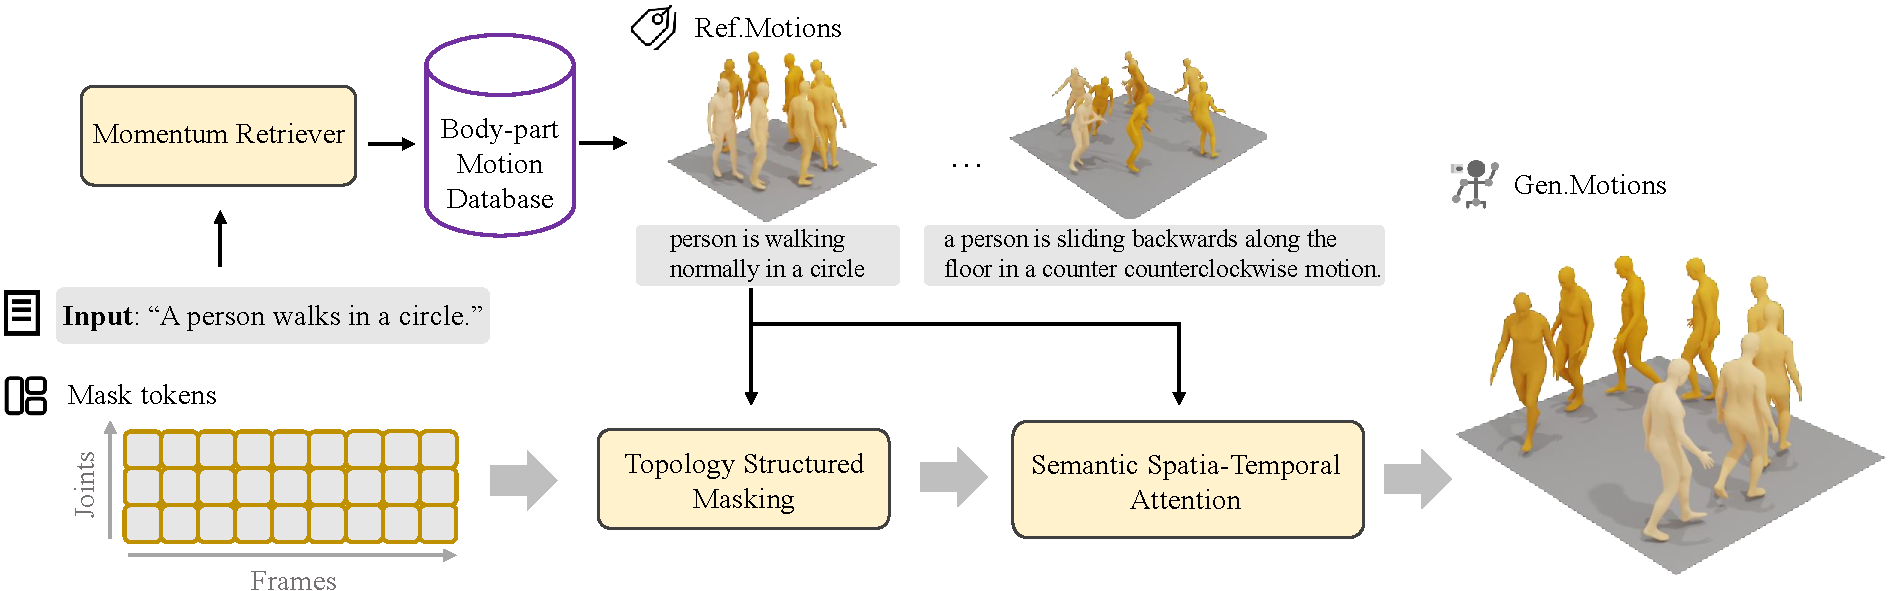
\includegraphics[width=\linewidth]{fig/teaser.pdf}
        \caption{\textbf{Overview of ReMoMask vs.\ ReMoMask-2.} ReMoMask retrieves in a contrastive semantic space and fuses evidence across a representation gap; ReMoMask-2 retrieves directly in the generator's pre-quantization latent space $z_e$ via a distilled query projector $\phi$, improving generation quality (\textbf{[TBD]}).}
        \label{fig:teaser}
\end{figure}

The second line of work, known as \emph{retrieval-augmented T2M (RAG-T2M)}, enhances generation by retrieving relevant motion–text pairs from an external database and injecting the retrieved evidence into the generative process. By conditioning generation on exemplar motions, RAG-based approaches improve robustness to uncommon or complex textual inputs. Representative methods include ReMoDiffuse~\cite{remodiffuse}, which performs retrieval via text–text similarity using CLIP~\cite{clip}, and ReMoGPT~\cite{remogpt}, which adopts a cross-modal text–motion retriever.

\begin{table}[t]
\centering
\caption{Comparison of different architecture designs.}
% \setlength{\tabcolsep}{4pt}
% \small % Adjust the font size
\setlength{\tabcolsep}{8pt}
\resizebox{\columnwidth}{!}{
    \begin{tabular}{l | c | c | c | c | c | c }
        \toprule
        % Method & Global Align & Part Align & Momentum & Gen.-Aligned & Fusion & Latent \\

        \multirow{2}{*}{Method} & \multicolumn{4}{c|}{Retrieval} & \multicolumn{2}{c}{Generation} \\
        \cline{2-7}

        & Global Align & Part Align & Momentum & Gen.-Aligned & Fusion & Latent \\

        \hline
        \hline

        MDM~\cite{mdm} &  -  & - & - & - & concat & 1D  \\

        T2M-GPT~\cite{t2m-gpt} &  -  & - & - & - & concat & 1D  \\

        MoMask~\cite{momask} &  -  & - & - & - & concat & 1D  \\

        MARDM~\cite{mardm} &  -   & -  & - & - & concat & 1D  \\

        LaMP~\cite{lamp} & -  & - & - & - & cross-attn & 1D  \\

        TMR~\cite{tmr} & $\checkmark$  & $\times$  & $\times$ & $\times$ & concat & 1D  \\

        MoRAG~\cite{morag} &  $\times$   & $\times$  & $\times$ & $\times$ & cross-attn & 1D  \\

        ReMoGPT~\cite{remogpt} & $\checkmark$  & $\times$  & $\times$ & $\times$ & concat & 1D  \\

        ReMoDiffuse~\cite{remodiffuse} & $\checkmark$  & $\times$  & $\times$ & $\times$ & cross-attn & 1D  \\

        % MoGenTS~\cite{mogents} &  $\times$   & $\times$  & $\times$ & concat & 2D  \\
        \midrule
        ReMoMask &  $\checkmark$   & $\checkmark$  & $\checkmark$ & $\times$ & SSTA & 2D  \\
        \rowcolor{yellow!20}\textbf{ReMoMask-2} &  $\checkmark$   & $\checkmark$  & $\checkmark$ & $\checkmark$ & SSTA & 2D  \\
        \bottomrule
    \end{tabular}
}

\label{tab:delta}
\end{table}

Despite their promising performance, existing RAG-T2M methods implicitly treat retrieval and fusion as independent modules and largely ignore the \emph{structural consistency} between retrieval alignment and motion representation. Through careful analysis, we identify two fundamental design axes in retrieval-augmented motion generation:


% \begin{table*}[t]
% \centering
% \caption{Comparison of different architecture designs.}
% \setlength{\tabcolsep}{4pt}
% \small % Adjust the font size
% \setlength{\tabcolsep}{8pt}
% \resizebox{\columnwidth}{!}{
%     \begin{tabular}{l | c | c | c | c | c }
%         \toprule
        % Method & Global Align & Part Align & Momentum & Fusion & Latent \\

%         \multirow{2}{*}{Method} & \multicolumn{3}{c|}{Retrieval} & \multicolumn{2}{c}{Generation} \\
%         \cline{2-6}
        
%         & Global Align & Part Align & Momentum & Fusion & Latent \\
        
%         \hline
%         \hline

%         MDM~\cite{mdm} &  -  & - & - & concat & 1D  \\

%         T2M-GPT~\cite{t2m-gpt} &  -  & - & - & concat & 1D  \\

%         MoMask~\cite{momask} &  -  & - & - & concat & 1D  \\

%         MARDM~\cite{mardm} &  -   & -  & - & concat & 1D  \\

%         LaMP~\cite{lamp} & -  & - & - & cross-attn & 1D  \\

%         TMR~\cite{tmr} & $\checkmark$  & $\times$  & $\times$ & concat & 1D  \\

%         MoRAG~\cite{morag} &  $\times$   & $\times$  & $\times$ & cross-attn & 1D  \\

%         ReMoGPT~\cite{remogpt} & $\checkmark$  & $\times$  & $\times$ & concat & 1D  \\

%         ReMoDiffuse~\cite{remodiffuse} & $\checkmark$  & $\times$  & $\times$ & cross-attn & 1D  \\


        
        % MoGenTS~\cite{mogents} &  $\times$   & $\times$  & $\times$ & concat & 2D  \\

%         Ours &  $\checkmark$   & $\checkmark$  & $\checkmark$ & SSTA & 2D  \\
%         \bottomrule
%     \end{tabular}
% }

% % \label{tab:delta}
% \end{table*}


\textbf{(1) Structural granularity of alignment.}  
As shown in Table~\ref{tab:delta}, most text–motion retrieval methods rely on contrastive learning to align global motion embeddings with text~\cite{tmr,temos}. However, human motion is inherently hierarchical, organized by skeletal topology and body-part dependencies. Purely global alignment overlooks fine-grained part-level semantics (e.g., left/right limbs or asymmetric actions), limiting retrieval discriminability. Although some works~\cite{remogpt,parco} encode part-level motion features, these representations are typically aggregated without part-level cross-modal alignment, weakening structured correspondence.

\textbf{(2) Structural compatibility of fusion.}  
% Beyond retrieval, retrieved evidence must be injected into the generative backbone in a way that respects motion topology. 
As depicted in Table~\ref{tab:delta}, existing RAG-T2M methods often adopt simple concatenation or vanilla cross-attention, without systematically examining how motion latent structure (e.g., 1D vs. 2D spatial–temporal tokens) interacts with fusion mechanisms. This mismatch between retrieved information and motion representation can limit generation quality.


These observations suggest that performance improvements in RAG-T2M are not merely determined by stronger individual modules, but by whether \emph{retrieval alignment and fusion design are structurally consistent with motion topology}.

In this work, we propose \textbf{ReMoMask}, a retrieval-augmented masked generative framework for text-to-motion generation. 
To address alignment granularity, we introduce \textbf{H}ierarchical \textbf{B}idirectional \textbf{M}omentum (HBM) alignment, a structured contrastive learning framework that jointly supervises instance-level (global) and part-level bidirectional text–motion correspondence under a momentum-based paradigm. 

To ensure structural compatibility during semantic conditioning, we conduct a systematic study (provided in Section~\ref{sec:preliminary}) on motion latent representations and fusion strategies. 
Our analysis reveals that preserving motion as 2D spatial–temporal tokens, rather than flattening them into 1D sequences, significantly improves semantic injection and generation stability. 
Motivated by this observation, we design \textbf{S}emantic \textbf{S}patial-\textbf{T}emporal \textbf{A}ttention (SSTA), an attention mechanism tailored to inject retrieved motion semantics into the generative backbone. Meanwhile, to further strengthen structural modeling within this 2D formulation, we adopt a \textbf{T}opology \textbf{S}tructured \textbf{M}asking (TSM) strategy, allowing the network to learn richer topological dependencies across body parts and time.

Beyond these two axes, a third design dimension has so far remained implicit: \textbf{(3) Representation consistency of the retrieval space.} Existing RAG-T2M systems retrieve in an embedding space that is decoupled from the space in which generation actually takes place. ReMoDiffuse~\cite{remodiffuse} retrieves via text--text similarity in the CLIP space~\cite{clip}, while cross-modal retrievers such as ReMoGPT~\cite{remogpt}---and the HBM retriever of our conference version---operate in a contrastively learned text--motion semantic space. The generator, in contrast, manipulates the latents of its own residual vector-quantized VAE (RVQ-VAE). Retrieved evidence must therefore cross a \emph{representation gap} before it can condition generation: exemplars that are close in the retrieval space need not be close in the space the generator synthesizes in, and the fusion module has to translate between the two representations implicitly.

In this article, we extend our conference framework along this third axis and present \textbf{ReMoMask-2} (Fig.~\ref{fig:teaser}). Instead of retrieving in a separate semantic space, ReMoMask-2 builds its retrieval database directly in the generator's pre-quantization latent space $z_e$: motions are encoded by the frozen RVQ-VAE encoder, and text queries are mapped into the same space by a lightweight query projector $\phi$ ($\sim$1.57M parameters) trained by knowledge distillation from the HBM retriever. Retrieved evidence and the generative substrate thus share a single representation, and the SSTA fusion module is reused unchanged up to two linear adapters. Latent alignment also changes the premise of a design decision made in the conference version: once the retrieved text embedding $R_t$ is projected into the motion-aligned space, it is no longer a cross-domain signal, which re-opens the question of whether it should enter the Value pathway of SSTA (Section~\ref{subsec:vroute}).

Our contributions are summarized as follows:

\begin{itemize}
    \item We identify two key structural design axes—alignment granularity and fusion compatibility—in text-to-motion generation, and demonstrate that enforcing structural consistency across alignment, representation, and fusion is critical for high-quality motion synthesis.
    
    \item We propose \textbf{HBM}, a hierarchical bidirectional momentum alignment framework that explicitly models both global and part-level text–motion correspondence, enhancing fine-grained semantic grounding.
    
    \item We design \textbf{SSTA}, a topology-aware spatial–temporal attention mechanism built upon structured 2D motion tokens, together with a \textbf{TSM} masking strategy that strengthens topological dependencies across body parts and time.
    
    \item Extensive experiments on HumanML3D, KIT-ML, and SnapMoGen show that ReMoMask achieves state-of-the-art performance in both motion generation and cross-modal retrieval, validating the effectiveness of structure-aware masked modeling.

    \item We identify a third structural design axis in retrieval-augmented motion generation---\emph{representation consistency between the retrieval space and the generative latent space}---and show that in existing RAG-T2M systems, including our conference version, retrieved evidence lives in a space decoupled from the latents the generator manipulates.

    \item We present \textbf{ReMoMask-2}, a latent-aligned retrieval framework that builds the retrieval database in the pre-quantization latent space $z_e$ of the frozen RVQ-VAE and maps text queries into the same space with a lightweight projector $\phi$ distilled from the HBM retriever via KL-based soft-ranking supervision. The generative backbone and SSTA are architecturally untouched save for two linear adapters, and generation quality improves consistently over ReMoMask (\textbf{[TBD]} FID reduction on HumanML3D).

    \item As an orthogonal minor contribution, we revisit the value-pathway routing of SSTA: once $R_t$ is projected into the motion-aligned latent space, the domain-mismatch premise for excluding textual evidence from the Value pathway no longer applies, and re-admitting $R_t$ is beneficial (\textbf{[TBD]}).
\end{itemize}

A preliminary version of this work, ReMoMask, was presented at ECCV 2025~\cite{remomask}.
This paper extends our conference version in the following aspects. (i)~We introduce a latent-aligned retrieval framework (Section~\ref{subsec:lar}) that relocates the retrieval database to the pre-quantization latent space $z_e$ of the generator's frozen RVQ-VAE, with text queries aligned to it by projector distillation, so that retrieval and generation operate on one representation. (ii)~We revisit the value-pathway routing of SSTA (Section~\ref{subsec:vroute}): latent alignment turns the retrieved text embedding $R_t$ into a motion-domain signal, changing the premise under which the conference version excluded textual evidence from the Value pathway. (iii)~We provide a geometric analysis of the $z_e$ space (Section~\ref{sec:preliminary}) that establishes the feasibility of latent-space retrieval and grounds the third design axis. (iv)~We add new orthogonal ablations (retrieval space $\times$ value routing, alignment objective, and teacher choice; Section~\ref{subsec:ablation_v2}) and a full-pipeline evaluation of ReMoMask-2 against ReMoMask under an identical training configuration, while retaining all conference results.

% \begin{figure*}[t!]
%     \centering
%     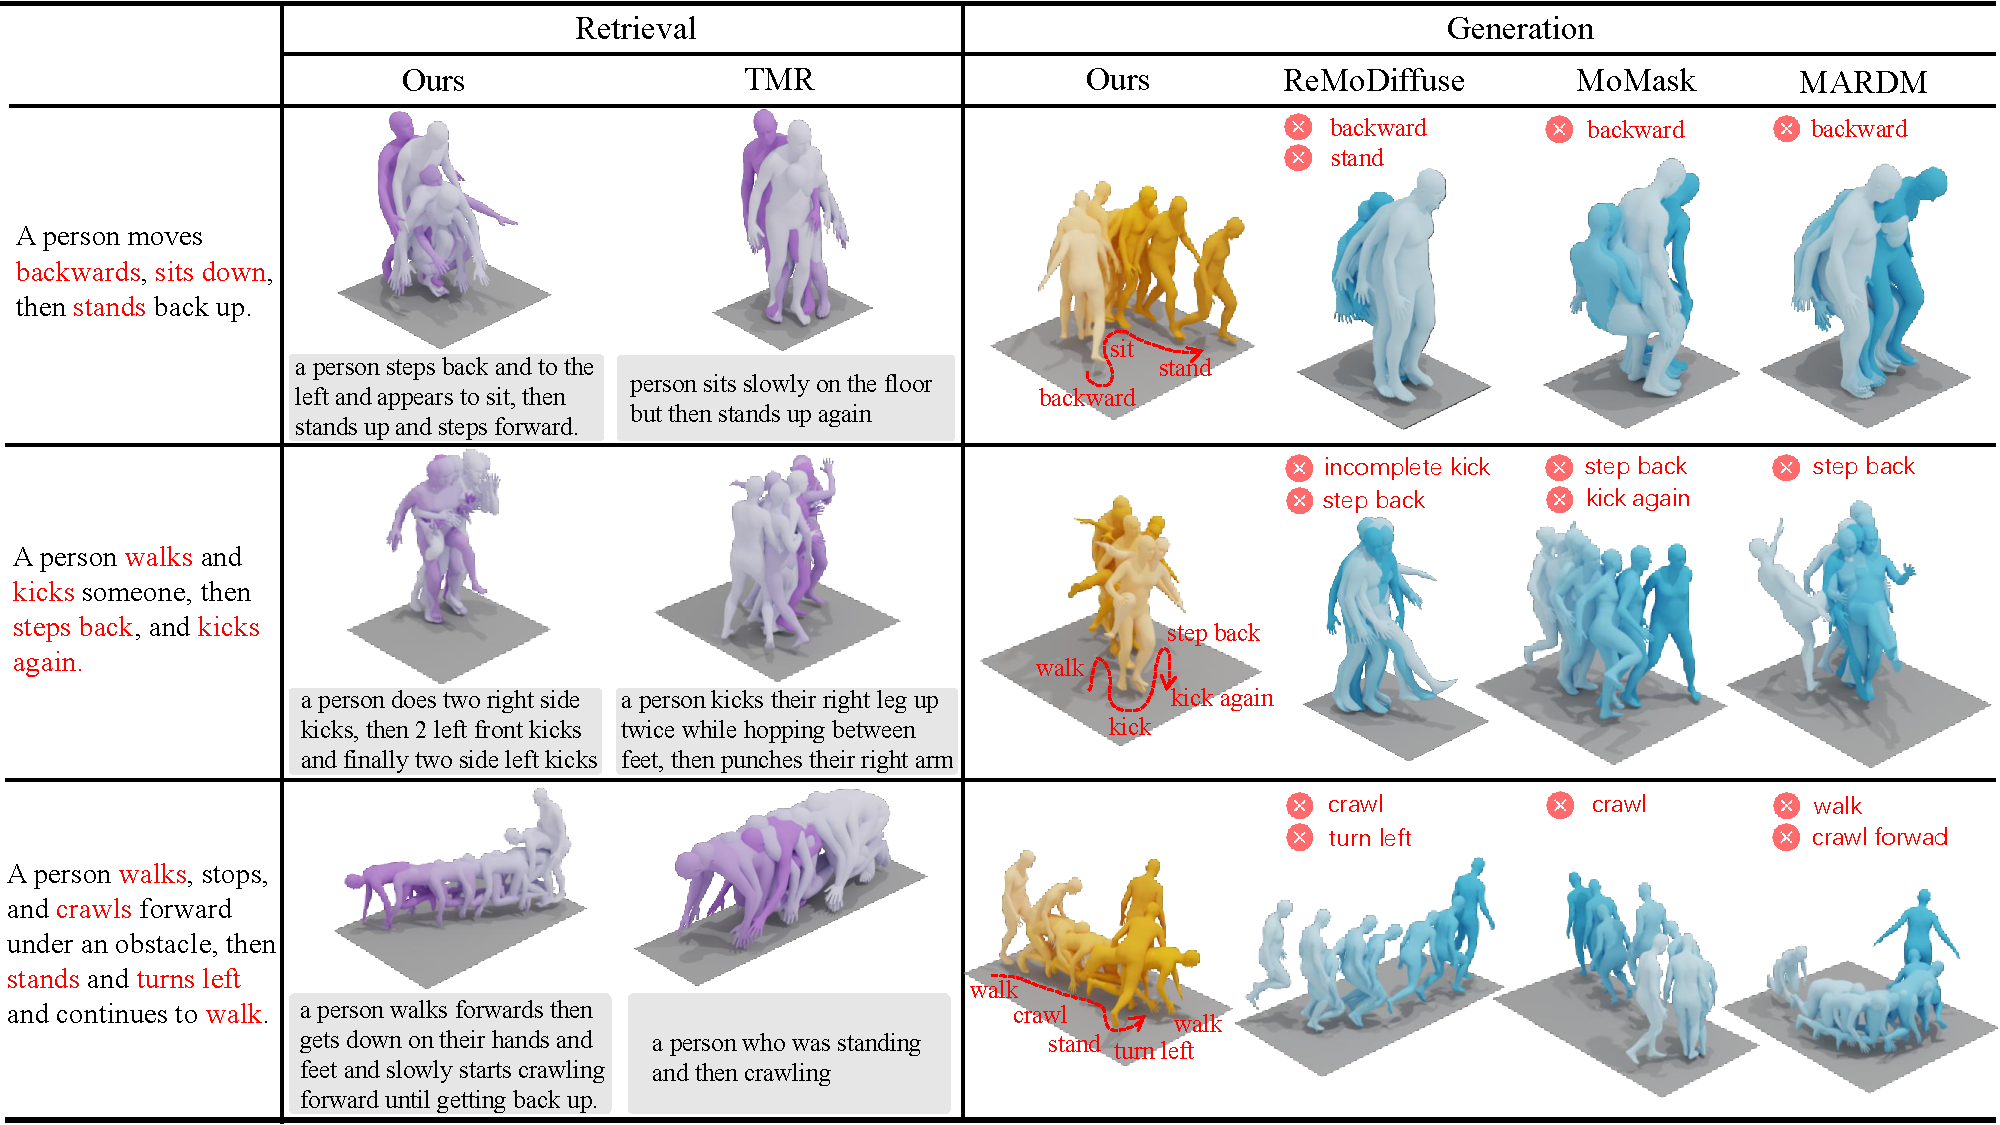
\includegraphics[width=\linewidth]{fig/rag_t2m_visual.pdf}
%         % \caption{\textbf{Heatmap of similarity matrix.} The diagonal represents positive pairs, with darker colors meaning higher semantic similarity, conducted on HumanML3D.}
%      \caption{\textbf{Qualitative comparisons.} The darker colors indicate the later in time. The motions generated by our method closely align with the descriptions, outperforming others that exhibit degraded motions or improper semantics.}
%     %     \label{fig:rag_t2m_visual}
% \end{figure*}


\begin{figure*}[t!]
    \centering
    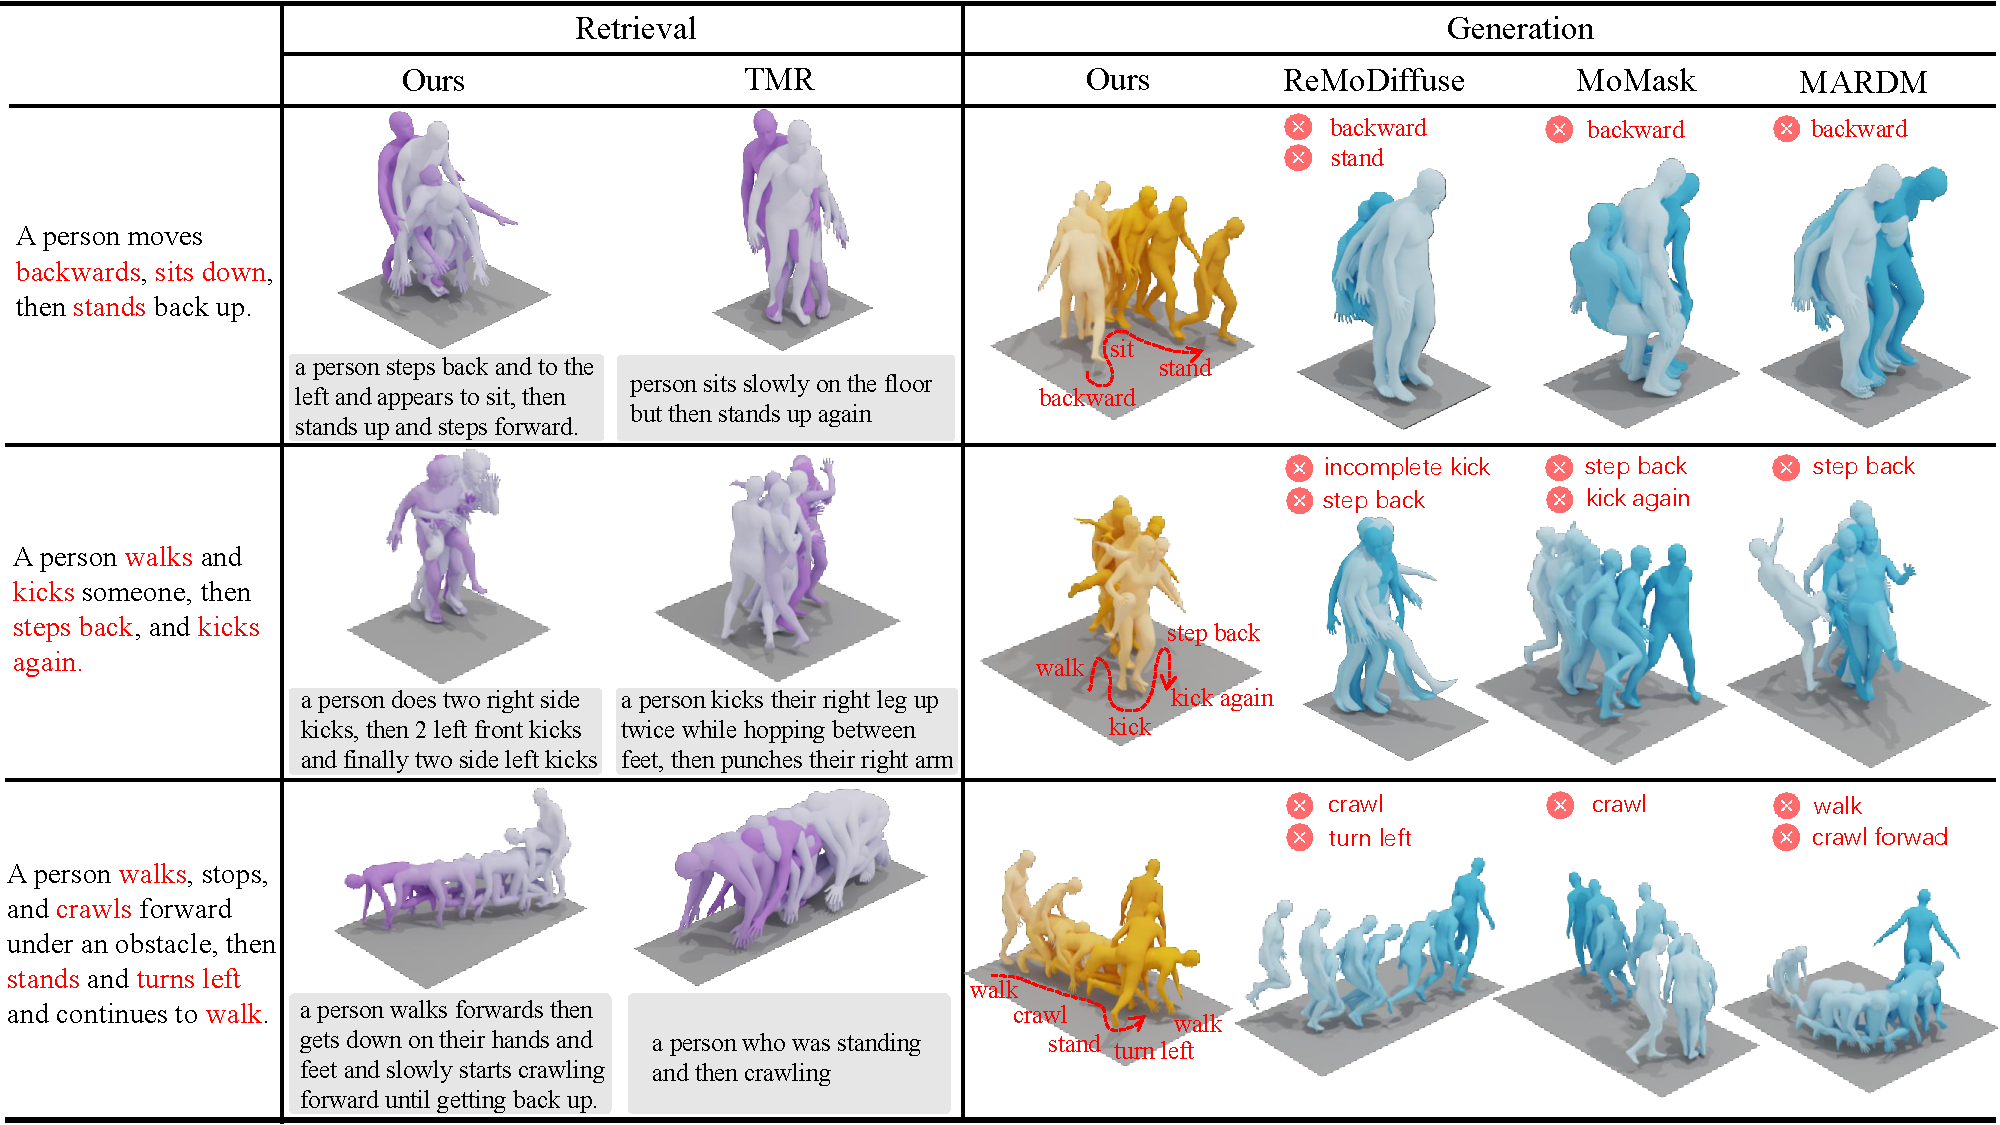
\includegraphics[width=\linewidth]{fig/rag_t2m_visual.pdf}
        % \caption{\textbf{Heatmap of similarity matrix.} The diagonal represents positive pairs, with darker colors meaning higher semantic similarity, conducted on HumanML3D.}
     \caption{\textbf{Qualitative comparisons.} The darker colors indicate the later in time. The motions generated by our method closely align with the descriptions, outperforming others that exhibit degraded motions or improper semantics.}
        \label{fig:rag_t2m_visual}
\end{figure*}
% \begin{table*}[t]
% \centering
% \caption{Comparison of different architecture designs.}
% \setlength{\tabcolsep}{4pt}
% \small % Adjust the font size
% \setlength{\tabcolsep}{8pt}
% \resizebox{\columnwidth}{!}{
%     \begin{tabular}{l | c | c | c | c | c }
%         \toprule
        % Method & Global Align & Part Align & Momentum & Fusion & Latent \\

%         \multirow{2}{*}{Method} & \multicolumn{3}{c|}{Retrieval} & \multicolumn{2}{c}{Generation} \\
%         \cline{2-6}
        
%         & Global Align & Part Align & Momentum & Fusion & Latent \\
        
%         \hline
%         \hline

%         MDM~\cite{mdm} &  -  & - & - & concat & 1D  \\

%         T2M-GPT~\cite{t2m-gpt} &  -  & - & - & concat & 1D  \\

%         MoMask~\cite{momask} &  -  & - & - & concat & 1D  \\

%         MARDM~\cite{mardm} &  -   & -  & - & concat & 1D  \\

%         LaMP~\cite{lamp} & -  & - & - & cross-attn & 1D  \\

%         TMR~\cite{tmr} & $\checkmark$  & $\times$  & $\times$ & concat & 1D  \\

%         MoRAG~\cite{morag} &  $\times$   & $\times$  & $\times$ & cross-attn & 1D  \\

%         ReMoGPT~\cite{remogpt} & $\checkmark$  & $\times$  & $\times$ & concat & 1D  \\

%         ReMoDiffuse~\cite{remodiffuse} & $\checkmark$  & $\times$  & $\times$ & cross-attn & 1D  \\


        
        % MoGenTS~\cite{mogents} &  $\times$   & $\times$  & $\times$ & concat & 2D  \\

%         Ours &  $\checkmark$   & $\checkmark$  & $\checkmark$ & SSTA & 2D  \\
%         \bottomrule
%     \end{tabular}
% }

% % \label{tab:delta}
% \end{table*}

\section{Related Work}
\label{sec:relatedwork}
% \begin{figure*}[t!]
%     \centering
%     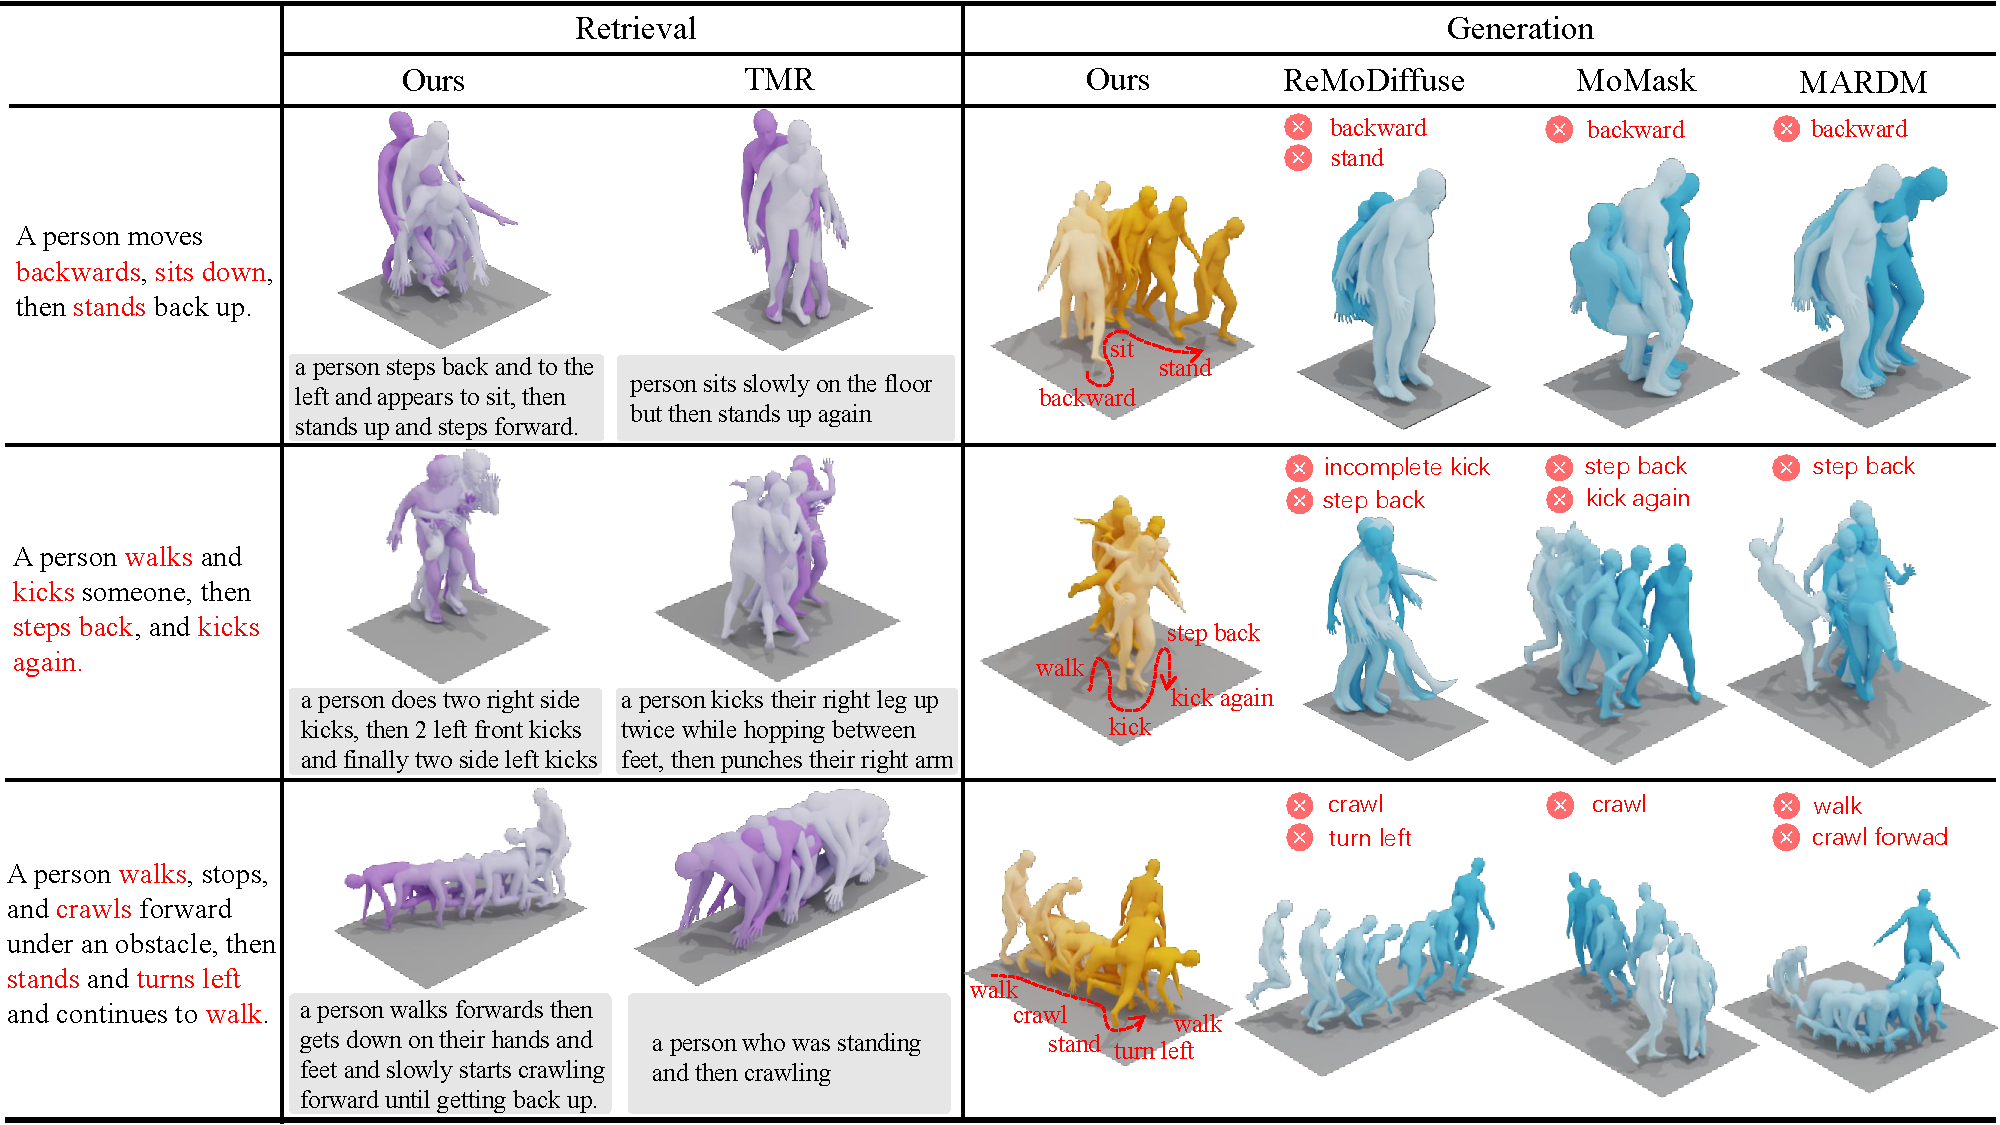
\includegraphics[width=\linewidth]{fig/rag_t2m_visual.pdf}
%         % \caption{\textbf{Heatmap of similarity matrix.} The diagonal represents positive pairs, with darker colors meaning higher semantic similarity, conducted on HumanML3D.}
%      \caption{\textbf{Qualitative comparisons.} The darker colors indicate the later in time. The motions generated by our method closely align with the descriptions, outperforming others that exhibit degraded motions or improper semantics.}
%     %     \label{fig:rag_t2m_visual}
% \end{figure*}

\subsection{Text-to-Motion Generation}

Text-to-motion (T2M) generation aims to synthesize realistic human motion sequences conditioned on natural language descriptions. Early approaches explored adversarial learning to establish text–motion correspondence. With the introduction of vector quantization, TM2T~\cite{tm2t} and T2M-GPT~\cite{t2m-gpt} discretized motion sequences and leveraged autoregressive transformers for semantic control. However, autoregressive decoding often suffers from error accumulation.

Recent advances focus on improving motion representation and generation paradigms. MoMask~\cite{momask} introduces hierarchical residual quantization and masked bidirectional transformers for parallel decoding, achieving strong performance on HumanML3D. Diffusion-based methods~\cite{ddpms,motiongpt} further enhance generation quality via non-autoregressive denoising processes. MotionGPT~\cite{motiongpt} unifies multiple generation tasks under a discrete autoregressive framework. 

Beyond backbone improvements, several works investigate fine-grained motion structure modeling. ParCo~\cite{parco} discretizes whole-body motion into part-level components (limbs, backbone, root) to establish structured priors.

% These methods demonstrate that explicitly modeling motion topology can improve controllability and representation quality.

% However, most prior T2M methods focus on strengthening the generative backbone, while retrieval-based enhancements introduce additional structural considerations regarding cross-modal alignment and information fusion.






\subsection{Retrieval-Augmented Text-to-Motion}

Retrieval-augmented generation (RAG) has been extended beyond NLP to multimodal domains, including motion generation~\cite{rmd,remodiffuse,morag,remogpt}. In retrieval-augmented T2M (RAG-T2M), relevant motion–text pairs are retrieved from an external database and injected into the generative backbone to improve robustness under complex or rare textual conditions. 

Existing approaches typically rely on global contrastive alignment between text and motion embeddings~\cite{tmr,temos}. For instance, ReMoDiffuse~\cite{remodiffuse} performs retrieval based on text–text similarity to indirectly guide generation, while ReMoGPT~\cite{remogpt} introduces part-aware encoders for cross-modal retrieval. However, these methods often aggregate part features without explicit bidirectional cross-modal supervision, leaving fine-grained structural correspondence between text descriptions and specific body parts underexplored. Furthermore, regarding the integration of retrieved information, prior works commonly adopt feature concatenation or standard cross-attention~\cite{remodiffuse,remogpt} without systematically considering the compatibility between the retrieved evidence and the underlying motion latent topology. The impact of motion representation structures on fusion effectiveness remains largely uninvestigated.

A trait common to these systems---and to the conference version of this work---is that the retrieval space is decoupled from the generative representation: queries and keys live in the CLIP text space~\cite{clip,remodiffuse} or in a contrastively learned text--motion embedding space~\cite{tmr,remogpt}, whereas the generator operates on the latents of its own RVQ-VAE, so retrieved exemplars must be translated across representations at fusion time. In other modalities, retrieving directly in the generative model's own representation space has proven effective; for example, AR-RAG~\cite{qi2025ar} retrieves patch-level visual tokens during autoregressive image generation, and language models have been augmented with neighbors retrieved in their own embedding spaces.
% TODO-CITE: kNN-LM (Khandelwal et al., ICLR 2020) and RETRO (Borgeaud et al.,
% ICML 2022) — retrieval keyed on the language model's own representations.
% TODO-CITE: retrieval-augmented diffusion models (Blattmann et al., NeurIPS
% 2022) — nearest-neighbour conditioning for image synthesis in a learned
% feature space.
In Section~\ref{subsec:lar} we transfer this principle to motion generation: ReMoMask-2 keys its database on the generator's own pre-quantization latents, so no representation gap separates retrieval from generation.

% In contrast, our work explicitly addresses these limitations by investigating the structural consistency between retrieval alignment and motion representation. We jointly enforce hierarchical bidirectional alignment to capture fine-grained semantics and design a topology-aware fusion module tailored for 2D spatial–temporal motion tokens, effectively bridging the gap between structured retrieval and structured generation.







% \subsection{Retrieval-Augmented Text-to-Motion}

% Retrieval-augmented generation (RAG) has been extended beyond NLP to multimodal domains, including motion generation~\cite{remodiffuse,morag,remogpt}. In retrieval-augmented T2M (RAG-T2M), relevant motion–text pairs are retrieved from an external database and injected into the generative backbone to improve robustness under complex or rare textual conditions. Existing RAG-T2M methods primarily differ along two dimensions: alignment granularity and fusion mechanism.

% \textbf{Alignment Granularity.}  
% Most text–motion retrieval models rely on global contrastive alignment between text and motion embeddings~\cite{tmr,temos}. ReMoDiffuse~\cite{remodiffuse} performs retrieval based on text–text similarity, indirectly guiding motion generation. ReMoGPT~\cite{remogpt} introduces cross-modal retrieval with part-aware motion encoders; however, part features are typically aggregated without explicit bidirectional cross-modal supervision. As a result, fine-grained structural correspondence between text and body parts remains underexplored.

% \textbf{Fusion Mechanism.}  
% After retrieval, injected information must be integrated into the generative model. Prior works commonly adopt feature concatenation or vanilla cross-attention~\cite{remodiffuse,remogpt}, without explicitly considering the compatibility between retrieved evidence and motion latent topology. In particular, the interaction between motion representation and fusion design has not been systematically studied. 

% In contrast to these approaches, our work explicitly investigates the structural consistency between retrieval alignment and motion representation. We jointly enforce hierarchical bidirectional alignment and design a topology-aware fusion module tailored for 2D spatial–temporal motion tokens, bridging the gap between structured retrieval and structured generation.




% \section{Design Principles of Retrieval-Augmented Motion Generation}
% \label{sec:preliminary}
\begin{table}[t]
% \begin{table}[t]
    \centering
    \caption{Comparison of different latent structures and fusion strategies.}
    \label{tab:prelimi_experiment}
    \renewcommand{\arraystretch}{1.5}  % Adjust the line height (global)
    \setlength{\tabcolsep}{4pt}  % Adjust the column margin
    \resizebox{\columnwidth}{!}{
        \begin{tabular}{l| c| c| c| c }
            \toprule
            Generator & Latent & Fusion & FID$\downarrow$ & Top1$\uparrow$ \\
            \hline
            \hline
            
            \multirow{4}{*}{MoMask} & \multirow{2}{*}{1D} & concat    & $0.057^{\pm.013}$ & $0.511^{\pm{.003}}$ \\
            &  & crossAttn & $\underline{0.0 43^{\pm{.004}}}$ & $\underline{0.525^{\pm{.003}}}$  \\
            \cline{2-5}
             & \multirow{2}{*}{2D} & concat    & $0.049^{\pm{.007}}$ & $0.518^{\pm{.003}}$   \\
            & & crossAttn & $\mathbf{0.036^{\pm .005}}$ & $\mathbf{0.536^{\pm{.002}}}$  \\
            \bottomrule
        \end{tabular}
    }
% \end{table}
\end{table}

% Although retrieval-augmented T2M methods have shown promising improvements, the interaction between motion representation and fusion strategy remains insufficiently understood. Rather than treating retrieval and fusion as independent components, we aim to identify the structural design principles that govern effective retrieval injection in motion generation.
% We focus on two key design axes: (1) \emph{motion latent topology}, i.e., whether motion is represented as a 1D token sequence or a 2D spatial–temporal token grid (joint $\times$ time), and (2) \emph{fusion mechanism}, i.e., how retrieved information is integrated into the generative backbone, via feature concatenation or attention-based interaction.

% To isolate the effect of these axes, we conduct controlled experiments by systematically varying motion representation and fusion strategy while keeping all other components fixed. 
% Specifically, we adopt MoMask~\cite{momask} as a unified generative backbone and modify its motion latent formulation to construct both 1D token sequences $z_{1d}$ and 2D spatial–temporal token grids $z_{2d}$. 

% % This controlled setup ensures that the generative architecture, training procedure, and optimization settings remain identical, allowing us to focus solely on the structural impact of latent topology and fusion mechanism.
% For semantic retrieval, we employ a pretrained retriever from ReMoDiffuse~\cite{remodiffuse} checkpoint trained on the HumanML3D training split to obtain motion embeddings $R_m$ and text embeddings $R_t$, with the prompt embedding denoted as $t$. 
% Retrieved representations are then integrated into the generator via either feature concatenation or attention-based interaction, enabling fair comparison between fusion strategies under consistent backbone settings.

% Table~\ref{tab:prelimi_experiment} summarizes the results. 
% We observe consistent improvements when moving from 1D to 2D motion latents and when replacing concatenation with attention-based fusion. 
% Notably, the combination of 2D spatial–temporal representation and cross-attention achieves the best overall performance, suggesting that motion topology and fusion design interact in a complementary manner rather than contributing independently.


% These observations suggest a fundamental design principle for retrieval augmented T2M: \emph{retrieved evidence must be injected in a manner that preserves and interacts with the spatial–temporal topology of motion representations}. This structural compatibility explains the limitations of naive concatenation under 1D latents and directly motivates our fusion module, SSTA, which is particularly suited to fuse motion tokens and retrieved semantics.



%%%%%%%%%%%%%%%%%%%%%%%%%%%%%%%% V2 %%%%%%%%%%%%%%%%%%%%%%%%%%%%%%%%%%
% \section{Design Principles of Retrieval-Augmented Motion Generation}
% \label{sec:preliminary}
% \begin{table}[t]
% \begin{table}[t]
% %     \centering
%     \caption{Comparison of different latent structures and fusion strategies.}
%     \label{tab:prelimi_experiment}
%     \renewcommand{\arraystretch}{1.5}  % Adjust the line height (global)
%     \setlength{\tabcolsep}{4pt}  % Adjust the column margin
%     \resizebox{0.5\columnwidth}{!}{
%         \begin{tabular}{l| c| c| c| c }
%             \toprule
%             Generator & Latent & Fusion & FID$\downarrow$ & Top1$\uparrow$ \\
%             \hline
%             \hline
            
%             \multirow{4}{*}{MoMask} & \multirow{2}{*}{1D} & concat    & $0.057^{\pm.013}$ & $0.511^{\pm{.003}}$ \\
%             &  & crossAttn & $\underline{0.0 43^{\pm{.004}}}$ & $\underline{0.525^{\pm{.003}}}$  \\
%             \cline{2-5}
%              & \multirow{2}{*}{2D} & concat    & $0.049^{\pm{.007}}$ & $0.518^{\pm{.003}}$   \\
%             & & crossAttn & $\mathbf{0.036^{\pm .005}}$ & $\mathbf{0.536^{\pm{.002}}}$  \\
%             \bottomrule
%         \end{tabular}
%     }
% \end{table}
% % \end{table}


% While retrieval-augmented T2M methods show promise, the interplay between motion representation and fusion strategy remains underexplored. We investigate two key design axes: (1) \emph{motion latent topology} (1D token sequence vs. 2D spatial–temporal grid) and (2) \emph{fusion mechanism} (feature concatenation vs. attention-based interaction).

% Using MoMask~\cite{momask} as a unified backbone, we systematically vary these axes while fixing all other components. We construct both 1D ($z_{1d}$) and 2D ($z_{2d}$) latents, integrating retrieved embeddings ($R_m, R_t$ from ReMoDiffuse~\cite{remodiffuse}) via concatenation or cross-attention. 

% As summarized in Table~\ref{tab:prelimi_experiment}, shifting from 1D to 2D latents and from concatenation to attention yields consistent improvements. The optimal configuration combines 2D spatial–temporal representation with cross-attention, indicating that motion topology and fusion design are complementary. This suggests a core principle: \emph{retrieved evidence must preserve and interact with the spatial–temporal topology of motion}. This insight directly motivates our SSTA module, designed to effectively fuse motion tokens with retrieved semantics.



%%%%%%%%%%%%%%%%%%%%%%%%%%%%%%%% V3 %%%%%%%%%%%%%%%%%%%%%%%%%%%%%%%%%%
\section{Design Principles of Retrieval-Augmented Motion Generation}
\label{sec:preliminary}
% \begin{table}[t]
% \begin{table}[t]
% %     \centering
%     \caption{Comparison of different latent structures and fusion strategies.}
%     \label{tab:prelimi_experiment}
%     \renewcommand{\arraystretch}{1.5}  % Adjust the line height (global)
%     \setlength{\tabcolsep}{4pt}  % Adjust the column margin
%     \resizebox{0.5\columnwidth}{!}{
%         \begin{tabular}{l| c| c| c| c }
%             \toprule
%             Generator & Latent & Fusion & FID$\downarrow$ & Top1$\uparrow$ \\
%             \hline
%             \hline
            
%             \multirow{4}{*}{MoMask} & \multirow{2}{*}{1D} & concat    & $0.057^{\pm.013}$ & $0.511^{\pm{.003}}$ \\
%             &  & crossAttn & $\underline{0.0 43^{\pm{.004}}}$ & $\underline{0.525^{\pm{.003}}}$  \\
%             \cline{2-5}
%              & \multirow{2}{*}{2D} & concat    & $0.049^{\pm{.007}}$ & $0.518^{\pm{.003}}$   \\
%             & & crossAttn & $\mathbf{0.036^{\pm .005}}$ & $\mathbf{0.536^{\pm{.002}}}$  \\
%             \bottomrule
%         \end{tabular}
%     }
% \end{table}
% % \end{table}


While retrieval-augmented T2M methods show promise, the interplay between motion representation and fusion strategy remains underexplored. We investigate two key design axes: (1) \emph{motion latent topology} (1D sequence vs. 2D spatial–temporal grid) and (2) \emph{fusion mechanism} (concatenation vs. cross-attention).

Using MoMask~\cite{momask} as a backbone generator, we systematically vary these axes while fixing other components. We construct both 1D ($z_{1d}$) and 2D ($z_{2d}$) latents, integrating retrieved embeddings ($R_m, R_t$ from ReMoDiffuse~\cite{remodiffuse}) via concatenation or cross-attention. All evaluations are performed on the HumanML3D benchmark.

As summarized in Table~\ref{tab:prelimi_experiment}, shifting to 2D latents and adopting cross-attention yields consistent improvements. The optimal configuration combines 2D representation with cross-attention, revealing that effective retrieval injection \emph{hinges on preserving the spatial–temporal topology while enabling structural interaction}. These dual findings directly motivate our \textbf{SSTA} module, which is explicitly designed to fuse retrieved semantics with motion tokens via structure-aware cross-attention over a 2D latent grid.

\noindent \myparagraph{Representation Consistency of the Retrieval Space.}
The preceding analysis concerns how the motion latent is structured and how retrieved evidence is fused; both questions presuppose that retrieval operates in a semantic space separate from the generator. A third question is whether the generator's \emph{own} latent space can serve as the retrieval space, so that retrieved evidence and the generative substrate share a single representation. To assess feasibility, we analyze the geometry of the pre-quantization latents $z_e$ produced by the frozen 2D-RVQ-VAE encoder~\cite{mogents}: each training motion is mean-pooled over its spatial--temporal grid and $\ell_2$-normalized, yielding one 1024-dimensional descriptor. Two findings emerge. First, the space does not collapse: pairwise cosine similarities average $0.62$ (std $0.25$, range $[-0.55, 0.998]$), leaving sufficient spread for discriminative cosine-based retrieval. Second, the space is strongly anisotropic: its effective dimensionality is only $11$ out of $1024$, and $7$ principal directions already explain $95\%$ of the variance. Latent-space retrieval is therefore feasible, but the geometry of $z_e$ differs markedly from that of contrastively learned semantic spaces, so text queries cannot be mapped into it heuristically. Indeed, directly comparing neighborhood structure across the two spaces (2,000 sampled training motions, cosine ranking) yields a mean Spearman correlation of only $0.58$ between their similarity rankings, and the top-$10$ nearest-neighbor sets overlap by merely $18\%$: the exemplars that semantic-space retrieval returns are, more than four times out of five, not the exemplars that are closest in the space the generator synthesizes in. These observations ground a third design axis---\emph{representation consistency between the retrieval space and the generative latent space}---which we instantiate with the latent-aligned retrieval framework of Section~\ref{subsec:lar}.

% Optional figure (enable once fig/ze_geometry.pdf is redrawn as vector art from
% cosine_sim_hist.png + eigenvalue_spectrum.png). When enabling, add
% "(Fig.~\ref{fig:ze_geometry})" after "Two findings emerge" in the paragraph
% above.
% \begin{figure}[t]
%     \centering
%     \includegraphics[width=\linewidth]{fig/ze_geometry.pdf}
%     \caption{\textbf{Geometry of the pre-quantization latent space $z_e$ on
%     HumanML3D.} Left: histogram of pairwise cosine similarities between pooled
%     motion latents (mean $0.62$, std $0.25$); the embeddings do not collapse.
%     Right: eigenvalue spectrum of the latent covariance; $7$ principal
%     directions explain $95\%$ of the variance and the effective dimensionality
%     is $11/1024$, indicating strong anisotropy.}
%     \label{fig:ze_geometry}
% \end{figure}






\section{Methodology}
\subsection{Overview}
\label{subsec:overview}
% \begin{figure*}[t] 
%     \centering
%     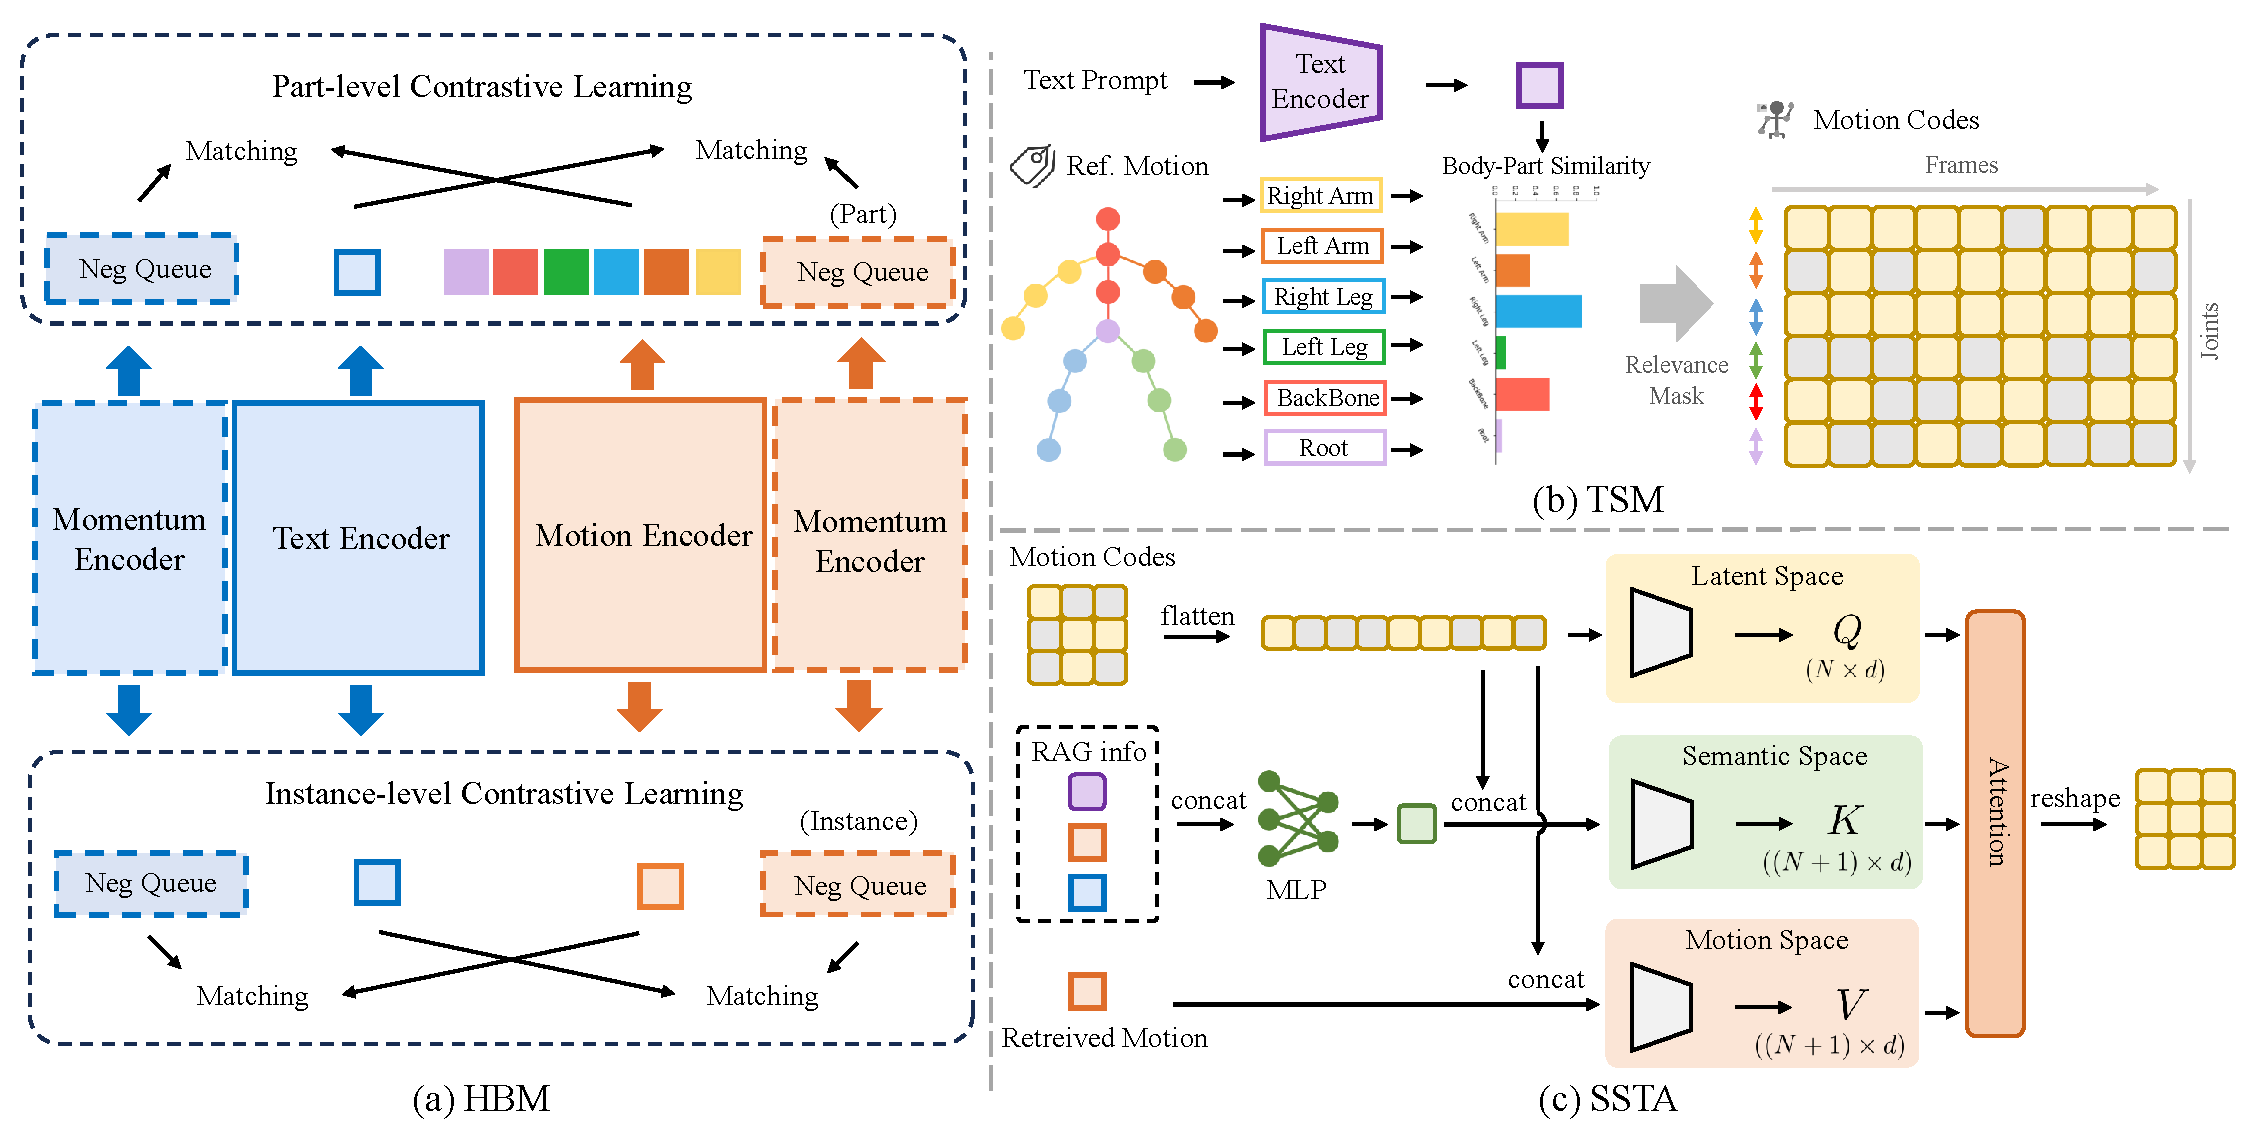
\includegraphics[width=\textwidth]{fig/framework.pdf} 
%     \caption{\textbf{Overview of ReMoMask}. (a) The overall retrieval-augmented text-to-motion pipeline, where retrieved text and motion embeddings are fused with latent motion tokens to guide motion generation. (b) \textbf{H}ierarchical \textbf{B}idirectional \textbf{M}omentum Contrastive Learning (HBM), which performs instance-level and part-level bidirectional alignment between text and motion using momentum encoders and negative queues. (c) \textbf{S}emantic \textbf{S}patial–\textbf{T}emporal \textbf{A}ttention (SSTA), which injects retrieved semantic information into spatial–temporal motion tokens by redefining the attention Q, K, V.
%     }
%     %     \label{fig:framework}
% \end{figure*}




% \begin{figure*}[t] 
%     \centering 
%     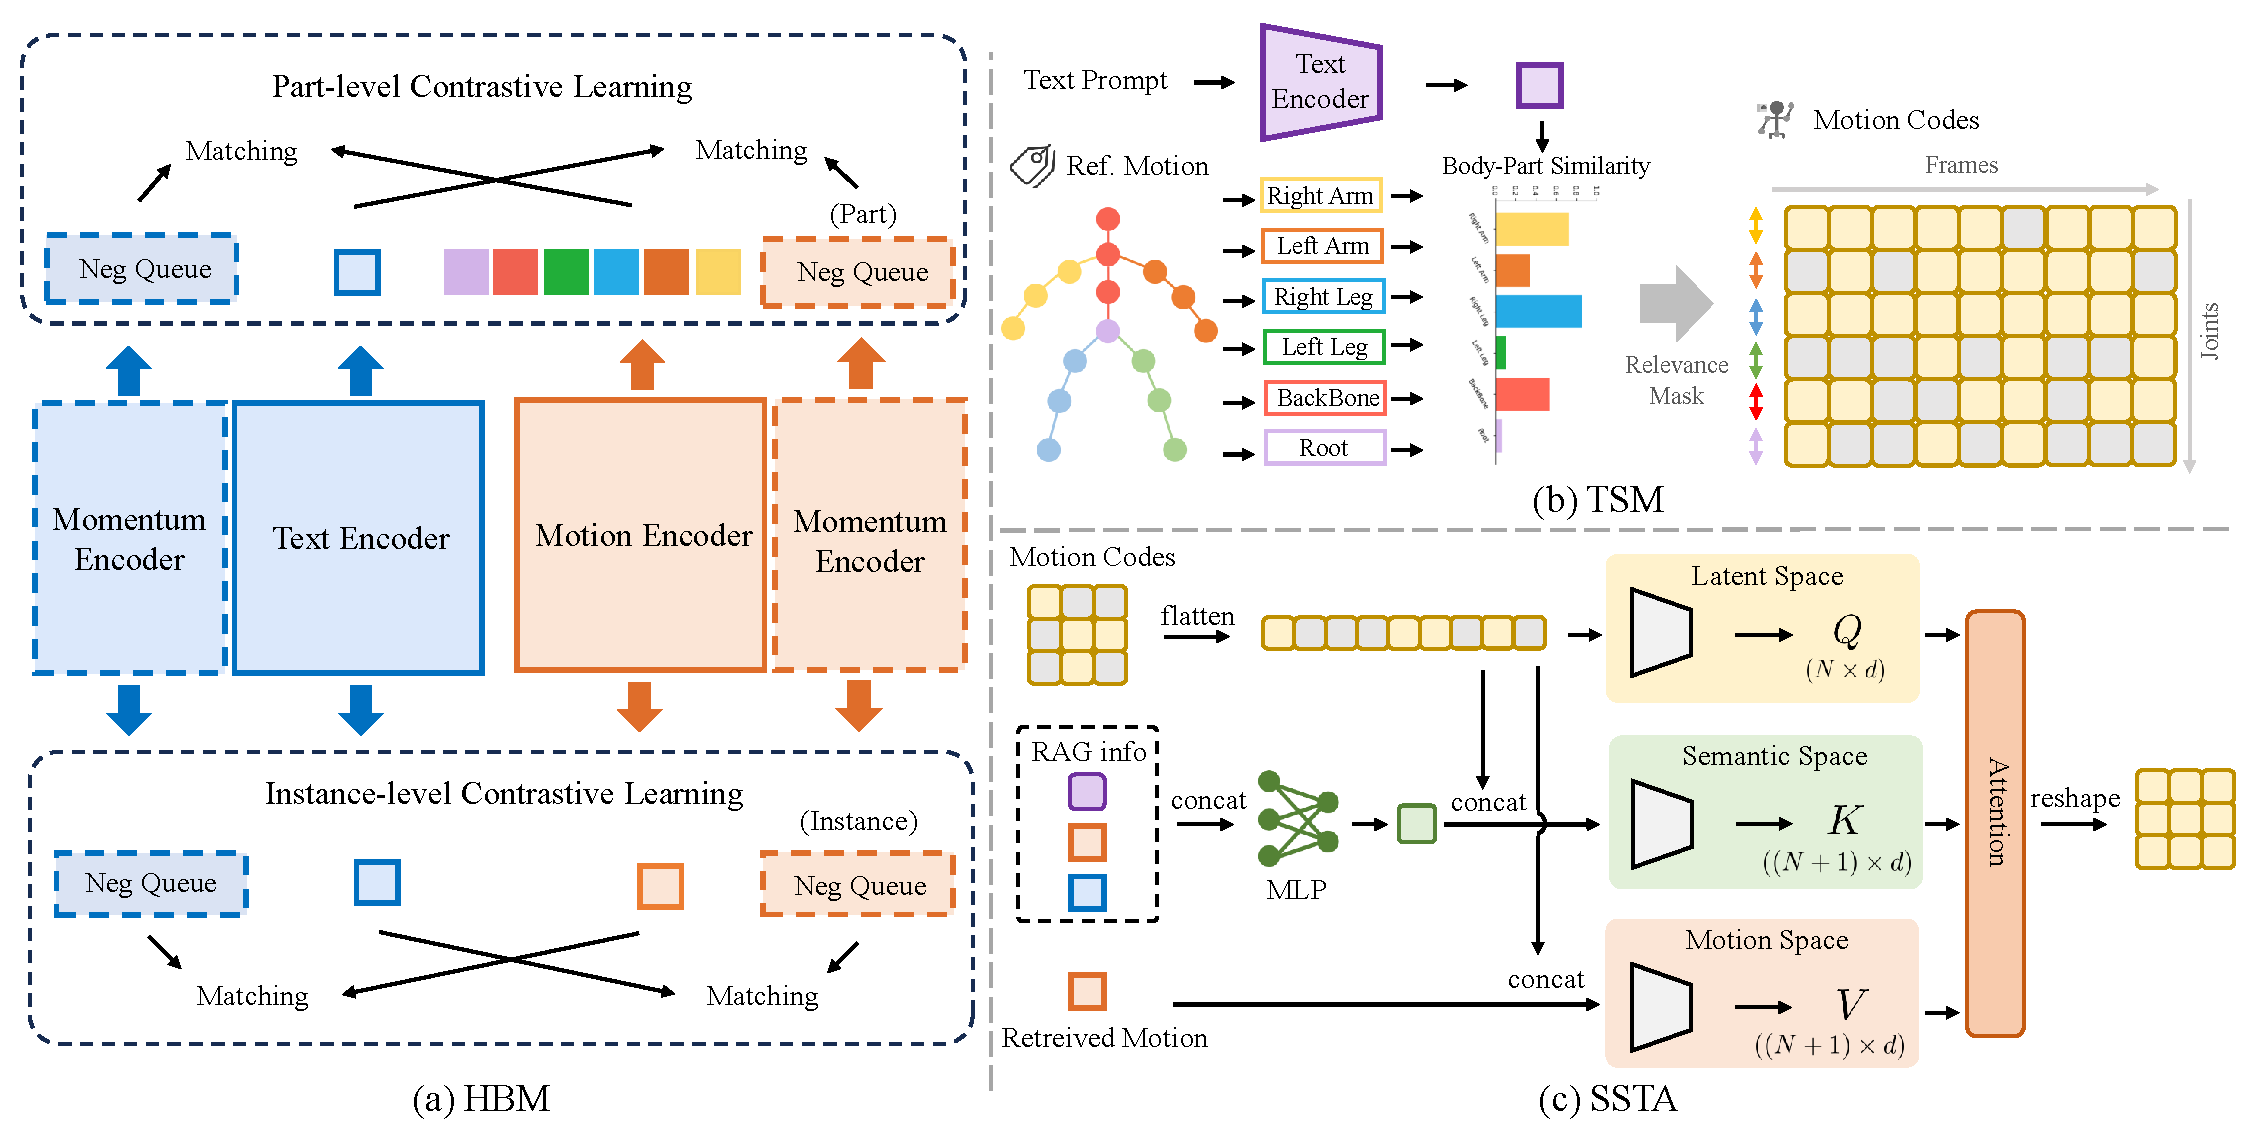
\includegraphics[width=\textwidth]{fig/framework.pdf} 
%     \caption{\textbf{Framework of ReMoMask.} 
%     (a) \textbf{H}ierarchical \textbf{B}idirectional \textbf{M}omentum (HBM) learning, which constructs a structured embedding space via instance-level and part-level bidirectional contrastive alignment using momentum encoders and negative queues. 
%     (b) \textbf{T}opology \textbf{S}tructured \textbf{M}asking (TSM), which computes body-part similarity scores from the HBM space to generate an adaptive relevance mask, forcing the model to focus on reconstructing semantically deficient regions. 
%     (c) \textbf{S}emantic \textbf{S}patial--\textbf{T}emporal \textbf{A}ttention (SSTA), which injects retrieved semantic information into the generation process via an asymmetric Q-K-V design, where semantics modulate attention weights (Key) while motion topology is preserved in the content synthesis (Query/Value).
%     }
%     %     \label{fig:framework}
% \end{figure*}



\begin{figure*}[t] 
    \centering 
    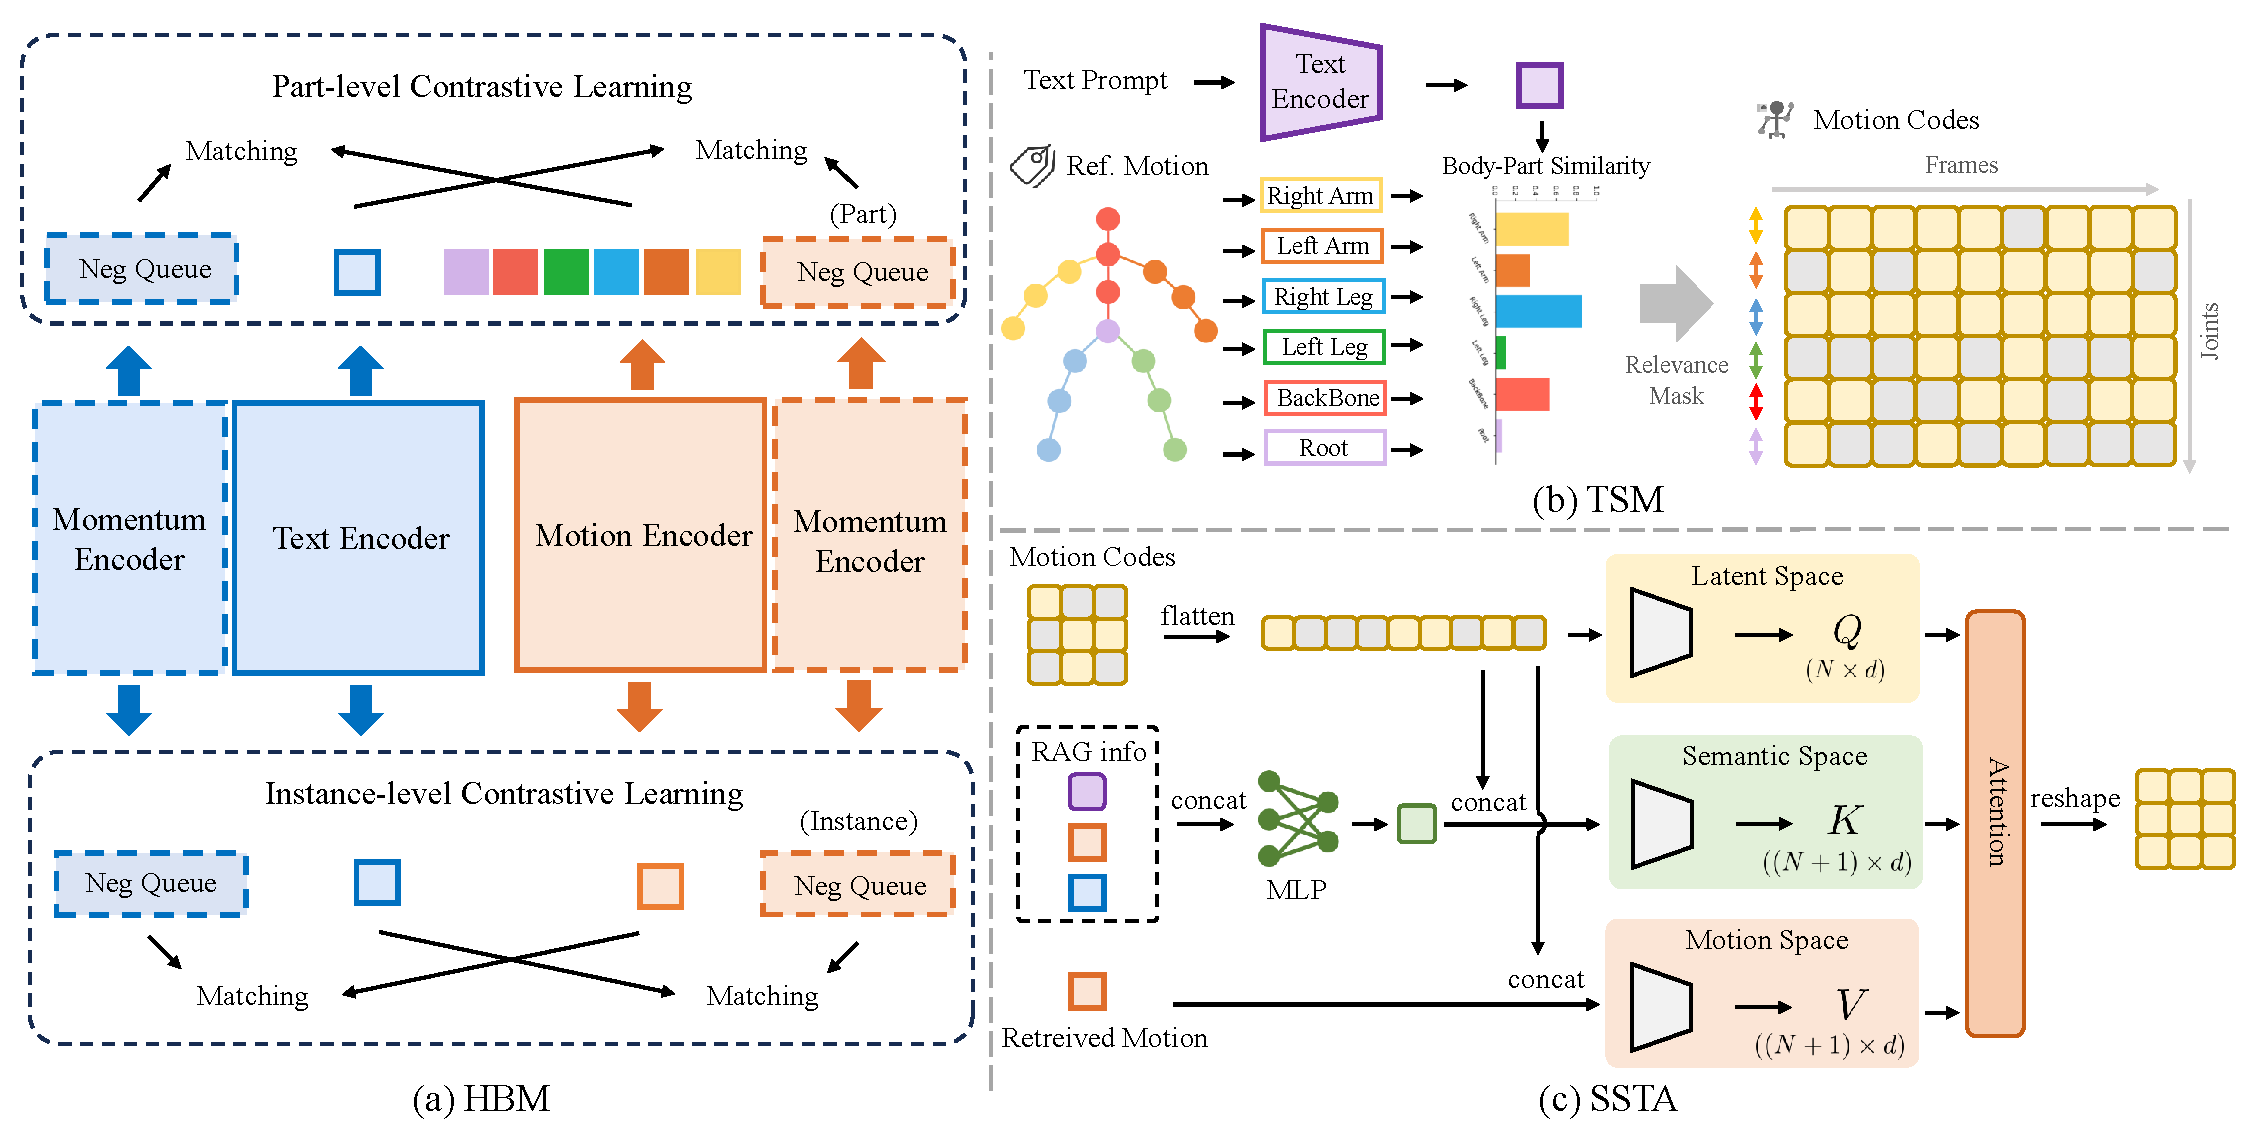
\includegraphics[width=\textwidth]{fig/framework.pdf} 
    \caption{\textbf{Framework of ReMoMask.} 
    (a) \textbf{H}ierarchical \textbf{B}idirectional \textbf{M}omentum (HBM): Constructs a structured embedding space via instance and part level contrastive alignment with momentum encoders. 
    (b) \textbf{T}opology \textbf{S}tructured \textbf{M}asking (TSM): Generates adaptive masks based on body-part similarity to prioritize reconstructing semantically deficient regions. 
    (c) \textbf{S}emantic \textbf{S}patial--\textbf{T}emporal \textbf{A}ttention (SSTA): Injects retrieved semantics via an asymmetric Q-K-V design, where semantics modulate attention (Key) while motion topology is preserved in synthesis (Query/Value).
    }
        \label{fig:framework}
\end{figure*}


As illustrated in Fig.~\ref{fig:teaser}, our framework follows a retrieval-augmented generation paradigm. We first employ \textbf{Hierarchical Bidirectional Momentum (HBM)} learning to align text and motion at both instance and part levels, constructing a hierarchically organized embedding space for accurate retrieval. During training, we utilize \textbf{Topology Structured Masking (TSM)}, a structure-aware masked modeling objective that adaptively modulates masking probabilities based on hierarchical relevance to strengthen part-level grounding. Given an input text prompt $x$, relevant motion-text pairs are retrieved from this structured space to obtain reference embeddings ($R_m, R_t$), which are then injected into the generator via our proposed \textbf{Semantic Spatial--Temporal Attention (SSTA)} to enable topology-aware semantic conditioning over 2D motion tokens.

In this pipeline, retrieval operates in the contrastive semantic space constructed by HBM, whereas generation operates on the latents of a 2D RVQ-VAE---two representations learned under disjoint objectives. Sections~\ref{subsec:lar} and~\ref{subsec:vroute} present the extension that defines \textbf{ReMoMask-2}: we migrate retrieval into the generator's own pre-quantization latent space, and on this basis revisit a value-pathway routing decision of SSTA whose premise this migration changes.

%%%%%%%%%%%%%%%%
\subsection{Hierarchical Bidirectional Momentum}
\label{subsec:hbm}
\noindent \myparagraph{Hierarchical Motion Decomposition.}
As shown in Fig.~\ref{fig:framework}b, we decompose motion $m$ into $K=6$ semantic parts (e.g., arms, legs, backbone, root), denoted as $m^k$. Given a batch $\{(x_i, m_i)\}_{i=1}^{B}$, we encode text, global motion, and part motions into a shared space:
\begin{equation}
t_i = f_T(x_i), \quad
g_i = f_G(m_i), \quad
p_{i,k} = f_P^{(k)}(m_i^k),
\end{equation}
where $f_T$, $f_G$, and $f_P^{(k)}$ are the respective encoders.

\noindent \myparagraph{Momentum-Based Structured Contrast.}
To stabilize training and enlarge the negative set, we maintain momentum encoders with parameters updated via exponential moving average:
\begin{equation}
\theta^{-} \leftarrow \mu\, \theta^{-} + (1 - \mu)\, \theta,
\end{equation}
where $\theta$ and $\theta^{-}$ denote online and momentum parameters. The resulting momentum embeddings ($t_i^{-}, g_i^{-}, p_{i,k}^{-}$) are stored in a queue $\mathcal{Q}$ serving as negative keys.

\noindent \myparagraph{Contrastive Objective.}
Using cosine similarity $\mathrm{sim}(\cdot,\cdot)$ and temperature $\tau$, we define the positive term $\mathcal{P}(q,k) = \exp(\mathrm{sim}(q,k)/\tau)$ and negative sum $\mathcal{N}(q) = \sum_{k^- \in \mathcal{Q}} \exp(\mathrm{sim}(q,k^-)/\tau)$. The InfoNCE loss is:
\begin{equation}
\mathrm{InfoNCE}(q,k)
=
-\log
\frac{
    \mathcal{P}(q,k)
}{
    \mathcal{P}(q,k) + \mathcal{N}(q)
}.
\end{equation}

\noindent \myparagraph{Bidirectional Alignment.}
We enforce bidirectional alignment at the instance level:
\begin{equation}
\mathcal{L}_{\mathrm{Inst}}
=
\frac{1}{B}
\sum_{i=1}^{B}
\Big(
\mathrm{InfoNCE}(t_i, g_i)
+
\mathrm{InfoNCE}(g_i, t_i)
\Big),
\end{equation}
and further align text with each part representation to preserve fine-grained semantics:
\begin{equation}
\mathcal{L}_{\mathrm{Part}}
=
\frac{1}{BK}
\sum_{i=1}^{B}
\sum_{k=1}^{K}
\Big(
\mathrm{InfoNCE}(t_i, p_{i,k})
+
\mathrm{InfoNCE}(p_{i,k}, t_i)
\Big).
\end{equation}

\noindent \myparagraph{Final Objective.}
The total HBM loss combines global and part-level supervision:
\begin{equation}
\mathcal{L}_{\mathrm{HBM}}
=
\mathcal{L}_{\mathrm{Inst}}
+
\lambda_P \mathcal{L}_{\mathrm{Part}}.
\end{equation}
This hierarchical supervision yields a structurally consistent embedding space for precise retrieval.

%%%%%%%%%%%%%%%%%%%%%

\subsection{Part-Level Motion Encoder} 
\label{app:part-level-motion-encoder}
\begin{figure}[t!]
    \centering
     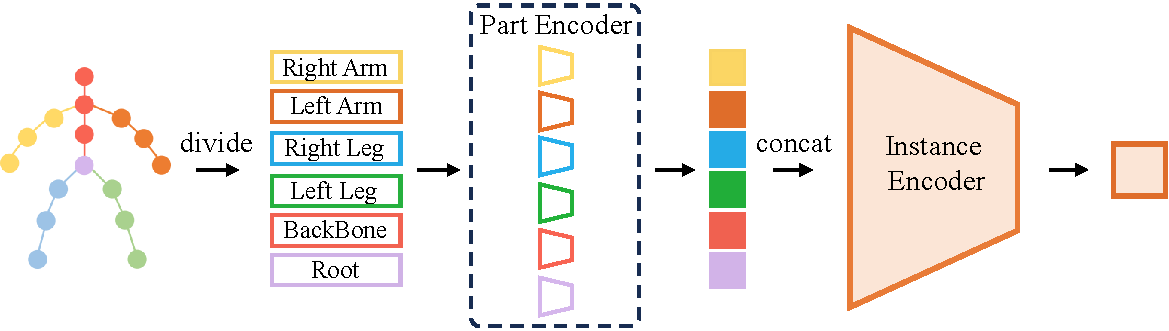
\includegraphics[width=\linewidth]{fig/part-level-motion-encoder.pdf}
    \caption{\textbf{Part-level motion encoding for hierarchical alignment.} 
    The full-body motion sequence is first divided into multiple body parts according to the skeletal structure. Each part motion is encoded independently by a shared part encoder to obtain part-level features, which are then concatenated and aggregated by an instance encoder to produce a global motion representation. This hierarchical encoding enables fine-grained part-level semantics while preserving holistic motion information.}
    \label{fig:part-level-motion-encoder}
\end{figure}
To capture the hierarchical structure of human motion, inspired by prior human motion modeling works~\cite{parco,remogpt}, we adopt a part-level motion encoding scheme that decomposes full-body motion into multiple semantically meaningful body parts. As illustrated in Fig.~\ref{fig:part-level-motion-encoder}, a motion sequence is first divided into six parts according to the skeletal topology, including the right arm, left arm, right leg, left leg, backbone, and root. Each part motion is processed independently by a shared part encoder to obtain part-level motion features. These features preserve fine-grained local motion semantics while maintaining parameter efficiency through weight sharing. The resulting part-level representations are then concatenated and aggregated by an instance encoder to form a holistic motion representation, which is subsequently used for hierarchical alignment and retrieval. This hierarchical encoding design enables the model to jointly model local part dynamics and global motion coherence, providing a structured motion representation that facilitates fine-grained text--motion alignment in the proposed framework.

\subsection{Topology Structured Masking}
\label{subsec:tsm}

To fully exploit the hierarchical structure learned by HBM during generation, we introduce \textbf{Topology Structured Masking (TSM)} as a structure-aware training objective. Unlike conventional uniform random masking that ignores semantic relevance, TSM adaptively modulates masking probabilities based on the hierarchical text--motion alignment established by HBM, ensuring the generator focuses on semantically critical body parts.

\noindent \myparagraph{Hierarchical Semantic Relevance.}
As shown in Fig.~\ref{fig:framework}b, given a text embedding $t_i$ and part-level motion embeddings $\{p_{i,k}\}_{k=1}^{K}$ from HBM, we compute part-level relevance weights:
\begin{equation}
\alpha_{i,k}
=
\mathrm{SoftMax}_k
\big(
\mathrm{sim}(t_i, p_{i,k})
\big),
\end{equation}
where $\alpha_{i,k}$ reflects the semantic alignment strength between the input text and the $k$-th body part.


\noindent \myparagraph{Topology-Aware Mask Distribution.}
We define the masking probability for each body part as:
\begin{equation}
\pi_{i,k}
=
\pi_{\mathrm{base}}
\cdot
(1 - \alpha_{i,k}),
\end{equation}
where $\pi_{\mathrm{base}}$ is a global masking ratio. This strategy ensures that semantically aligned parts are preserved as structural anchors, while less relevant parts are masked aggressively. By protecting these core semantic features from corruption, we force the generator to learn how to coordinate global motion conditioned on the key body parts specified by the text, rather than attempting to hallucinate critical semantics from context. These part-level probabilities are then propagated to the 2D spatial--temporal token grid ($J \times T$) according to the skeletal partition, such that all joints belonging to part $k$ share the probability $\pi_{i,k}$.

\noindent \myparagraph{Structured Masked Modeling Objective.}
During training, tokens are masked according to $\pi_{i,k}$ and replaced by a learnable mask token. The generator is optimized to reconstruct the original latent codes $z$:
\begin{equation}
\mathcal{L}_{\mathrm{TSM}}
=
\mathbb{E}_{z}
\left[
\| z_{\mathrm{pred}} - z \|_{\mathrm{masked}}
\right].
\end{equation}
By aligning the masking distribution with semantic relevance, TSM forces the model to focus on reconstructing critical body parts, thereby enhancing part-level grounding and structural consistency.




%%%%%%%%%%%%%%%%%%%
\subsection{Semantic Spatial-Temporal Attention}
\label{subsec:ssta}
% While hierarchical retrieval provides structured embeddings, effective generation requires injecting these semantics in a manner consistent with motion topology. 
Unlike conventional cross-attention that treats retrieved features as uniform tokens, we design \textbf{Semantic Spatial--Temporal Attention (SSTA)} to explicitly respect the 2D spatial–temporal organization of motion latents through an asymmetric injection mechanism.

We represent motion as a 2D joint–time token grid, flattened into latent sequences $z \in \mathbb{R}^{B \times N \times d}$ (where $N = T \cdot J$). As illustrated in Fig.~\ref{fig:framework}(c), SSTA decouples the roles of semantic conditioning and motion synthesis across the Key and Value pathways.

\noindent \myparagraph{Query: Motion-Centric Focus.}
To preserve the structural integrity of the generation process, the Query is derived solely from the current motion latents:
\begin{equation}
Q = W_q z,
\end{equation}
ensuring that attention computation remains anchored in the spatial–temporal topology of the motion being generated.

\noindent \myparagraph{Semantic Reference Construction.}
We compress the multi-modal retrieval context (prompt $t$, retrieved text $R_t$, and retrieved motion $R_m$) into a compact semantic token:
\begin{equation}
h_{\mathrm{sem}} = \mathrm{MLP}\!\left(
\mathrm{concat}[t;\, R_t;\, R_m]
\right),
\end{equation}
where $h_{\mathrm{sem}} \in \mathbb{R}^{B \times 1 \times d}$ serves as a global modulation signal rather than a sequence of tokens.

\noindent \myparagraph{Key: Topology-Aware Gating.}
The Key pathway integrates both motion states and semantic context to determine \emph{where} to attend:
\begin{equation}
K = W_k \cdot
\mathrm{concat}\!\left(z,\; h_{\mathrm{sem}}\right).
\end{equation}
By injecting $h_{\mathrm{sem}}$ only into the Key, semantic information modulates the attention weights without directly overwriting the motion representation.

\noindent \myparagraph{Value: Motion-Domain Synthesis.}
The Value pathway focuses on \emph{what} information to synthesize, combining current latents with retrieved dynamic priors:
\begin{equation}
V = W_v \cdot
\mathrm{concat}\!\left(z,\; R_m\right).
\end{equation}
Here, $R_m$ provides concrete motion details from the database, while $z$ ensures continuity with the current generation state. Notably, textual semantics ($t, R_t$) are excluded from Value to prevent domain mismatch; Section~\ref{subsec:vroute} revisits this choice for $R_t$ in ReMoMask-2, where latent alignment turns $R_t$ into a motion-domain signal.

\noindent \myparagraph{Output.}
The final output is computed via standard scaled dot-product attention:
\begin{equation}
\mathrm{Output}
=
\mathrm{SoftMax}
\left(
    \frac{QK^\top}{\sqrt{d}}
\right)V,
\end{equation}
which is then reshaped back to the 2D grid structure. This asymmetric design ensures that retrieved semantics guide the attention focus (via Key) and enrich the motion content (via $R_m$ in Value), while strictly preserving the spatial–temporal topology of the generative backbone.


%%%%%%%%%%%%%%%%%%%
\subsection{Latent-Aligned Retrieval}
\label{subsec:lar}

The components above enforce structural consistency along the two axes identified in Section~\ref{sec:introduction}: HBM aligns text and motion at the granularity dictated by skeletal topology, and SSTA injects retrieved evidence in a form compatible with the 2D spatial--temporal latent grid. A third axis, however, remains open. In ReMoMask---as in retrieval-augmented T2M at large~\cite{remodiffuse,remogpt,morag}---the space in which evidence is \emph{retrieved} is not the space in which motion is \emph{generated}: HBM embeds text and motion into a contrastive space $\mathcal{S} \subset \mathbb{R}^{512}$, optimized by InfoNCE to discriminate matching from non-matching pairs, whereas the masked generator operates on the latent space $\mathcal{Z}$ of the 2D RVQ-VAE, optimized purely for reconstruction. Retrieval evidence $(R_m, R_t) \in \mathcal{S}$ is therefore consumed by attention layers whose substrate lives in $\mathcal{Z}$: implicitly, the fusion modules are asked to realize a cross-space translation $\psi: \mathcal{S} \rightarrow \mathcal{Z}$, supervised only indirectly through the generation loss. Since the two spaces never interact during training, nothing constrains their geometries to agree---two motions that are close under contrastive semantics may be far apart as latent trajectories. We refer to this discrepancy as the \emph{retrieval--generation representation gap}.

ReMoMask-2 removes the gap at its source: rather than translating evidence across spaces, we construct the retrieval database directly in the generator's own latent space, so that retrieved evidence arrives, by construction, in the representation the generator natively consumes.

\noindent \myparagraph{Pre-Quantization Latent Keys.}
We build retrieval keys with the frozen encoder $\mathcal{E}$ of the pretrained 2D RVQ-VAE~\cite{mogents}. Given a motion $m$, the encoder produces a pre-quantization latent grid
\begin{equation}
z_e = \mathcal{E}(m) \in \mathbb{R}^{d_e \times T' \times J'},
\end{equation}
with channel dimension $d_e = 1024$ over a downsampled grid of $T' = T/4$ temporal steps and $J' = 6$ spatial positions. We deliberately operate on the continuous latent \emph{before} residual quantization rather than on discrete token indices: the pre-quantization latent preserves the continuous geometry of the encoder space and directly supports cosine-based nearest-neighbor search, whereas quantized indices are categorical and discard within-code variation. A motion-level key is obtained by average pooling over the grid followed by $\ell_2$ normalization:
\begin{equation}
\bar{z}_e
=
\frac{\hat{z}_e}{\|\hat{z}_e\|_2},
\qquad
\hat{z}_e
=
\frac{1}{T' J'}
\sum_{t'=1}^{T'}
\sum_{j'=1}^{J'}
z_e(t', j'),
\end{equation}
where $z_e(t', j') \in \mathbb{R}^{d_e}$ denotes the latent vector at grid position $(t', j')$. Applying this to every training motion and expanding each motion over its captions yields the database
\begin{equation}
\mathcal{D}
=
\big\{ \big( \bar{z}_e^{(j)},\, x^{(j)} \big) \big\}_{j=1}^{M},
\qquad
M = 66{,}912,
\end{equation}
covering the 23{,}384 sequences of the mirror-augmented HumanML3D training split; at query time, entries originating from the same motion are deduplicated so that the retrieved set contains distinct exemplars. Since keys are unit-normalized, retrieval reduces to cosine similarity over $\mathcal{D}$. The RVQ-VAE remains entirely frozen throughout---the database is a cached view of representations the generator already uses.

\noindent \myparagraph{Query Projector.}
Retrieval requires mapping a text prompt into the same key space. We instantiate this as a lightweight projector $\phi$ applied to the 512-d CLIP ViT-B/32~\cite{clip} text embedding $t$ already employed by the framework:
\begin{equation}
\phi(t)
=
\mathrm{norm}\big( W_2\, \mathrm{GELU}( W_1 t ) \big),
\end{equation}
where $W_1 \in \mathbb{R}^{1024 \times 512}$, $W_2 \in \mathbb{R}^{1024 \times 1024}$, and $\mathrm{norm}(\cdot)$ denotes $\ell_2$ normalization. The projector holds ${\sim}1.57$M parameters and is the \emph{only} component trained in this stage.

\noindent \myparagraph{Distillation from the HBM Retriever.}
Naively regressing $\phi(t)$ onto the paired key would supervise a single point and ignore the ranking structure that makes retrieval useful. Instead, we distill the HBM retriever of the conference version---which remains a strong cross-modal ranker---into the latent key space.
% TODO-CITE: Hinton et al., "Distilling the Knowledge in a Neural Network" (soft-target knowledge distillation), for the distillation formulation.
For a training caption $x$ with embedding $t$, let $\Omega(x)$ denote the $\kappa$ database entries ranked highest by the teacher ($\kappa = 256$). Teacher and student induce distributions over $\Omega(x)$ from their respective similarities at temperature $\tau = 0.07$, matching the retriever's contrastive temperature:
\begin{equation}
p^{\square}_j
=
\frac{
    \exp\big( s^{\square}_j / \tau \big)
}{
    \sum_{j' \in \Omega(x)} \exp\big( s^{\square}_{j'} / \tau \big)
},
\qquad
\square \in \{ \mathrm{HBM}, \phi \},
\end{equation}
where $s^{\mathrm{HBM}}_j$ is the teacher's text--motion similarity for entry $j$ in $\mathcal{S}$, and $s^{\phi}_j = \mathrm{sim}\big( \phi(t), \bar{z}_e^{(j)} \big)$ is the student's cosine similarity in the latent key space. The projector minimizes the KL divergence from teacher to student,
\begin{equation}
\mathcal{L}_{\mathrm{align}}
=
\mathrm{KL}\big( p^{\mathrm{HBM}} \,\|\, p^{\phi} \big)
=
\sum_{j \in \Omega(x)}
p^{\mathrm{HBM}}_j
\log
\frac{p^{\mathrm{HBM}}_j}{p^{\phi}_j}.
\end{equation}
Restricting the support to the teacher's top-$\kappa$ candidates concentrates supervision on the ranking decisions that matter for retrieval, and the soft targets transfer the teacher's graded preferences rather than a single hard label. The projector is trained for 200 epochs with a batch size of 128, while the RVQ-VAE, the teacher, and the CLIP text encoder all remain frozen. In effect, distillation transfers the teacher's cross-modal ranking into the generative latent space: the resulting retriever inherits the semantic precision of HBM while returning evidence natively expressed in the generator's representation.

\noindent \myparagraph{Integration with SSTA.}
At generation time, the query $\phi(t)$ retrieves the nearest database entries by cosine similarity, and both retrieval streams are read out of the latent-aligned space: $R_m$ is the pooled key $\bar{z}_e^{(j)}$ of a retrieved entry, and $R_t = \phi(t^{(j)})$ is the projection of the CLIP embedding $t^{(j)}$ of its caption $x^{(j)}$. As both streams are $d_e$-dimensional while the generator operates at latent width $d$, we insert two linear adapters, $\mathbb{R}^{d_e} \rightarrow \mathbb{R}^{d}$, one per stream, ahead of the fusion pathways. These adapters are the only architectural addition: SSTA itself---the asymmetric Q-K-V routing of Section~\ref{subsec:ssta}, including the three-way semantic token $h_{\mathrm{sem}} = \mathrm{MLP}(\mathrm{concat}[t;\, R_t;\, R_m])$---is left unchanged. Latent-aligned retrieval is thus a plug-and-play replacement for the retrieval space, and any improvement it yields is attributable to \emph{where} the evidence lives, not to additional fusion capacity.

%%%%%%%%%%%%%%%%%%%
\subsection{Revisiting Value-Pathway Routing}
\label{subsec:vroute}

The conference version routes retrieval evidence asymmetrically through SSTA: the semantic token $h_{\mathrm{sem}}$, carrying $t$, $R_t$, and $R_m$, modulates the Key, while the Value admits only motion-domain content, $V = W_v \cdot \mathrm{concat}(z, R_m)$. Textual signals were deliberately excluded from the Value pathway because, in that design, $R_t$ is an embedding in the contrastive semantic space $\mathcal{S}$: injecting a cross-domain vector into the pathway that directly synthesizes motion content risks contaminating the output with non-motion statistics, and the information-source ablation (Table~\ref{tab:ablation}) confirmed, under the conference protocol, that admitting the semantic-space $R_t$ into the Value degrades fidelity. Under that premise, the routing embodies a sound principle---\emph{Value content should stay in the motion domain}.

Latent alignment changes the premise, not the principle. In ReMoMask-2, $R_t = \phi(t^{(j)})$ is distilled into the $z_e$-aligned key space: it is no longer a foreign semantic vector but the caption's projection onto the generator's own latent geometry---in effect, a text-anchored motion prior. The domain-mismatch rationale for excluding $R_t$ from the Value therefore no longer applies to it, and we re-open the routing accordingly:
\begin{equation}
V = W_v \cdot
\mathrm{concat}\!\left(z,\; R_m,\; R_t\right),
\end{equation}
at zero architectural cost: $R_m$ continues to supply exemplar dynamics from a specific retrieved motion, while $R_t$ contributes a smoother, caption-conditioned estimate of where in latent space the described motion should lie. The Query and Key pathways are unchanged, and the prompt embedding $t$---which still resides in the CLIP semantic space---remains excluded from the Value: the criterion that the Value pathway admit only motion-domain signals is preserved, and what has changed is that, after latent alignment, $R_t$ satisfies it.

We treat this routing update as an independent, minor contribution, orthogonal to latent-aligned retrieval itself. Because it re-examines a conclusion of the conference ablation under a changed premise, we verify it explicitly with a $2{\times}2$ ablation (Table~\ref{tab:ablation_v2_orthogonal}) that crosses the retrieval space (semantic vs.\ latent-aligned) with the routing (with vs.\ without $R_t$ in the Value); enabling the route under latent-aligned retrieval improves FID by \textbf{[TBD]}.


\section{Experiment}
\label{sec:experiment}
% \begin{table}[t]
\begin{table*}[t!]
\centering
\caption{\textbf{Results of text-to-motion and motion-to-text retrieval benchmark on HumanML3D, KIT-ML, and SnapMoGen datasets.}
$\dagger$ indicates Results are reproduced by us following the descriptions in the original paper, as no official implementation is publicly available. Best results are highlighted in \textbf{bold}, and second-best results are \underline{underlined}.}
\label{tab:rag_experiment} 
% \setlength{\tabcolsep}{4pt}  % Adjust the column spacing
% \small % Adjust the font size
% \setlength{\tabcolsep}{3.5pt}  % Adjust the column spacing
\resizebox{\textwidth}{!}{
    \begin{tabular}{l|l|cccccc|cccccc}
        \toprule
        \multirow{2}{*}{Benchmark} & \multirow{2}{*}{Methods} 
        & \multicolumn{6}{c|}{Text-to-motion retrieval} 
        & \multicolumn{6}{c}{Motion-to-text retrieval} \\
        & 
        & R@1$\uparrow$ & R@2$\uparrow$ & R@3$\uparrow$ & R@5$\uparrow$ & R@10$\uparrow$ & MedR$\downarrow$
        & R@1$\uparrow$ & R@2$\uparrow$ & R@3$\uparrow$ & R@5$\uparrow$ & R@10$\uparrow$ & MedR$\downarrow$ \\
        \hline\hline
        
        \multirow{6}{*}{HumanML3D}
        & TEMOS~\cite{temos}
        & 2.12 & 4.09 & 5.87 & 8.26 & 13.52 & 173.00
        & 3.86 & 4.54 & 6.94 & 9.38 & 14.00 & 183.25 \\
        & TMR~\cite{tmr}
        & 5.68 & 10.59 & 14.04 & 20.34 & 30.94 & 28.00
        & 9.95 & 12.44 & 17.95 & 23.56 & 32.69 & 28.50 \\
        & MotionPatches$^{\dag}$~\cite{motionpatches}
        & 10.80 & 14.98 & 20.00 & 26.72 & 38.02 & 19.00
        & 11.25 & 13.86 & 19.98 & 26.86 & 37.40 & 20.50 \\
        & ReMoGPT$^{\dag}$~\cite{remogpt}
        & \underline{11.00} & \underline{17.02} & \underline{22.18} & \underline{29.48} & \underline{43.43} & \underline{14.00}
        & \underline{12.25} & \underline{14.95} & \underline{21.45} & \underline{28.34} & \underline{39.11} & \underline{19.00} \\
        \rowcolor[gray]{0.90} \cellcolor{white} & HBM (ReMoMask)
        & \textbf{18.49} & \textbf{21.20} & \textbf{25.63} & \textbf{32.40} & \textbf{46.27} & \textbf{12.00}
        & \textbf{14.83} & \textbf{17.63} & \textbf{25.60} & \textbf{30.75} & \textbf{44.61} & \textbf{16.00} \\
        \rowcolor{yellow!20} \cellcolor{white} & \textbf{ReMoMask-2}
        & xx.xx & xx.xx & xx.xx & xx.xx & xx.xx & xx.xx
        & xx.xx & xx.xx & xx.xx & xx.xx & xx.xx & xx.xx \\
        \midrule

        \multirow{6}{*}{KIT-ML}
        & TEMOS~\cite{temos}
        & 7.11 & 13.25 & 17.59 & 24.10 & 35.66 & 24.00
        & 11.69 & 15.30 & 20.12 & 26.63 & 36.39 & 26.50 \\
        & TMR~\cite{tmr}
        & 7.23 & 13.98 & 20.36 & 28.31 & 40.12 & 17.00
        & 11.20 & 13.86 & 20.12 & 28.07 & 38.55 & 18.00 \\
        & MotionPatches$^{\dag}$~\cite{motionpatches}
        & \underline{14.02} & \underline{21.08} & \underline{28.91} & \underline{34.10} & \underline{50.00} & \underline{10.50}
        & \textbf{13.61} & \textbf{17.26} & \textbf{27.54} & \underline{33.33} & \underline{44.77} & \textbf{13.00} \\
        & ReMoGPT$^{\dag}$~\cite{remogpt}
        & 13.42 & 17.65 & 22.24 & 32.30 & 44.68 & 12.50
        & 11.93 & 14.12 & 21.59 & 30.54 & 39.68 & 16.50 \\
        \rowcolor[gray]{0.90} \cellcolor{white} & HBM (ReMoMask)
        & \textbf{16.75} & \textbf{23.10} & \textbf{30.50} & \textbf{37.56} & \textbf{52.20} & \textbf{8.50}
        & \underline{12.14} & \underline{16.36} & \underline{25.64} & \textbf{35.58} & \textbf{46.15} & \underline{14.00} \\
        \rowcolor{yellow!20} \cellcolor{white} & \textbf{ReMoMask-2}
        & xx.xx & xx.xx & xx.xx & xx.xx & xx.xx & xx.xx
        & xx.xx & xx.xx & xx.xx & xx.xx & xx.xx & xx.xx \\
        \midrule

        \multirow{6}{*}{SnapMoGen}
        & TEMOS~\cite{temos} & 5.03 & 8.51 & 10.79 & 14.48 & 20.36 & 42.00
        & 4.72 & 6.67 & 7.95 & 10.11 & 16.74 & 64.00 \\
        & TMR~\cite{tmr} & 7.29 & 11.80 & 14.43 & 18.82 & 27.39 & 28.50
        & 8.03 & 10.22 & 13.49 & 20.91 & 29.06 & 33.00 \\
        & MotionPatches$^{\dag}$~\cite{motionpatches} & \underline{8.92} & \underline{14.75} & \underline{18.13} & \underline{25.46} & \underline{34.95} & \underline{19.00}
        & 9.08 & 12.24 & 14.73 & 22.42 & 33.52 & 25.50 \\
        & ReMoGPT$^{\dag}$~\cite{remogpt} & 8.15 & 13.27 & 16.05 & 24.72 & 33.48 & 20.50 
        & \underline{9.94} & \underline{13.55} & \underline{16.41} & \underline{23.87} & \underline{35.53} & \underline{23.00} \\
        \rowcolor[gray]{0.90} \cellcolor{white} & HBM (ReMoMask) & \textbf{12.43} & \textbf{17.84} & \textbf{22.54} & \textbf{28.22} & \textbf{42.83} & \textbf{16.50}
        & \textbf{11.62} & \textbf{15.35} & \textbf{19.32} & \textbf{26.18} & \textbf{39.41} & \textbf{19.00} \\
        \rowcolor{yellow!20} \cellcolor{white} & \textbf{ReMoMask-2}
        & xx.xx & xx.xx & xx.xx & xx.xx & xx.xx & xx.xx
        & xx.xx & xx.xx & xx.xx & xx.xx & xx.xx & xx.xx \\
        \bottomrule
    \end{tabular}
}
\end{table*}
% \end{table}




\begin{table*}[t]
    \centering
    \caption{\textbf{Quantitative evaluation on HumanML3D, KIT-ML, and SnapMoGen datasets.} We repeat the evaluation 20 times and report the average with 95\% confidence interval. Results marked with $\dagger$ are reproduced following the original paper, as no official implementation is publicly available. \textbf{Bold} and \underline{underline} indicate the best and the second best results.}
    \label{tab:t2m_experiment} 
    % \renewcommand{\arraystretch}{1.1}  % Adjust the line height (global)
    % \small % Adjust the font size
    % \setlength{\tabcolsep}{3.5pt}  % Adjust the column spacing
    % \vspace{-0.5em}
    \resizebox{\textwidth}{!}{
    \begin{tabular}{l|l| c | c c c| c |c| c| c}
        \toprule
          & \multirow{2}{*}{Methods} & \multirow{2}{*}{Framework}  & \multicolumn{3}{c|}{R-Precision$\uparrow$} & \multirow{2}{*}{FID$\downarrow$} & \multirow{2}{*}{MMDIST$\downarrow$} & \multirow{2}{*}{Diversity$\rightarrow$} & \multirow{2}{*}{MModality$\uparrow$}\\
        \cline{4-6}
           ~& ~ & ~& Top 1 & Top 2 & Top 3 & & & & \\

        % humanml3d
        \hline\hline 
        \rule{0pt}{2.5ex} % Adjust the line height (local)
        \multirow{14}{*}{\rotatebox{90}{\textbf{HumanML3D}}} &
        Real & - & $0.511^{\pm.003}$ & $0.703^{\pm.003}$  & $0.797^{\pm.002}$ &$0.002^{\pm0.000}$ & $2.974^{\pm0.008}$& $9.503^{\pm0.065}$ & $-$ \\
        \cmidrule{2-10}
        & MDM~\cite{mdm} & \multirow{7}{*}{t2m} & $-$ & $-$  & $0.611^{\pm.007}$ &$0.544^{\pm0.44}$ & $5.566^{\pm.027}$& $9.559^{\pm.086}$ & $2.799^{\pm.072}$ \\
        & T2M-GPT~\cite{t2m-gpt} & &$0.492^{\pm.003}$&$0.679^{\pm.002}$&$0.775^{\pm.002}$&$0.141^{\pm.005}$&$3.121^{\pm.009}$& $9.761^{\pm.073}$ & $1.856^{\pm.003}$ \\ 
        & MoMask~\cite{momask} & &$0.521^{\pm.002}$ & $0.713^{\pm.002}$  &$0.807^{\pm.002}$ & $0.045^{\pm.002}$ &$2.958^{\pm.008}$& $9.589^{\pm.035}$ & $1.241^{\pm.040}$\\
        & MoGenTS~\cite{mogents} & &$0.529^{\pm.003}$ & $0.719^{\pm.002}$& $0.812^{\pm.002}$& $0.033^{\pm.001}$ & $2.867^{\pm.006}$& $9.570^{\pm.077}$ & $1.205^{\pm.043}$\\
        & MoMask++~\cite{momask2} & &$0.517^{\pm.002}$  &$0.709^{\pm.002}$ &$0.803^{\pm.002}$ &$0.069^{\pm.003}$&$2.948^{\pm.007}$ & $9.611^{\pm.032}$ & $1.192^{\pm.053}$\\
        & MARDM~\cite{mardm} & &$0.500^{\pm.004}$ &$0.695^{\pm.003}$&$0.795^{\pm.003}$&$0.114^{\pm.007}$&$2.945^{\pm.004}$&$9.718^{\pm.031}$ & $2.231^{\pm.071}$\\
        & LaMP~\cite{lamp} & &$\underline{0.557^{\pm.003}}$ &$\underline{0.751^{\pm.002}}$&$\underline{0.843^{\pm.001}}$& $\underline{0.032^{\pm.002}}$ &$\mathbf{2.759^{\pm.007}}$&$9.571^{\pm.069}$ & $2.794^{\pm.041}$\\
        \cline{2-10}
        \rule{0pt}{2.5ex} % Adjust the line height (local)
        & ReMoDiffuse~\cite{remodiffuse} & \multirow{6}{*}{RAG-t2m} &$0.510^{\pm.005}$& $0.698^{\pm.006}$& $0.795^{\pm.004}$ & $0.103^{\pm.004}$&$2.974^{\pm.016}$& $9.018^{\pm.075}$&$1.795^{\pm.043}$\\
        & ReMoGPT$^{\dag}$~\cite{remogpt} & &$0.501^{\pm.003}$& $0.688^{\pm.003}$& $0.792^{\pm.005}$ & $0.205^{\pm.023}$&$2.929^{\pm.020}$& $9.763^{\pm.056}$&$\underline{2.816^{\pm.003}}$\\
        & RMD$^{\dag}$~\cite{rmd} & &$0.524^{\pm.002}$& $0.715^{\pm.002}$& $0.811^{\pm.001}$ & $0.111^{\pm.005}$&$2.879^{\pm.006}$& $\mathbf{9.527^{\pm.090}}$&$2.604^{\pm.084}$\\
        & MoRAG-Diffuse$^{\dag}$~\cite{morag} & &$0.511^{\pm.003}$& $0.699^{\pm.003}$& $0.792^{\pm.002}$ & $0.270^{\pm.010}$&$2.950^{\pm.001}$& $\underline{9.536^{\pm.104}}$&$2.773^{\pm.011}$\\
        \rowcolor[gray]{0.90} \cellcolor{white}  & ReMoMask &  &$\mathbf{0.566^{\pm.004}}$ & $\mathbf{0.763^{\pm.005}}$& $\mathbf{0.850^{\pm.004}}$& $\mathbf{0.026^{\pm.002}}$ & $\underline{2.867^{\pm.010}}$& $9.585^{\pm.053}$ & $\mathbf{2.835^{\pm.005}}$ \\
        \rowcolor{yellow!20} \cellcolor{white}  & \textbf{ReMoMask-2} &  &$x.xxx^{\pm.xxx}$ & $x.xxx^{\pm.xxx}$& $x.xxx^{\pm.xxx}$& $x.xxx^{\pm.xxx}$ & $x.xxx^{\pm.xxx}$& $x.xxx^{\pm.xxx}$ & $x.xxx^{\pm.xxx}$ \\

        % kit-ml
        \midrule
        \rule{0pt}{1.5ex} % Adjust the line height (local)
        \multirow{14}{*}{\rotatebox{90}{\textbf{KIT-ML}}} &
        Real & - & $0.424^{\pm.005}$ & $0.649^{\pm.006}$  & $0.779^{\pm.006}$ &$0.031^{\pm0.004}$ & $2.788^{\pm0.012}$& $11.080^{\pm0.97}$ & $-$ \\
        \cmidrule{2-10}
        & MDM~\cite{mdm} & \multirow{7}{*}{t2m} & $-$ & $-$  & $0.396^{\pm.004}$ &$0.497^{\pm.021}$ & $9.191^{\pm.022}$& $10.847^{\pm.109}$ & $1.907^{\pm.214}$ \\
        & T2M-GPT~\cite{t2m-gpt} & &$0.416^{\pm.006}$&$0.627^{\pm.006}$&$0.745^{\pm.006}$&$0.514^{\pm.029}$&$3.007^{\pm.023}$& $10.860^{\pm.049}$ & $1.798^{\pm.157}$ \\ 
        & MoMask~\cite{momask} & &$0.433^{\pm.007}$ & $0.656^{\pm.005}$  &$0.781^{\pm.005}$ & $0.204^{\pm.011}$ &$2.779^{\pm.022}$& $10.203^{\pm.038}$ & $1.131^{\pm.043}$\\
        & MoGenTS~\cite{mogents} & &$0.445^{\pm.006}$ & $0.671^{\pm.006}$& $0.797^{\pm.005}$& $0.143^{\pm.004}$ & $\underline{2.711^{\pm.024}}$& $10.918^{\pm.090}$ & $1.493^{\pm.024}$\\
        & MoMask++~\cite{momask2} & &$0.428^{\pm.008}$ &$0.628^{\pm.006}$&$0.755^{\pm.007}$&$0.194^{\pm.016}$&$2.814^{\pm.006}$&$\underline{10.927^{\pm.101}}$ & $1.247^{\pm.040}$\\
        & MARDM~\cite{mardm} & &$0.387^{\pm.006}$ &$0.610^{\pm.006}$&$0.749^{\pm.006}$&$0.242^{\pm.014}$&$2.970^{\pm.032}$&$10.891^{\pm.045}$ & $1.312^{\pm.053}$\\
        & LaMP~\cite{lamp} & &$\underline{0.479^{\pm.006}}$ &$\underline{0.691^{\pm.005}}$&$\underline{0.826^{\pm.005}}$ & $\underline{0.141^{\pm.013}}$ & $\mathbf{2.704^{\pm.018}}$ & $\mathbf{10.929^{\pm.101}}$ & $\mathbf{1.973^{\pm.071}}$\\
        \cline{2-10}
        \rule{0pt}{2.5ex} % Adjust the line height (local)
        & ReMoDiffuse~\cite{remodiffuse} & \multirow{6}{*}{RAG-t2m} &$0.427^{\pm.014}$& $0.641^{\pm.004}$& $0.765^{\pm.055}$ & $0.155^{\pm.006}$&$2.814^{\pm.012}$& $10.800^{\pm.105}$&$1.239^{\pm.028}$\\
        & ReMoGPT$^{\dag}$~\cite{remogpt} & &$0.376^{\pm.006}$& $0.585^{\pm.004}$& $0.734^{\pm.005}$ & $0.425^{\pm.022}$&$2.935^{\pm.009}$& $10.712^{\pm.092}$&$1.362^{\pm.020}$\\
        & RMD$^{\dag}$~\cite{rmd} & &$0.433^{\pm.007}$& $0.652^{\pm.005}$& $0.776^{\pm.004}$ & $0.320^{\pm.019}$&$2.863^{\pm.015}$& $10.879^{\pm.110}$&$1.364^{\pm.100}$\\
        & MoRAG-Diffuse$^{\dag}$~\cite{morag} & &$0.330^{\pm.008}$& $0.542^{\pm.007}$& $0.675^{\pm.004}$ & $0.614^{\pm.043}$&$3.251^{\pm.022}$& $10.244^{\pm.092}$&$1.268^{\pm.045}$\\
        \rowcolor[gray]{0.90} \cellcolor{white}  & ReMoMask & & $\mathbf{0.483^{\pm.006}}$ & $\mathbf{0.698^{\pm.005}}$& $\mathbf{0.835^{\pm.005}}$& $\mathbf{0.131^{\pm.004}}$ & $2.882^{\pm.010}$& $10.922^{\pm.043}$ & $\mathbf{1.978^{\pm.005}}$ \\
        \rowcolor{yellow!20} \cellcolor{white}  & \textbf{ReMoMask-2} & & $x.xxx^{\pm.xxx}$ & $x.xxx^{\pm.xxx}$& $x.xxx^{\pm.xxx}$& $x.xxx^{\pm.xxx}$ & $x.xxx^{\pm.xxx}$& $x.xxx^{\pm.xxx}$ & $x.xxx^{\pm.xxx}$ \\

        % snapmogen
        \midrule
        \rule{0pt}{1.5ex} % Adjust the line height (local)
        \multirow{14}{*}{\rotatebox{90}{\textbf{SnapMoGen}}} &
        Real & - & $0.940^{\pm.001}$ & $0.976^{\pm.001}$  & $0.985^{\pm.001}$ &$0.001^{\pm.000}$ & $2.835^{\pm.001}$& $19.849^{\pm.063}$ & $-$ \\
        \cmidrule{2-10}
        & MDM~\cite{mdm} & \multirow{7}{*}{t2m} &$0.503^{\pm.002}$& $0.653^{\pm.002}$& $0.727^{\pm.002}$ & $57.783^{\pm.092}$ & $8.627^{\pm.012}$ & $18.701^{\pm.043}$ & $\mathbf{13.412^{\pm.231}}$\\
        & T2M-GPT~\cite{t2m-gpt} & &$0.618^{\pm.002}$& $0.773^{\pm.002}$& $0.812^{.002}$ & $32.629^{\pm.087}$&$6.855^{\pm.032}$& $18.513^{\pm.035}$ & $9.172^{\pm.181}$\\
        & MoMask~\cite{momask} & &$0.777^{\pm.002}$& $0.888^{\pm.002}$& $0.927^{\pm.002}$ & $17.404^{\pm.051}$&$3.812^{\pm{.008}}$& $19.583^{\pm.074}$ & $8.183^{\pm.184}$\\
        & MoGenTS~\cite{mogents} & &$0.742^{\pm.004}$& $0.875^{\pm.003}$& $0.912^{\pm.004}$ & $23.927^{\pm.045}$ & $3.923^{\pm.006}$& $19.457^{\pm.061}$ &$8.841^{\pm{.197}}$\\
        & MoMask++~\cite{momask2} & &$\underline{0.802^{\pm.001}}$& $\underline{0.905^{\pm.002}}$& $\underline{0.938^{\pm.001}}$ & $\underline{15.060}^{\pm.065}$&$3.784^{\pm{.006}}$& $\mathbf{19.764^{\pm{.027}}}$&$7.259^{\pm.180}$\\
        & MARDM~\cite{mardm} & &$0.659^{\pm.002}$& $0.812^{\pm.002}$& $0.860^{\pm.002}$ & $26.878^{\pm.131}$&$3.947^{\pm.009}$& $19.598^{\pm.019}$ & $\underline{9.812^{\pm.287}}$\\
        & LaMP~\cite{lamp} & &$0.711^{\pm.005}$ &$0.803^{\pm.006}$&$0.900^{\pm.003}$&$19.114^{\pm.085}$ & $\underline{3.697^{\pm.014}}$ & $19.618^{\pm.037}$ & $9.325^{\pm.239}$\\
        \cline{2-10}
        \rule{0pt}{2.5ex} % Adjust the line height (local)
        & ReMoDiffuse~\cite{remodiffuse} & \multirow{6}{*}{RAG-t2m}  &$0.491^{\pm.003}$& $0.673^{\pm.007}$& $0.785^{\pm.002}$ & $68.460^{\pm.091}$ & $5.930^{\pm{.029}}$ & $18.753^{\pm.046}$ & $8.260^{\pm{.215}}$\\
        & ReMoGPT$^{\dag}$~\cite{remogpt} & &$0.647^{\pm.002}$& $0.793^{\pm.004}$& $0.839^{\pm.002}$ & $44.121^{\pm.0.16}$&$4.883^{\pm{.008}}$& $19.435^{\pm.051}$ & $9.347^{\pm{.459}}$\\
        & RMD$^{\dag}$~\cite{rmd} & &$0.534^{\pm.002}$& $0.658^{\pm.002}$& $0.713^{\pm.003}$ & $49.084^{\pm.023}$ & $5.916^{\pm{.017}}$& $18.566^{\pm.021}$ & $7.559^{\pm{.273}}$\\
        & MoRAG-Diffuse$^{\dag}$~\cite{morag} & &$0.597^{\pm.003}$& $0.792^{\pm.002}$& $0.835^{\pm.002}$ & $41.417^{\pm.030}$ & $5.924^{\pm.036}$ & $18.927^{\pm.032}$ & $8.278^{\pm{.247}}$\\
        \rowcolor[gray]{0.90} \cellcolor{white}  & ReMoMask & & $\mathbf{0.811^{\pm.004}}$& $\mathbf{0.917^{\pm.003}}$& $\mathbf{0.949^{\pm.002}}$ & $\mathbf{13.509^{\pm.041}}$&$\mathbf{3.459^{\pm{.007}}}$ & $\underline{19.629^{\pm.055}}$ & $8.820^{\pm.186}$ \\
        \rowcolor{yellow!20} \cellcolor{white}  & \textbf{ReMoMask-2} & & $x.xxx^{\pm.xxx}$& $x.xxx^{\pm.xxx}$& $x.xxx^{\pm.xxx}$ & $xx.xxx^{\pm.xxx}$&$x.xxx^{\pm.xxx}$ & $xx.xxx^{\pm.xxx}$ & $x.xxx^{\pm.xxx}$ \\
        \bottomrule
    \end{tabular}}
    \vspace{-1em}
\end{table*}


% 
\begin{table}[t]
% \begin{table}[t]
    \centering
    \caption{Ablation study on HumanML3D dataset.}
    \label{tab:ablation_ssta}
    \begin{minipage}{\columnwidth}
    \renewcommand{\arraystretch}{1.1}  % Adjust the line height (global)
    \resizebox{\columnwidth}{!}{
        \begin{tabular}{l| c| c| c}
            \toprule
             & FID$\downarrow$ & Top1$\uparrow$ & MMDIST$\downarrow$\\
            \hline
            \hline
            
            Baseline & $0.054^{\pm.013}$ & $0.536^{\pm{.003}}$ & $2.946^{\pm{.004}}$ \\
            + HBM & $0.037^{\pm.021}$ & $0.547^{\pm{.003}}$ & $2.862^{\pm{.009}}$ \\
            + SSTA& $0.031^{\pm.006}$ & $0.558^{\pm{.004}}$ & $2.879^{\pm{.004}}$ \\
            + TSM & $0.026^{\pm.007}$ & $0.565^{\pm{.006}}$ & $2.837^{\pm{.008}}$ \\           
            \bottomrule
    \end{tabular}
    }
    \end{minipage}
% \end{table}
\end{table}



\begin{table}[t]
% \begin{table}
    \centering
    % \begin{minipage}{0.48\columnwidth}
    \renewcommand{\arraystretch}{1.5}  % Adjust the line height (global)
    \setlength{\tabcolsep}{4pt} % Set column margins
    \resizebox{1\linewidth}{!}{
        \begin{tabular}{cc|cccc|cccc}
            \toprule
                \multicolumn{2}{c|}{Hierarchical Level} &  \multicolumn{4}{c|}{Text-motion retrieval} & \multicolumn{4}{c}{Motion-text retrieval} \\
                \hline
                Part & Instance & R@1 $\uparrow$ & R@5 $\uparrow$ & R@10 $\uparrow$  & MedR $\downarrow$ & R@1 $\uparrow$ & R@5 $\uparrow$ & R@10 $\uparrow$ & MedR $\downarrow$ \\
            \hline
            \hline
                $\checkmark$ & $\times$ & 7.98 & 21.44 & 32.38 & 26.00 & 8.12 & 23.26 & 34.35 & 27.50 \\
                $\times$ & $\checkmark$ & $\underline{12.67}$ & $\underline{30.95}$ & $\underline{44.57}$ & $\underline{16.00}$ & $\underline{13.27}$ & $\underline{29.46}$ & $\underline{42.63}$ & $\underline{17.50}$ \\
                \rowcolor[gray]{0.90} $\checkmark$ & $\checkmark$  & $\mathbf{18.34}$ & $\mathbf{32.62}$ & $\mathbf
                {46.25}$ & $\mathbf{12.50}$ & $\mathbf{14.59}$ & $\mathbf{30.58}$ & $\mathbf{43.67}$ & $\mathbf{16.00}$ \\ 
            \bottomrule
            % \multicolumn{9}{c}{(b)}\\
            % \multicolumn{9}{c}{}\\
        \end{tabular}
    }
    \caption{The impacts of hierarchical loss level for text-to-motion and motion-to-text retrieval. The experiment is conducted on HumanML3D dataset.}
    \label{tab:ablation_hierarchical}
    % \end{minipage}
% \end{table}
\end{table}
\begin{table}[t]
% \begin{table}
    \centering
    % \begin{minipage}{0.48\columnwidth}
    \renewcommand{\arraystretch}{1.5}  % Adjust the line height (global)
    \setlength{\tabcolsep}{4pt}  % Adjust the column margin
    \resizebox{1.\linewidth}{!}{
        \begin{tabular}{c|cccc|cccc}
            \toprule
                \multirow{2}{*}{Momentum Encoder} &  \multicolumn{4}{c|}{Text-motion retrieval} & \multicolumn{4}{c}{Motion-text retrieval} \\
                \cline{2-9}
                & R@1 $\uparrow$ & R@5 $\uparrow$ & R@10 $\uparrow$  & MedR $\downarrow$ & R@1 $\uparrow$ & R@5 $\uparrow$ & R@10 $\uparrow$ & MedR $\downarrow$ \\
            \hline
            \hline
                $\times$  & 14.87 & 30.65 & 44.57 & 16.00 & 13.78 & 28.68 & 41.35 & 18.50 \\
                \rowcolor[gray]{0.90} $\checkmark$ & $\mathbf{18.42}$ & $\mathbf{32.45}$ & $\mathbf{46.31}$ & $\mathbf{12.00}$ & $\mathbf{14.75}$ & $\mathbf{30.61}$ & $\mathbf{44.56}$ & $\mathbf{16.00}$ \\ 
            \bottomrule
            % \multicolumn{9}{c}{(b)}\\
            % \multicolumn{9}{c}{}\\
        \end{tabular}
    }
    \caption{The impacts of momentum encoders for text-to-motion and motion-to-text retrieval, conducted on HumanML3D dataset.}
    \label{tab:ablation_momentum_encoder}
    % \end{minipage}
% \end{table}
\end{table}
\begin{figure*}[t!]
    \centering
    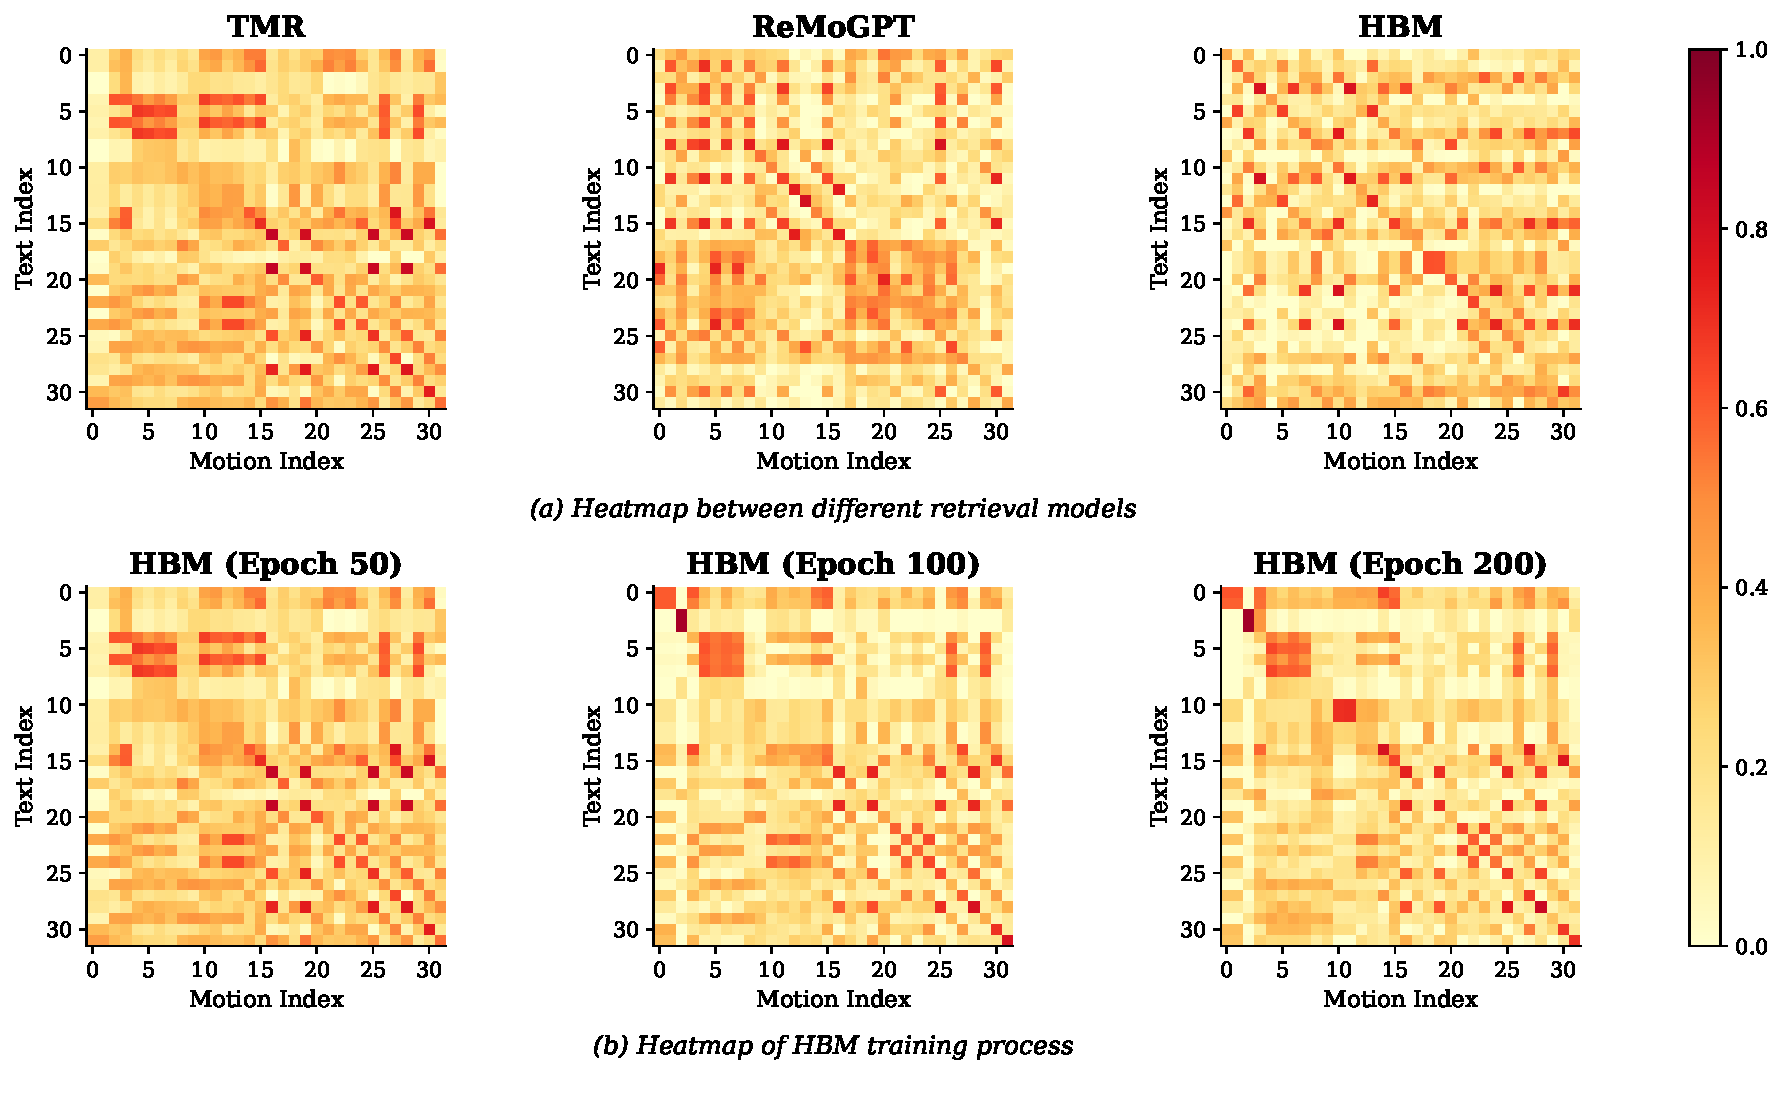
\includegraphics[width=\linewidth]{fig/heatmap.pdf}
        \caption{\textbf{Heatmap of similarity matrix.} The diagonal represents positive pairs, with darker colors meaning higher semantic similarity, conducted on HumanML3D.}
        \label{fig:heatmap}
\end{figure*}
\begin{figure*}[t!]
    \centering
    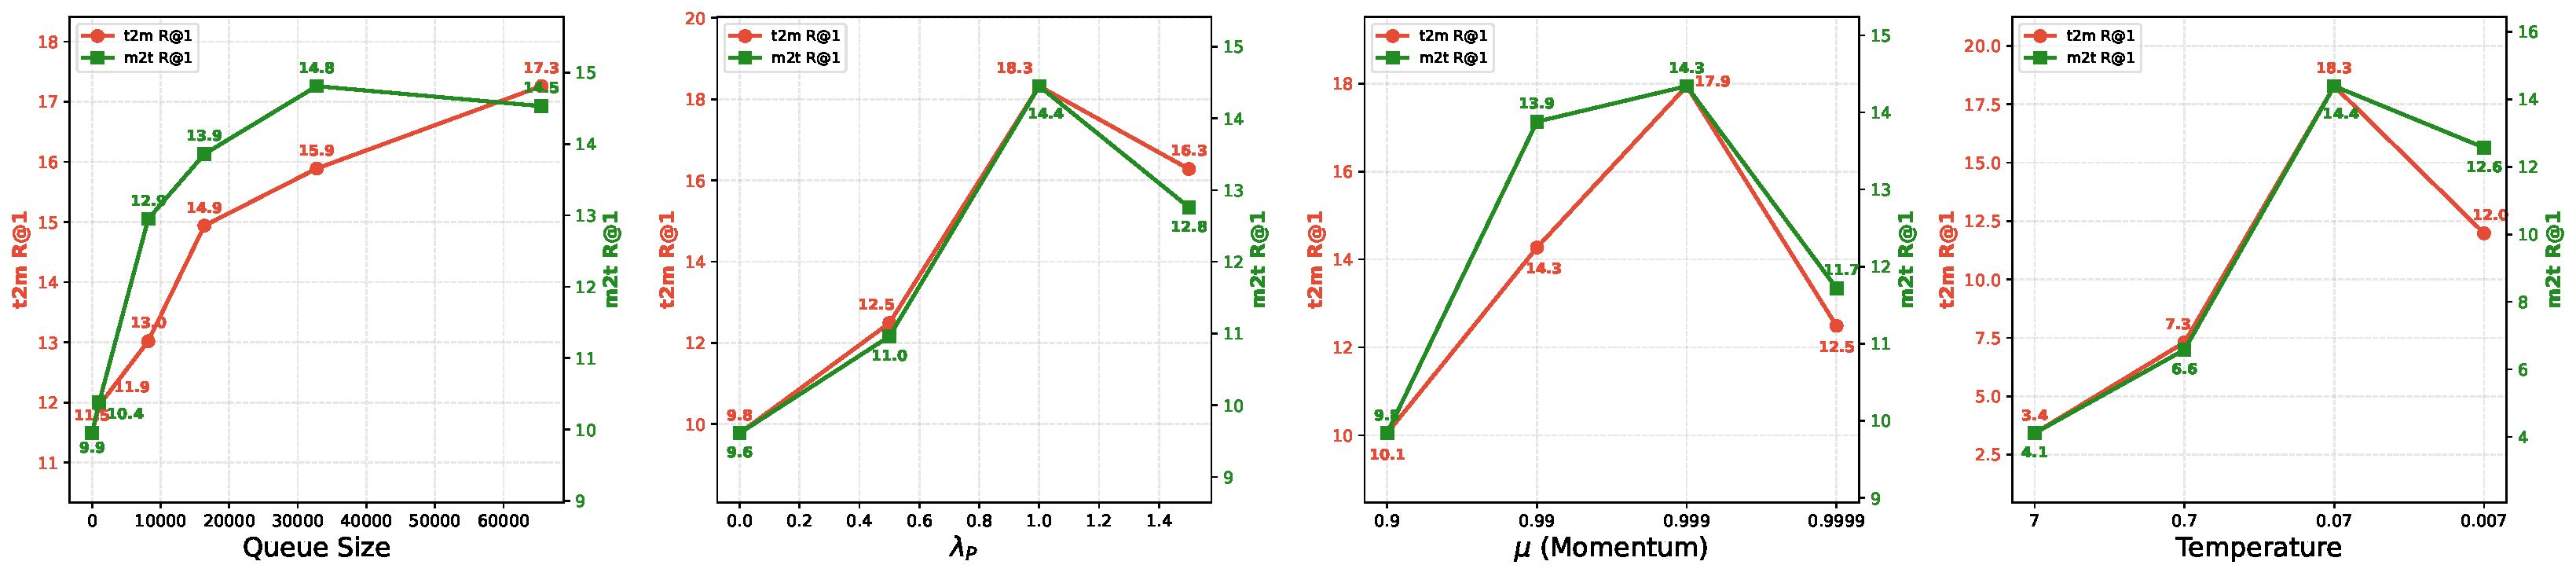
\includegraphics[width=\linewidth]{fig/hyperparameter.pdf}
        \caption{Sensitivity of contrastive training to key hyperparameters, conducted on HumanML3D.}
        \label{fig:hyperparameter}
\end{figure*}
% \begin{figure*}[t!]
%     \centering
%     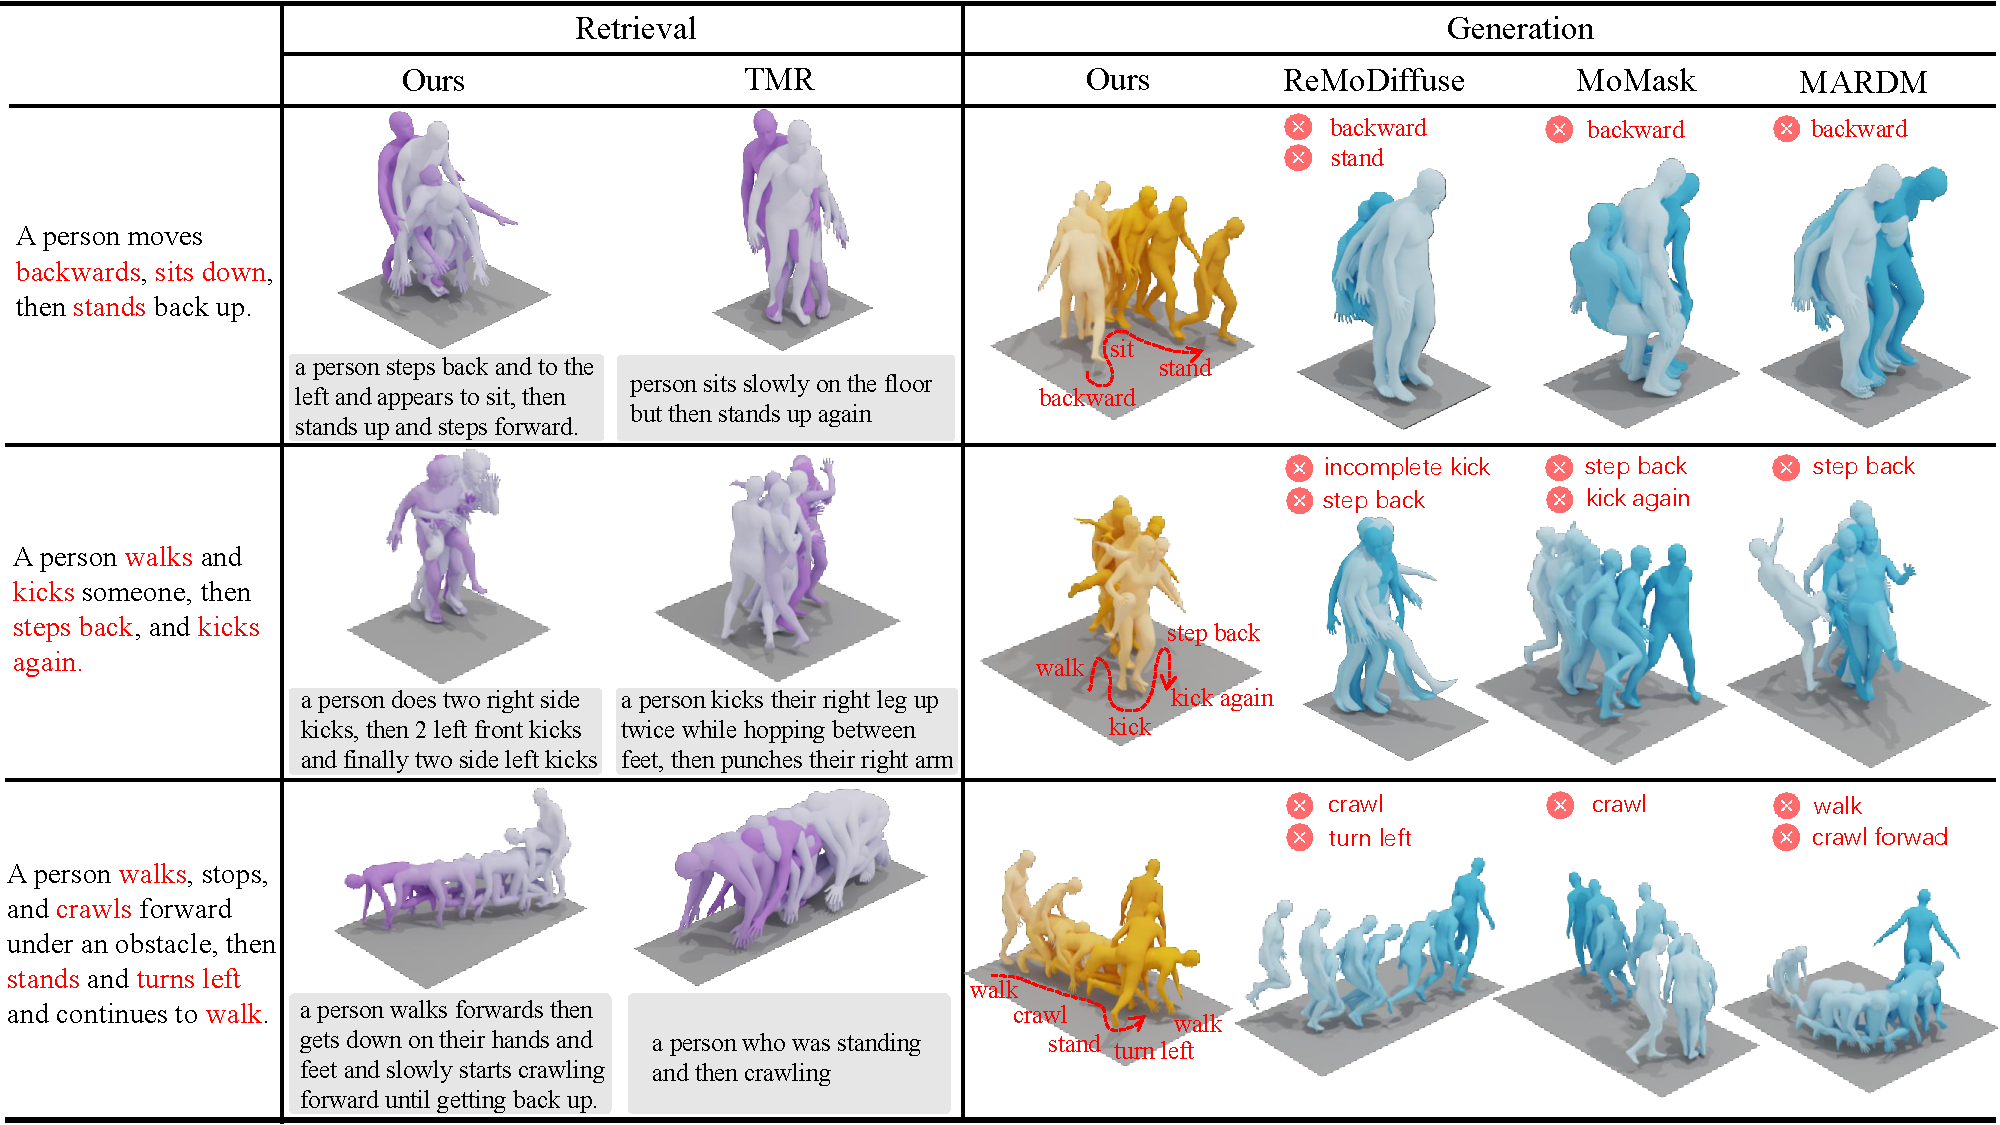
\includegraphics[width=\linewidth]{fig/rag_t2m_visual.pdf}
%         % \caption{\textbf{Heatmap of similarity matrix.} The diagonal represents positive pairs, with darker colors meaning higher semantic similarity, conducted on HumanML3D.}
%      \caption{\textbf{Qualitative comparisons.} The darker colors indicate the later in time. The motions generated by our method closely align with the descriptions, outperforming others that exhibit degraded motions or improper semantics.}
%     %     \label{fig:rag_t2m_visual}
% \end{figure*}




\subsection{Dataset and Evaluation Metrics}
We evaluate our model on HumanML3D~\cite{humanml3d}, KIT-ML~\cite{kitml}, and SnapMoGen~\cite{momask2} datasets. The HumanML3D consists of 14,616 motions and 44,970 texts, while KIT-ML consists of 3,911 motions and 6,278 texts. The SnapMoGen is the largest available dataset, comprising 20,450 motions and 122,565 texts. The motion feature dimensions are 263, 251, and 296 for HumanML3D, KIT-ML, and SnapMoGen, respectively. HumanML3D and KIT-ML are split into training, validation, and test sets with a ratio of \textbf{0.80:0.05:0.15}, while SnapMoGen uses a split of \textbf{0.85:0.05:0.10}.

\noindent \myparagraph{Evaluation Metrics.}
For text–motion retrieval, we report Recall at different ranks (R@1, R@2, R@3, R@5, and R@10), which measures the proportion of queries whose ground-truth match appears within the top-$k$ retrieved results. We also report the median rank (MedR), where lower values indicate better retrieval performance.
For motion generation, following prior work~\cite{momask,mogents}, we evaluate text-to-motion (T2M) performance from three perspectives: (1) motion quality, measured by the Frechet Inception Distance (FID); (2) generation diversity, evaluated using Diversity and Multi-Modality (MModality); and (3) text–motion alignment, assessed by R-Precision at top 1/2/3 and the Multi-Modal Distance (MM Dist). 
Formal definitions of each metric are provided below.

We report standard evaluation metrics widely adopted in text-to-motion generation following prior work~\cite{humanml3d}. All metrics are computed in a shared embedding space obtained from the pretrained evaluation networks introduced in~\cite{humanml3d}. We denote the feature representations of ground-truth motions, generated motions, and text descriptions as $f_{gt}$, $f_{pred}$, and $f_{text}$, respectively.

\paragraph{Frechet Inception Distance (FID).}
FID evaluates the distribution-level similarity between generated motions and ground-truth motions in the feature space. It is defined as

\begin{equation}
\begin{aligned}
\text{FID} = {} & \lVert \mu_{gt} - \mu_{pred} \rVert^2 \\
& + \mathrm{Tr}\!\left(
\Sigma_{gt} + \Sigma_{pred}
- 2(\Sigma_{gt}\Sigma_{pred})^{\frac{1}{2}}
\right)
\end{aligned}
\label{formula:fid}
\end{equation}

where $\mu_{gt}$ and $\mu_{pred}$ denote the empirical means of $f_{gt}$ and $f_{pred}$, and $\Sigma_{gt}$ and $\Sigma_{pred}$ are the corresponding covariance matrices.

\paragraph{R-Precision (Top-$k$).}
R-Precision assesses text--motion matching accuracy. For each generated motion, its ground-truth text description is combined with 31 randomly sampled mismatched descriptions from the test set to form a candidate pool. We rank all candidates according to the Euclidean distance between motion and text features, and report the retrieval accuracy at Top-1, Top-2, and Top-3. A retrieval is considered successful if the ground-truth description appears within the top-$k$ ranked results.

\paragraph{Multimodal Distance (MM-Dist).}
MM-Dist measures the alignment between generated motions and their corresponding text descriptions at the feature level. Given $N$ text--motion pairs, it is computed as the average Euclidean distance between motion and text features:
\begin{equation}
\text{MM-Dist} = \frac{1}{N}\sum_{i=1}^{N}\lVert f_{pred,i} - f_{text,i} \rVert .
\label{formula:mm-dis}
\end{equation}

\paragraph{Diversity.}
Diversity quantifies the overall variability of generated motions across the dataset. We randomly sample $S_{dis}$ pairs of generated motion features, denoted as $(f_{pred,i}, f'_{pred,i})$, and compute
\begin{equation}
\text{Diversity} = \frac{1}{S_{dis}}\sum_{i=1}^{S_{dis}} \lVert f_{pred,i} - f'_{pred,i} \rVert .
\label{formula:diversity}
\end{equation}
Following~\cite{humanml3d}, we set $S_{dis}=300$ in all experiments.

\paragraph{Multimodality (MModality).}
MModality evaluates the diversity of motions generated from the same text description. For each text input, we generate multiple motion samples and randomly select two subsets, each containing 10 motions. Let $(f_{pred,i,j}, f'_{pred,i,j})$ denote the feature pair from the $j$-th sample of the $i$-th text. MModality is computed as
\begin{equation}
\text{MModality} = \frac{1}{10N}\sum_{i=1}^{N}\sum_{j=1}^{10}\lVert f_{pred,i,j} - f'_{pred,i,j} \rVert .
\label{formula:mmodality}
\end{equation}

\subsection{Implementation Details}
For the motion representation, we use a pretrained 2D-RVQ-VAE~\cite{mogents} with 6 quantization layers, each containing a codebook of 512 codes of dimension 512.
% TODO-VERIFY (user decision needed): the actual checkpoint reports nb_code2d=256, code_dim2d=1024, which conflicts with the sentence above (ECCV text, kept verbatim). The new ReMoMask-2 paragraphs state d_e=1024 per the checkpoint. Reconcile before submission.
For the topology structured masking, we set $\pi_{base}$ to 0.5.
For the text–motion retrieval model, the motion encoder employs a 4-layer transformer for each body part, with both part-level and instance-level motion embeddings set to 512 dimensions. 
The text encoder is a frozen pretrained CLIP~\cite{clip} ViT-B/32 model with one additional trainable transformer layer, shared across all models. 
For the motion masked model, the SSTA is set to have 6 layers, 8 heads, and 512 latent dimensions. The retrieval model is trained for 200 epochs on a Tesla A800 GPU, with a $\lambda_{P}$ of 1, a batch size of 128, a queue size of 65,536, and a momentum $\mu$ of 0.999.
The masked models are trained on 8 Tesla A800 GPUs for up to 2,000 epochs with a batch size of 64. All models are implemented in PyTorch.

\noindent \myparagraph{ReMoMask-2.}
The $z_e$ retrieval database is constructed once from the frozen 2D-RVQ-VAE: each of the 23,384 training motions is passed through the 2D encoder, and its pre-quantization latent (1024 channels over the temporal--part grid) is mean-pooled over the temporal and part axes and $\ell_2$-normalized to form a 1024-dimensional retrieval key; expanding motions to their captions yields 66,912 (motion, caption) entries, and the full build takes about five minutes. The query projector $\phi$ is a two-layer MLP (Linear $512{\to}1024$, GELU, Linear $1024{\to}1024$; $\approx$1.57M parameters) applied to the frozen CLIP~\cite{clip} ViT-B/32 text embedding already used to condition the masked generator, with $\ell_2$-normalized outputs. It is trained for 200 epochs with a batch size of 128 on a single GPU using Adam with cosine annealing, distilling the HBM retriever's top-256 soft targets at temperature $\tau = 0.07$; the VQ-VAE remains frozen throughout. On the generator side, the SSTA architecture is unchanged: the only additional parameters are two linear adapters ($1024 \to 512$) that project the retrieved $R_m$ and $R_t$ to the model dimension. For the controlled comparison in this journal version, the masked models of ReMoMask and ReMoMask-2 are trained under exactly the same configuration---identical backbone, optimization hyper-parameters, batch size, training schedule, and random seed, with the value-pathway routing of Section~\ref{subsec:vroute} enabled in both variants---so that the retrieval space is the only varying factor between the two systems.



\subsection{Main Results}
\noindent \myparagraph{Evaluation of Motion Retrieval.}
We evaluate ReMoMask on text-motion and motion-text retrieval on HumanML3D, KIT-ML, and SnapMoGen (Table~\ref{tab:rag_experiment}), achieving state-of-the-art performance across all benchmarks.
ReMoMask consistently outperforms prior methods on HumanML3D and SnapMoGen, improving text-to-motion R@1 on HumanML3D by 68.09\% over ReMoGPT (18.49 vs.~11.00) and increasing R@1 on SnapMoGen from 8.92 to 12.43. On KIT-ML, ReMoMask achieves the best performance at higher recall levels (R@5 and R@10), indicating robust retrieval.
Fig.~\ref{fig:heatmap} further shows that HBM yields clearer diagonal structures with suppressed off-diagonal responses, confirming more accurate and discriminative text–motion alignment.
For ReMoMask-2, the same benchmarks probe the ranking quality of the distilled projector $\phi$ in the $z_e$ space (ReMoMask-2 rows in Table~\ref{tab:rag_experiment}); \textbf{[TBD: one-sentence comparison against HBM once numbers land]}.

\noindent \myparagraph{Evaluation of Motion Generation.}
We evaluate motion generation performance on the HumanML3D, KIT-ML, and SnapMoGen datasets, as illustrated in Table~\ref{tab:t2m_experiment}. ReMoMask consistently achieves strong motion generation performance, as reflected by consistently lower FID scores compared to prior state-of-the-art methods across all three benchmarks. On KIT-ML and SnapMoGen, some baselines achieve slightly higher Diversity or MModality, which is expected for retrieval-augmented generation methods that prioritize semantic alignment and motion coherence.
ReMoMask-2 further improves over ReMoMask on all three benchmarks (\textbf{[TBD]}), with the controlled protocol of Section~\ref{subsec:ablation_v2} attributing the gain to the retrieval space.

\noindent \myparagraph{Qualitative comparisons.}
We compare our method with others in Fig.~\ref{fig:rag_t2m_visual}. The visualizations demonstrate that our model achieves superior motion realism and better text-motion alignment.




%% --- Additional Comparisons (from extended analysis) ---

\textbf{Inference Efficiency Comparison.}
Beyond generation quality, we compare our method with existing approaches in terms of both FID and inference cost. As shown in Fig.~\ref{fig:scatter}, ReMoMask achieves a favorable trade-off between generation quality and computational efficiency compared to other retrieval-augmented and non-retrieval methods.

\begin{figure}[t]
    \centering
% 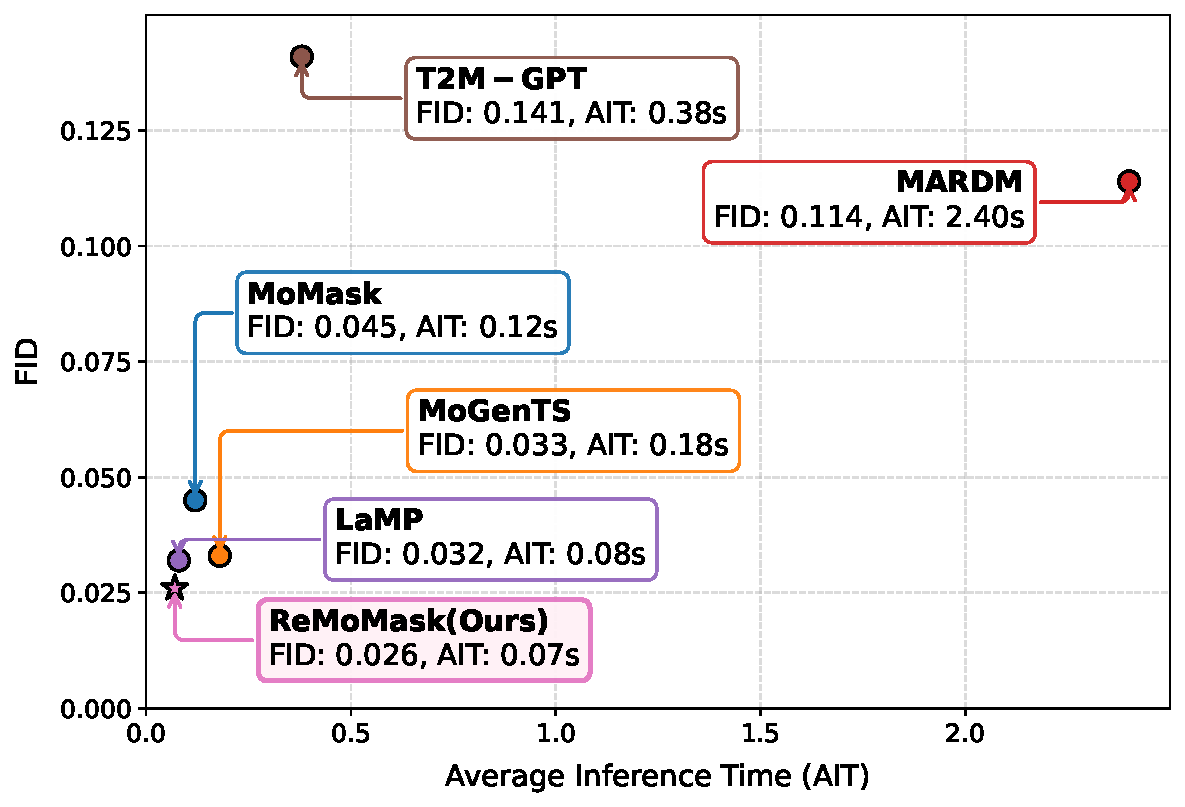
\includegraphics[width=\linewidth]{fig/scatter_rebuttal.pdf}
    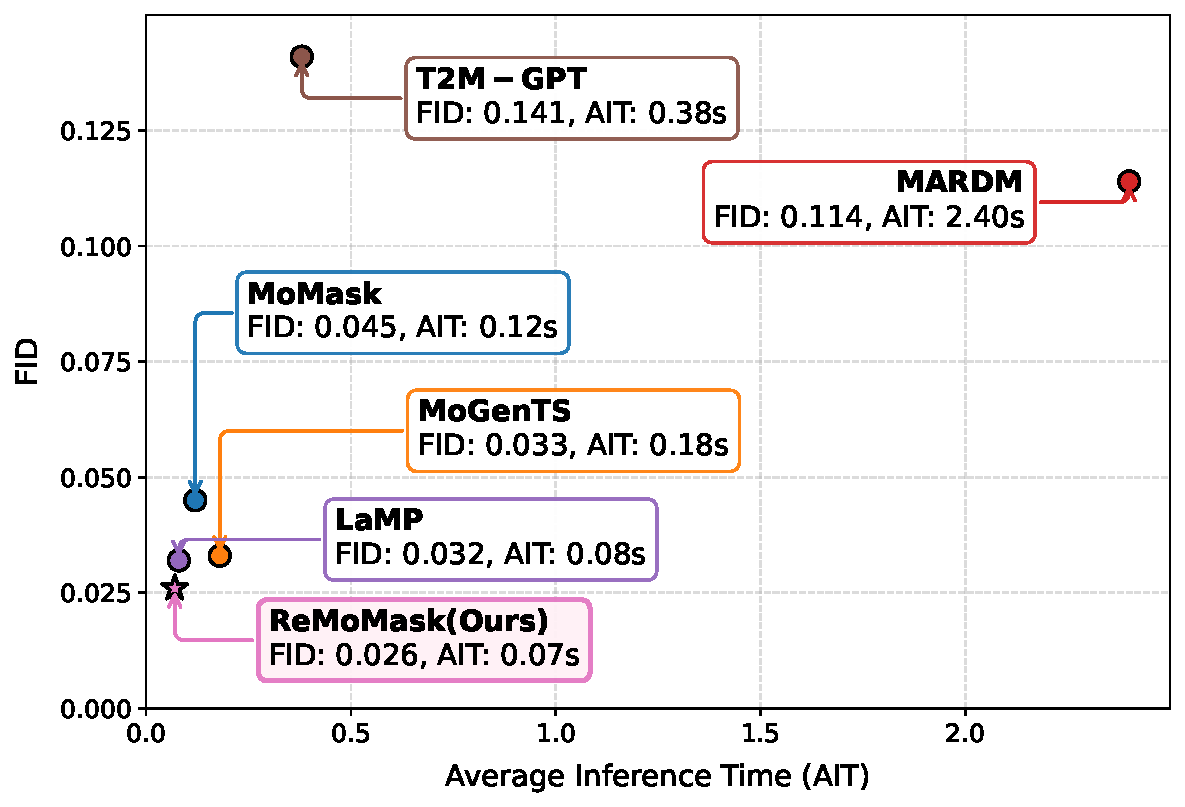
\includegraphics[width=0.80\linewidth]{fig/scatter_rebuttal.pdf}
    \vspace{-10pt}
    \caption{Comparison on FID and Inference Cost.}
    \vspace{-10pt}
    \label{fig:scatter}
\end{figure}

\textbf{Generalization Across Backbones.}
To validate the generalizability of our HBM module, we integrate it with different backbone architectures. As shown in Table~\ref{tab:cross}, HBM consistently improves performance across backbones, reducing FID while maintaining or improving other metrics, demonstrating its effectiveness as a general-purpose retrieval-augmented component.

\begin{table}[t]
    \centering
    % \small
    \caption{Generalization across backbones on HumanML3D.}
    \label{tab:cross}
    \renewcommand{\arraystretch}{1.0}  % Adjust the line height (global)
    \resizebox{0.8\linewidth}{!}{
    \begin{tabular}{cc|cccc}
        \toprule
        BaseModel & Encoder & FID$\downarrow$ & Top1$\uparrow$ & Top2$\uparrow$ & Top3$\uparrow$ \\
        \hline
        \hline
        \multirow{2}{*}{ReMoDiffuse} & Clip & 0.103 & 0.510 & 0.698 & 0.795 \\
         & HBM & 0.091({\color{mygreen}-0.012}) & 0.515 & 0.708 & 0.799 \\
         \hline
        \multirow{2}{*}{ReMoGPT} & Transformer & 0.205 & 0.501 & 0.688 & 0.792 \\
         & HBM & 0.165({\color{mygreen}-0.040}) & 0.505 & 0.693 & 0.794 \\
        \bottomrule
    \end{tabular}
    }
\end{table}

\subsection{Ablation Study}
We conduct ablation studies on the HumanML3D dataset to investigate the impact of motion latent representations, fusion strategies, mask strategy, and retriever designs. Quantitative results reported in Table~\ref{tab:ablation_ssta} show that all the proposed components contribute greatly.


            



% \myparagraph{Latent Representation and Fusion.} Replacing the 1D motion latent with a 2D latent improves performance, reducing FID from $0.132$ to $0.121$ and increasing Top-1 R-Precision from $0.498$ to $0.515$. Substituting SSTA with concatenation degrades performance, increasing FID from $0.097$ to $0.116$ and reducing Top-1 R-Precision from $0.528$ to $0.493$. These results demonstrate the benefit of richer spatial-temporal representations and a tailored fusion mechanism.

% \myparagraph{Retriever Design.} Replacing InfoNCE with HBM yields a substantial improvement, reducing FID from $0.121$ to $0.097$ and improving Top-1 R-Precision from $0.515$ to $0.528$. Therefore HBM contributes greatly to ReMoMask.

\noindent \myparagraph{Hierarchical Level.}
Table~\ref{tab:ablation_hierarchical} compares single-level and hierarchical retrieval under identical settings, showing that combining instance-level and part-level supervision consistently yields the best retrieval performance. While instance-level alignment captures coarse semantics and part-level alignment alone is insufficient, their hierarchical combination provides complementary information across abstraction levels, enabling more accurate and robust text–motion alignment.



\noindent \myparagraph{Momentum Encoder.}
We evaluate the effect of momentum encoders in contrastive retrieval training in Table~\ref{tab:ablation_momentum_encoder}. Introducing momentum encoders consistently improves both text-to-motion and motion-to-text retrieval.

\noindent \myparagraph{Information Source.}
We investigate the roles of different information sources within the SSTA key and value matrices on the HumanML3D dataset. Under identical settings (Table~\ref{tab:ablation}), our results reveal a clear functional asymmetry: enriching the key matrix with retrieved information consistently improves performance, indicating that the key primarily acts as a selector that benefits from diverse reference signals. However, constraining the value matrix leads to better results, as injecting excessive or misaligned information into values can degrade generation quality, suggesting that effective SSTA design requires rich keys for attention selection and controlled values for stable information aggregation.




\begin{table}[t]
% \begin{table}[t]  
    \centering
    \caption{The impacts of different information source selections for key and value matrices in SSTA on t2m task, conducted on the HumanML3D dataset.}
    \label{tab:ablation}
    % \begin{minipage}[t]{0.48\textwidth}
    \renewcommand{\arraystretch}{1.3}  % Adjust the line height (global)
    \resizebox{\columnwidth}{!}{
        \begin{tabular}{ccc|ccc|c|c|c}
            \toprule
            \multicolumn{3}{c|}{K Matrix} & \multicolumn{3}{c|}{V Matrix} & \multirow{2}{*}{FID$\downarrow$} & \multicolumn{1}{c|}{R-Precision$\uparrow$} & \multirow{2}{*}{MMDIST$\downarrow$}  \\
            \cline{1-6}
            \cline{8-8}
            $t$ & $R_t$ & $R_m$ & $t$ & $R_t$ & $R_m$ & & Top1 & \\
            \hline
            \hline
            $\checkmark$ & $\checkmark$ & $\checkmark$  & $\checkmark$  & $\checkmark$  & $\checkmark$  & \underline{$0.043^{\pm{.007}}$} & \underline{$0.548^{\pm{.008}}$} & $2.896^{\pm{.007}}$ \\
            $\checkmark$ & $\checkmark$ & $\checkmark$  &  & $\checkmark$  & $\checkmark$  &$0.104^{\pm{.005}}$ &$0.506^{\pm{.004}}$ & $\mathbf{2.865^{\pm{.005}}}$\\
            \rowcolor[gray]{0.90}  $\checkmark$ & $\checkmark$ & $\checkmark$  & & & $\checkmark$  & $\mathbf{0.027^{\pm{.005}}}$ & $\mathbf{0.562^{\pm{.004}}}$ & $2.877^{\pm{.008}}$ \\
            $\checkmark$ & & $\checkmark$  &  &  & $\checkmark$  & $0.073^{\pm{.003}}$ & $0.536^{\pm{.003}}$ & $\underline{2.872^{\pm{.005}}}$\\
            $\checkmark$ & $\checkmark$ &   &  & & $\checkmark$  & $0.096^{\pm{.007}}$ & $0.513^{\pm{.005}}$ & $2.973^{\pm{.005}}$\\
            $\checkmark$ &  &   &  & & $\checkmark$  &$0.194^{\pm{.005}}$ & $0.476^{\pm{.012}}$ & $3.242^{\pm{.013}}$\\
            \bottomrule
        \end{tabular}
    }
    % \end{minipage}
% \end{table}
\end{table}



\noindent \myparagraph{Hyperparameters.}
We analyze the sensitivity of HBM contrastive training to key hyperparameters on HumanML3D in Fig.~\ref{fig:hyperparameter}. Larger queue sizes improve retrieval by providing more negatives, while optimal performance is achieved with moderate values of $\lambda_P$, temperature, and momentum, indicating a balanced and stable training regime.

\noindent \myparagraph{Database Coverage.}
We further analyze the impact of database coverage on retrieval-augmented motion generation. 
Specifically, we vary the percentage of the training database accessible during retrieval and evaluate both semantic alignment (R-Precision Top1) and generation quality (FID) on HumanML3D. As shown in Fig.~\ref{fig:db_coverage}, increasing database coverage from 10\% to 100\% reduces FID by 64\% (0.073→0.026) while improving R-Precision from 0.502 to 0.566, demonstrating that richer retrieval databases substantially enhance generation quality.

\noindent \myparagraph{Efficiency}
Following \cite{momask}, we evaluate the efficiency and quality of motion generation using various methods. The inference cost is quantified as the mean inference time over 100 samples on a single Nvidia 2080Ti device. As shown in Fig.~\ref{fig:scatter}, ReMoMask offers better quality-efficiency trade-offs than baseline methods.



\begin{figure}[t]
     \centering
     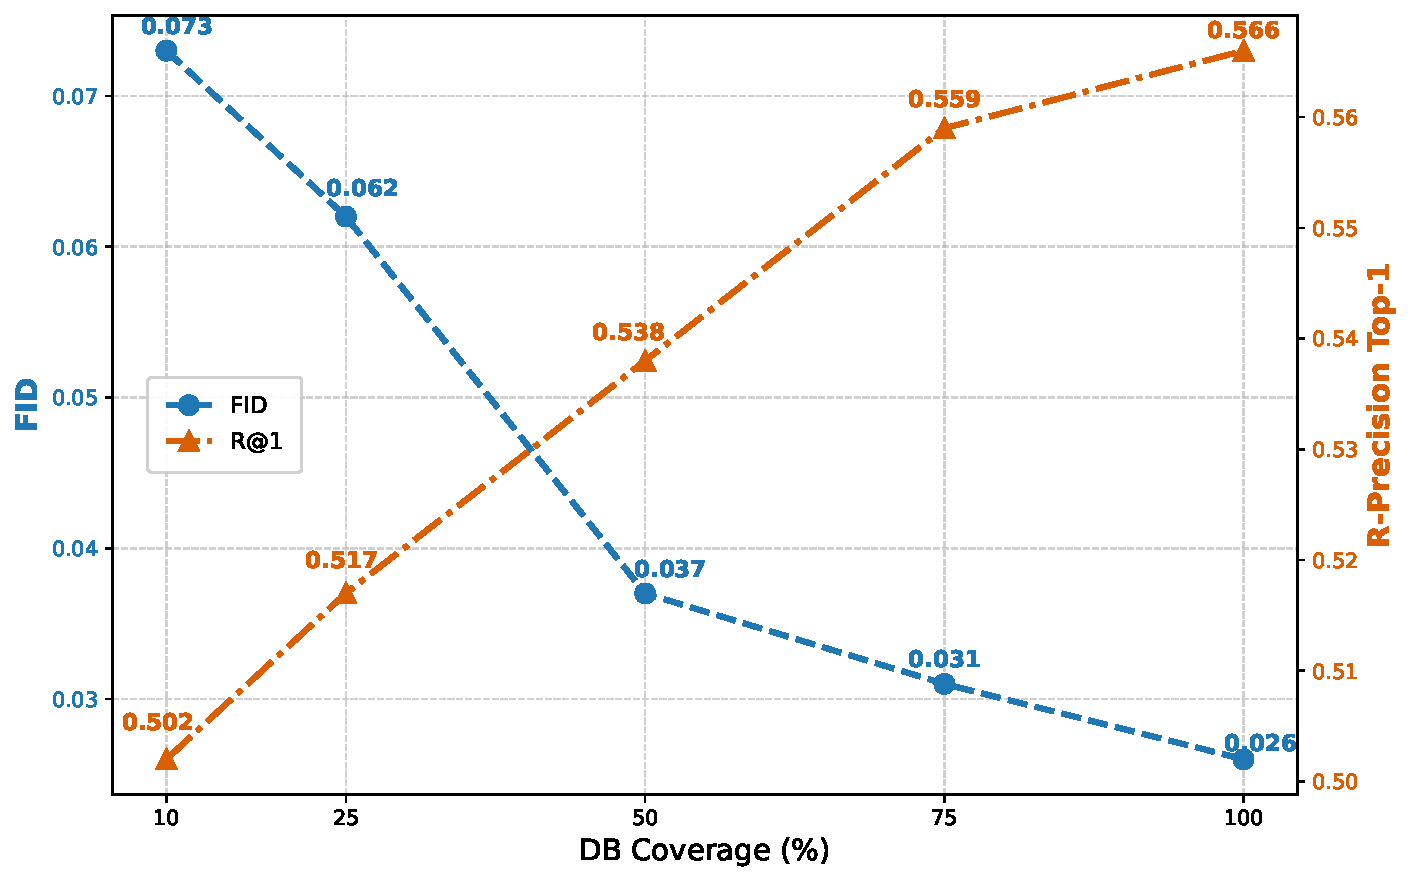
\includegraphics[width=0.85\linewidth]{fig/db_coverage.pdf}
     \caption{\textbf{Impact of database coverage.} A richer retrieval database substantially enhances generation quality.}
     \label{fig:db_coverage}
     
\end{figure}






%% --- Additional Ablation Studies (from extended analysis) ---

\textbf{Masking Strategy Comparison.}
We compare our topology structured masking (TSM) with the commonly used cosine scheduling strategy on HumanML3D. As shown in Table~\ref{fig:mask}, TSM achieves a lower FID (0.025) compared to cosine scheduler masking (0.034), while maintaining comparable diversity and multimodality, demonstrating the effectiveness of our structure-aware masking approach.

\begin{table}[t]
    \centering
    % \small
    \caption{Comparison of masking strategies on HumanML3D.}
    \label{fig:mask}
    \renewcommand{\arraystretch}{1.0}  % Adjust the line height (global)
    \resizebox{1.0\linewidth}{!}{
    \begin{tabular}{l|cccc}
        \toprule
        Masking strategies & FID$\downarrow$ & Top1$\uparrow$ & Top2$\uparrow$ & Top3$\uparrow$ \\
        \hline
        \hline
        cosine scheduler masking & 0.034 & 0.556 & 0.751 & 0.842 \\
        topology structured masking & 0.025({\color{mygreen}-0.009}) & 0.567 & 0.764 & 0.848 \\
        \bottomrule
    \end{tabular}
    }
\end{table}

\textbf{Retrieval Fusion Design.}
We investigate how different fusion strategies affect the integration of retrieved motion information. Table~\ref{tab:fusion} compares concatenation, cross-attention, and adaptive fusion approaches, examining their impact on generation quality when combined with different retrieval representations.

\begin{table}[t]
    \centering
    % \small
    \renewcommand{\arraystretch}{1.0}  % Adjust the line height (global)
    % \setlength{\tabcolsep}{4pt}  % Adjust the column margin
    \caption{Comparison of retrieval fusion design on HumanML3D.}
    \label{tab:fusion}
    \resizebox{1.\linewidth}{!}{
        \begin{tabular}{c|cccc|cccc}
            \toprule
                \multirow{2}{*}{Fusion} &  \multicolumn{4}{c|}{Text-motion retrieval} & \multicolumn{4}{c}{Motion-text retrieval} \\
                \cline{2-9}
                & R@1 $\uparrow$ & R@5 $\uparrow$ & R@10 $\uparrow$  & MedR $\downarrow$ & R@1 $\uparrow$ & R@5 $\uparrow$ & R@10 $\uparrow$ & MedR $\downarrow$ \\
            \hline
            \hline
                Max-Pooling  & 1.22 & 6.57 & 10.83 & 198.00 & 1.45 & 7.69 & 12.75 & 173.50 \\
                Mean-Pooling & 6.54 & 22.11 & 31.74 & 28.50 & 4.90 & 19.15 & 28.36 & 32.00 \\
                MLP & 18.39 & 32.25 & 45.37 & 11.50 & 14.35 & 31.62 & 45.46 & 17.00 \\ 
            \bottomrule
        \end{tabular}
    }
\end{table}

\textbf{Temporal Retrieval Analysis.}
We evaluate the impact of incorporating temporal information in the retrieval component. Table~\ref{tab:temporal} shows that considering temporal alignment during retrieval, as measured by the CAR metric~\cite{CAR}, further improves generation quality on HumanML3D.

\begin{table}[t]
    \centering
    % \small
    \renewcommand{\arraystretch}{1.0}  % Adjust the line height (global)
    % \setlength{\tabcolsep}{4pt}  % Adjust the column margin
    \caption{Temporal retrieval experiment on HumanML3D.}
    \label{tab:temporal}
    \resizebox{1.\linewidth}{!}{
        \begin{tabular}{c|cccc|cccc}
            \toprule
                \multirow{2}{*}{Method} &  \multicolumn{4}{c|}{Text-motion retrieval} & \multicolumn{4}{c}{Motion-text retrieval} \\
                \cline{2-9}
                & R@1$\uparrow$ & R@5$\uparrow$ & R@10$\uparrow$ & CAR$\uparrow$ & R@1$\uparrow$ & R@5$\uparrow$  & R@10$\uparrow$ & CAR$\uparrow$ \\
            \hline
            \hline
                TMR  & 5.96 & 20.61 & 30.74 & 63.24 & 9.97 & 23.22 & 32.35 & 64.83 \\
                ReMoGPT  & 11.02 & 29.98 & 43.04 & 68.50 & 12.81 & 28.43 & 39.58 & 67.09 \\
                HBM  & 18.43 & 32.60 & 46.34 & 77.29 & 14.98 & 30.86 & 44.82 & 75.06 \\
            \bottomrule
        \end{tabular}
    }
\end{table}

\textbf{Complete Retrieval Ablation.}
Table~\ref{tab:rag_ablation} provides a comprehensive ablation study of the retrieval components, analyzing the individual and combined contributions of hierarchical text-motion alignment and the HBM module across different backbone architectures.

\begin{table}[t]
    \centering
    % \small
    \renewcommand{\arraystretch}{1.0}  % Adjust the line height (global)
    % \setlength{\tabcolsep}{4pt}  % Adjust the column margin
    \caption{Complete retrieval ablation analysis on HumanML3D.}
    \label{tab:rag_ablation}
    \resizebox{1.\linewidth}{!}{
        \begin{tabular}{c|cc|ccc|ccc}
            \toprule
                \multirow{2}{*}{Momentum} & \multicolumn{2}{c|}{Hierarchical Level}&  \multicolumn{3}{c|}{Text-motion retrieval} & \multicolumn{3}{c}{Motion-text retrieval} \\
                \cline{2-9}
                & Part & Instance & R@1 $\uparrow$ & R@5 $\uparrow$ & MedR $\downarrow$ & R@1 $\uparrow$ & R@5 $\uparrow$ & MedR $\downarrow$ \\
            \hline
            \hline
                $\times$  & $\checkmark$  & $\times$  & 7.32 & 21.25 & 27.00 & 7.95 & 23.68  & 28.00 \\
                $\times$  & $\times$ & $\checkmark$   & 11.50 & 28.45 & 18.00 & 11.41 & 27.19  & 19.00 \\ 
                $\times$  & $\checkmark$  & $\checkmark$   & 14.87 & 30.65 & 16.00 & 13.78 & 28.68  & 18.50 \\
                $\checkmark$  & $\checkmark$ & $\times$  & 7.98 & 21.44 & 26.00 & 8.12 & 23.26  & 27.50 \\
                $\checkmark$  & $\times$ & $\checkmark$  & 12.67 & 30.95 & 16.00 & 13.27 & 29.46  & 17.50 \\ 
                $\checkmark$  & $\checkmark$ & $\checkmark$  & 18.34 & 32.62 & 12.50 & 14.59 & 30.58  & 16.00 \\
            \bottomrule
        \end{tabular}
    }
\end{table}


%============================================================
% V2 (journal version) ablations
%============================================================
\subsection{Ablation Study of ReMoMask-2}
\label{subsec:ablation_v2}
The ablations above isolate the contributions of HBM, TSM, and SSTA. We now ablate the two additions of the journal version: the latent-aligned retrieval space (Section~\ref{subsec:lar}) and the re-enabled value-pathway routing (Section~\ref{subsec:vroute}).
Unless stated otherwise, all variants share the identical backbone, masking strategy, and training configuration, and are evaluated on HumanML3D with the full generation pipeline under the same protocol as Table~\ref{tab:t2m_experiment}.

\begin{table}[t]
    \centering
    \caption{\textbf{Orthogonal ablation of retrieval space and value-pathway routing on HumanML3D.} All four variants share the identical backbone, masking strategy, and training configuration; only the retrieval space (semantic HBM space vs.\ latent-aligned $z_e$ space) and the routing of the retrieved text embedding $R_t$ into the Value pathway vary. The first row corresponds to the conference ReMoMask configuration retrained under the journal protocol; the last row is the full ReMoMask-2.}
    \label{tab:ablation_v2_orthogonal}
    \renewcommand{\arraystretch}{1.3}  % Adjust the line height (global)
    \resizebox{\columnwidth}{!}{
        \begin{tabular}{l| c| c| c| c}
            \toprule
            Retrieval Space & $R_t$ in Value & FID$\downarrow$ & Top1$\uparrow$ & MMDIST$\downarrow$ \\
            \hline
            \hline
            Semantic (HBM) & $\times$ & $x.xxx^{\pm.xxx}$ & $x.xxx^{\pm.xxx}$ & $x.xxx^{\pm.xxx}$ \\
            Semantic (HBM) & $\checkmark$ & $x.xxx^{\pm.xxx}$ & $x.xxx^{\pm.xxx}$ & $x.xxx^{\pm.xxx}$ \\
            Latent-aligned ($z_e$) & $\times$ & $x.xxx^{\pm.xxx}$ & $x.xxx^{\pm.xxx}$ & $x.xxx^{\pm.xxx}$ \\
            \rowcolor{yellow!20} Latent-aligned ($z_e$) & $\checkmark$ & $x.xxx^{\pm.xxx}$ & $x.xxx^{\pm.xxx}$ & $x.xxx^{\pm.xxx}$ \\
            \bottomrule
        \end{tabular}
    }
\end{table}

\begin{table}[t]
    \centering
    \caption{Alignment objective for the query projector $\phi$ on HumanML3D. Retrieval columns report text-to-motion recall of the projected query in the $z_e$ space; FID reports downstream generation quality when the resulting projector is used in ReMoMask-2. The adopted setting is shaded.}
    \label{tab:ablation_v2_alignment}
    \renewcommand{\arraystretch}{1.3}  % Adjust the line height (global)
    \resizebox{\columnwidth}{!}{
        \begin{tabular}{l| ccc| c}
            \toprule
            Objective & R@1$\uparrow$ & R@5$\uparrow$ & R@10$\uparrow$ & FID$\downarrow$ \\
            \hline
            \hline
            InfoNCE & xx.xx & xx.xx & xx.xx & $x.xxx^{\pm.xxx}$ \\
            \rowcolor[gray]{0.90} KL distillation & xx.xx & xx.xx & xx.xx & $x.xxx^{\pm.xxx}$ \\
            \bottomrule
        \end{tabular}
    }
\end{table}

\begin{table}[t]
    \centering
    \caption{Choice of the distillation teacher for the query projector $\phi$ on HumanML3D. The projector is distilled from each teacher's top-256 soft targets under otherwise identical settings. The adopted setting is shaded.}
    \label{tab:ablation_v2_teacher}
    \renewcommand{\arraystretch}{1.3}  % Adjust the line height (global)
    \resizebox{\columnwidth}{!}{
        \begin{tabular}{l| ccc| c}
            \toprule
            Teacher & R@1$\uparrow$ & R@5$\uparrow$ & R@10$\uparrow$ & FID$\downarrow$ \\
            \hline
            \hline
            TMR~\cite{tmr} & xx.xx & xx.xx & xx.xx & $x.xxx^{\pm.xxx}$ \\
            \rowcolor[gray]{0.90} HBM & xx.xx & xx.xx & xx.xx & $x.xxx^{\pm.xxx}$ \\
            \bottomrule
        \end{tabular}
    }
\end{table}

\begin{table}[t]
    \centering
    \caption{Sensitivity of the query projector to the number of distillation targets (top-$\kappa$) and to projector capacity, measured by text-to-motion recall on HumanML3D. Default settings are shaded.}
    \label{tab:ablation_v2_sensitivity}
    \renewcommand{\arraystretch}{1.3}  % Adjust the line height (global)
    \resizebox{\columnwidth}{!}{
        \begin{tabular}{l| c| ccc}
            \toprule
             & \#Params & R@1$\uparrow$ & R@5$\uparrow$ & R@10$\uparrow$ \\
            \hline
            \hline
            \multicolumn{5}{l}{\emph{Distillation top-$\kappa$}} \\
            \hline
            $\kappa{=}64$ & 1.57M & xx.xx & xx.xx & xx.xx \\
            \rowcolor[gray]{0.90} $\kappa{=}256$ (default) & 1.57M & xx.xx & xx.xx & xx.xx \\
            $\kappa{=}1024$ & 1.57M & xx.xx & xx.xx & xx.xx \\
            \hline
            \multicolumn{5}{l}{\emph{Projector capacity}} \\
            \hline
            Linear ($512{\to}1024$) & 0.53M & xx.xx & xx.xx & xx.xx \\
            \rowcolor[gray]{0.90} MLP, hidden 1024 (default) & 1.57M & xx.xx & xx.xx & xx.xx \\
            MLP, hidden 2048 & 3.15M & xx.xx & xx.xx & xx.xx \\
            \bottomrule
        \end{tabular}
    }
\end{table}

\begin{table}[t]
    \centering
    \caption{Mask-Transformer-only diagnosis on HumanML3D. Each system is evaluated with the Mask Transformer alone (no residual refinement) and with the full generation pipeline, under otherwise identical settings and the controlled training protocol of this journal version.}
    \label{tab:ablation_v2_maskonly}
    \renewcommand{\arraystretch}{1.3}  % Adjust the line height (global)
    \resizebox{\columnwidth}{!}{
        \begin{tabular}{l| cc| cc}
            \toprule
            \multirow{2}{*}{Method} & \multicolumn{2}{c|}{Mask Transformer only} & \multicolumn{2}{c}{Full pipeline} \\
            \cline{2-5}
            & FID$\downarrow$ & Top1$\uparrow$ & FID$\downarrow$ & Top1$\uparrow$ \\
            \hline
            \hline
            ReMoMask & $x.xxx^{\pm.xxx}$ & $x.xxx^{\pm.xxx}$ & $x.xxx^{\pm.xxx}$ & $x.xxx^{\pm.xxx}$ \\
            \rowcolor{yellow!20} \textbf{ReMoMask-2} & $x.xxx^{\pm.xxx}$ & $x.xxx^{\pm.xxx}$ & $x.xxx^{\pm.xxx}$ & $x.xxx^{\pm.xxx}$ \\
            \bottomrule
        \end{tabular}
    }
\end{table}

\noindent \myparagraph{Retrieval Space and Value Routing.}
Table~\ref{tab:ablation_v2_orthogonal} disentangles the two journal-version factors. The retrieval space is the dominant one: switching from the semantic HBM space to the latent-aligned $z_e$ space reduces FID by \textbf{[TBD]} without routing and by \textbf{[TBD]} with routing, together with consistent gains in Top-1 R-Precision. Routing $R_t$ into the Value pathway contributes a smaller gain in both retrieval spaces (\textbf{[TBD]} and \textbf{[TBD]} FID reduction, respectively), and the two effects compose nearly additively: the full configuration ($z_e$ + routing) attains the best results across all three metrics, indicating that the two contributions are largely independent.

The routing result should be read against the premise it rests on. In the conference version, $R_t$ was a text-domain signal from the contrastive semantic space, and injecting it into the Value pathway degraded quality (FID $0.104$ vs.\ $0.027$ in Table~\ref{tab:ablation}), which motivated excluding textual semantics from Value to prevent domain mismatch. In ReMoMask-2, $R_t$ is projected by $\phi$ into the motion-aligned $z_e$ space and thus enters SSTA as a motion-domain signal; the premise behind the exclusion no longer applies to it, and re-enabling the routing is accordingly beneficial, with the clearly larger gain observed in the latent-aligned rows (\textbf{[TBD]}). The modest positive effect in the semantic-space rows (\textbf{[TBD]}) suggests that the routing penalty observed at the conference operating point does not carry over unchanged to the journal re-evaluation; it does not overturn the conference finding, which isolates a semantic-space $R_t$ under the original protocol.

\noindent \myparagraph{Where the Gain Arises: Mask-Transformer-Only Diagnosis.}
The full pipeline refines the Mask Transformer's output with a residual stage, which could in principle either absorb or amplify differences between retrieval spaces. Table~\ref{tab:ablation_v2_maskonly} therefore evaluates both systems with the residual stage removed. The latent-aligned advantage is already present at the mask-only stage (\textbf{[TBD]} FID reduction over ReMoMask) and persists at a comparable relative magnitude through residual refinement (\textbf{[TBD]}), indicating that better-aligned retrieval evidence improves the coarse token prediction itself rather than relying on downstream refinement to compensate for cross-space noise.

\noindent \myparagraph{Alignment Objective.}
Table~\ref{tab:ablation_v2_alignment} compares KL distillation with InfoNCE for training $\phi$. KL distillation yields both higher projector recall and lower downstream FID (\textbf{[TBD]}). This is consistent with the distillation view of the alignment problem: the projector does not need to learn a text--motion metric from scratch, but to reproduce, inside the $z_e$ space, the ranking of an existing stronger retriever. The top-256 soft targets convey the teacher's full similarity structure over candidates, whereas InfoNCE reduces supervision to a single positive per caption; since the database expands 23,384 motions into 66,912 (motion, caption) entries, roughly three captions per motion, a single-positive objective can treat entries of the very same motion as negatives, injecting label noise that the soft-target objective avoids.
% TODO-CITE: Hinton et al., "Distilling the Knowledge in a Neural Network" (arXiv:1503.02531) — canonical reference for KL soft-target distillation.
% TODO-CITE: van den Oord et al., "Representation Learning with Contrastive Predictive Coding" (arXiv:1807.03748) — original InfoNCE objective.

\noindent \myparagraph{Distillation Teacher.}
Table~\ref{tab:ablation_v2_teacher} compares distilling $\phi$ from the HBM retriever against distilling from TMR~\cite{tmr}. The HBM teacher yields better projector recall and better downstream generation (\textbf{[TBD]}). This mirrors the retrieval gap between the teachers themselves (18.49 vs.\ 5.68 text-to-motion R@1 on HumanML3D in Table~\ref{tab:rag_experiment}): since the projector learns the teacher's ranking, its quality is effectively upper-bounded by the teacher's ranking quality, and improvements to the retriever transfer directly to the latent-aligned pipeline. This also links the two versions of our system: the conference contribution (HBM) is what makes the journal contribution (latent-aligned retrieval) train well.

\noindent \myparagraph{Geometry of the $z_e$ Space.}
The geometry measured in Section~\ref{sec:preliminary} explains both why latent retrieval works and why a learned projector is required: the pooled $z_e$ embeddings are far from collapsed, so nearest-neighbor retrieval is well-posed, yet nearly all usable variance concentrates in a handful of principal directions. Usable structure therefore occupies a narrow low-dimensional cone of the ambient space; a fixed or analytically constructed mapping (e.g., reusing the semantic-space text embedding directly) would spread the query's energy across mostly uninformative coordinates and destroy the ranking, whereas a projector distilled from teacher rankings learns to place queries inside precisely this cone. The same anisotropy favors ranking-level (KL) supervision over pointwise regression to motion embeddings, consistent with Table~\ref{tab:ablation_v2_alignment}.
% TODO-REF: add Fig.~\ref{fig:ze_geometry} (cosine histogram + eigenvalue spectrum) reference here once fig:ze_geometry is enabled in the Design Principles section; keep this sentence out until the label exists.

\noindent \myparagraph{Distillation Top-$K$ and Projector Capacity.}
Table~\ref{tab:ablation_v2_sensitivity} probes the two main hyper-parameters of the alignment stage. Performance is stable in a broad range around the default $\kappa{=}256$: a very small candidate set truncates the teacher's ranking signal, while a very large one dilutes it with a low-similarity tail (\textbf{[TBD]}). Increasing projector capacity beyond the default two-layer MLP brings no consistent gain (\textbf{[TBD]}), while a single linear map underfits the teacher ranking (\textbf{[TBD]}). Both trends indicate that the improvement of ReMoMask-2 stems from \emph{where} the queries are aligned---the generator's own latent space---rather than from added capacity in the alignment module.


\subsection{Qualitative Results}
\label{sec:qualitative}
Fig.~\ref{fig:demo} demonstrates our model's capability in generating diverse human motions. The 16 randomly inferred samples exhibit complex motion patterns such as directional transitions ("walks toward the front, turns to the right"), rhythmic actions ("raises arms three times"), and semantically rich behaviors ("pretending to be a chicken"). This showcases our model's proficiency in capturing nuanced motion dynamics and temporal transitions.
Fig.~\ref{fig:demo1} provides a comparative analysis against MoGenTS, TMR, and ReMoDiffuse. While baseline models generate basic motions like walking or balancing, our approach consistently produces more natural transitions (e.g., "walks forward then turns" vs. simple linear motion) and physically plausible sequences (e.g., multi-step "jumps forward three times"). The visual comparison highlights our model's superior handling of motion complexity and behavioral expressiveness.
\begin{figure*}
        \centering
    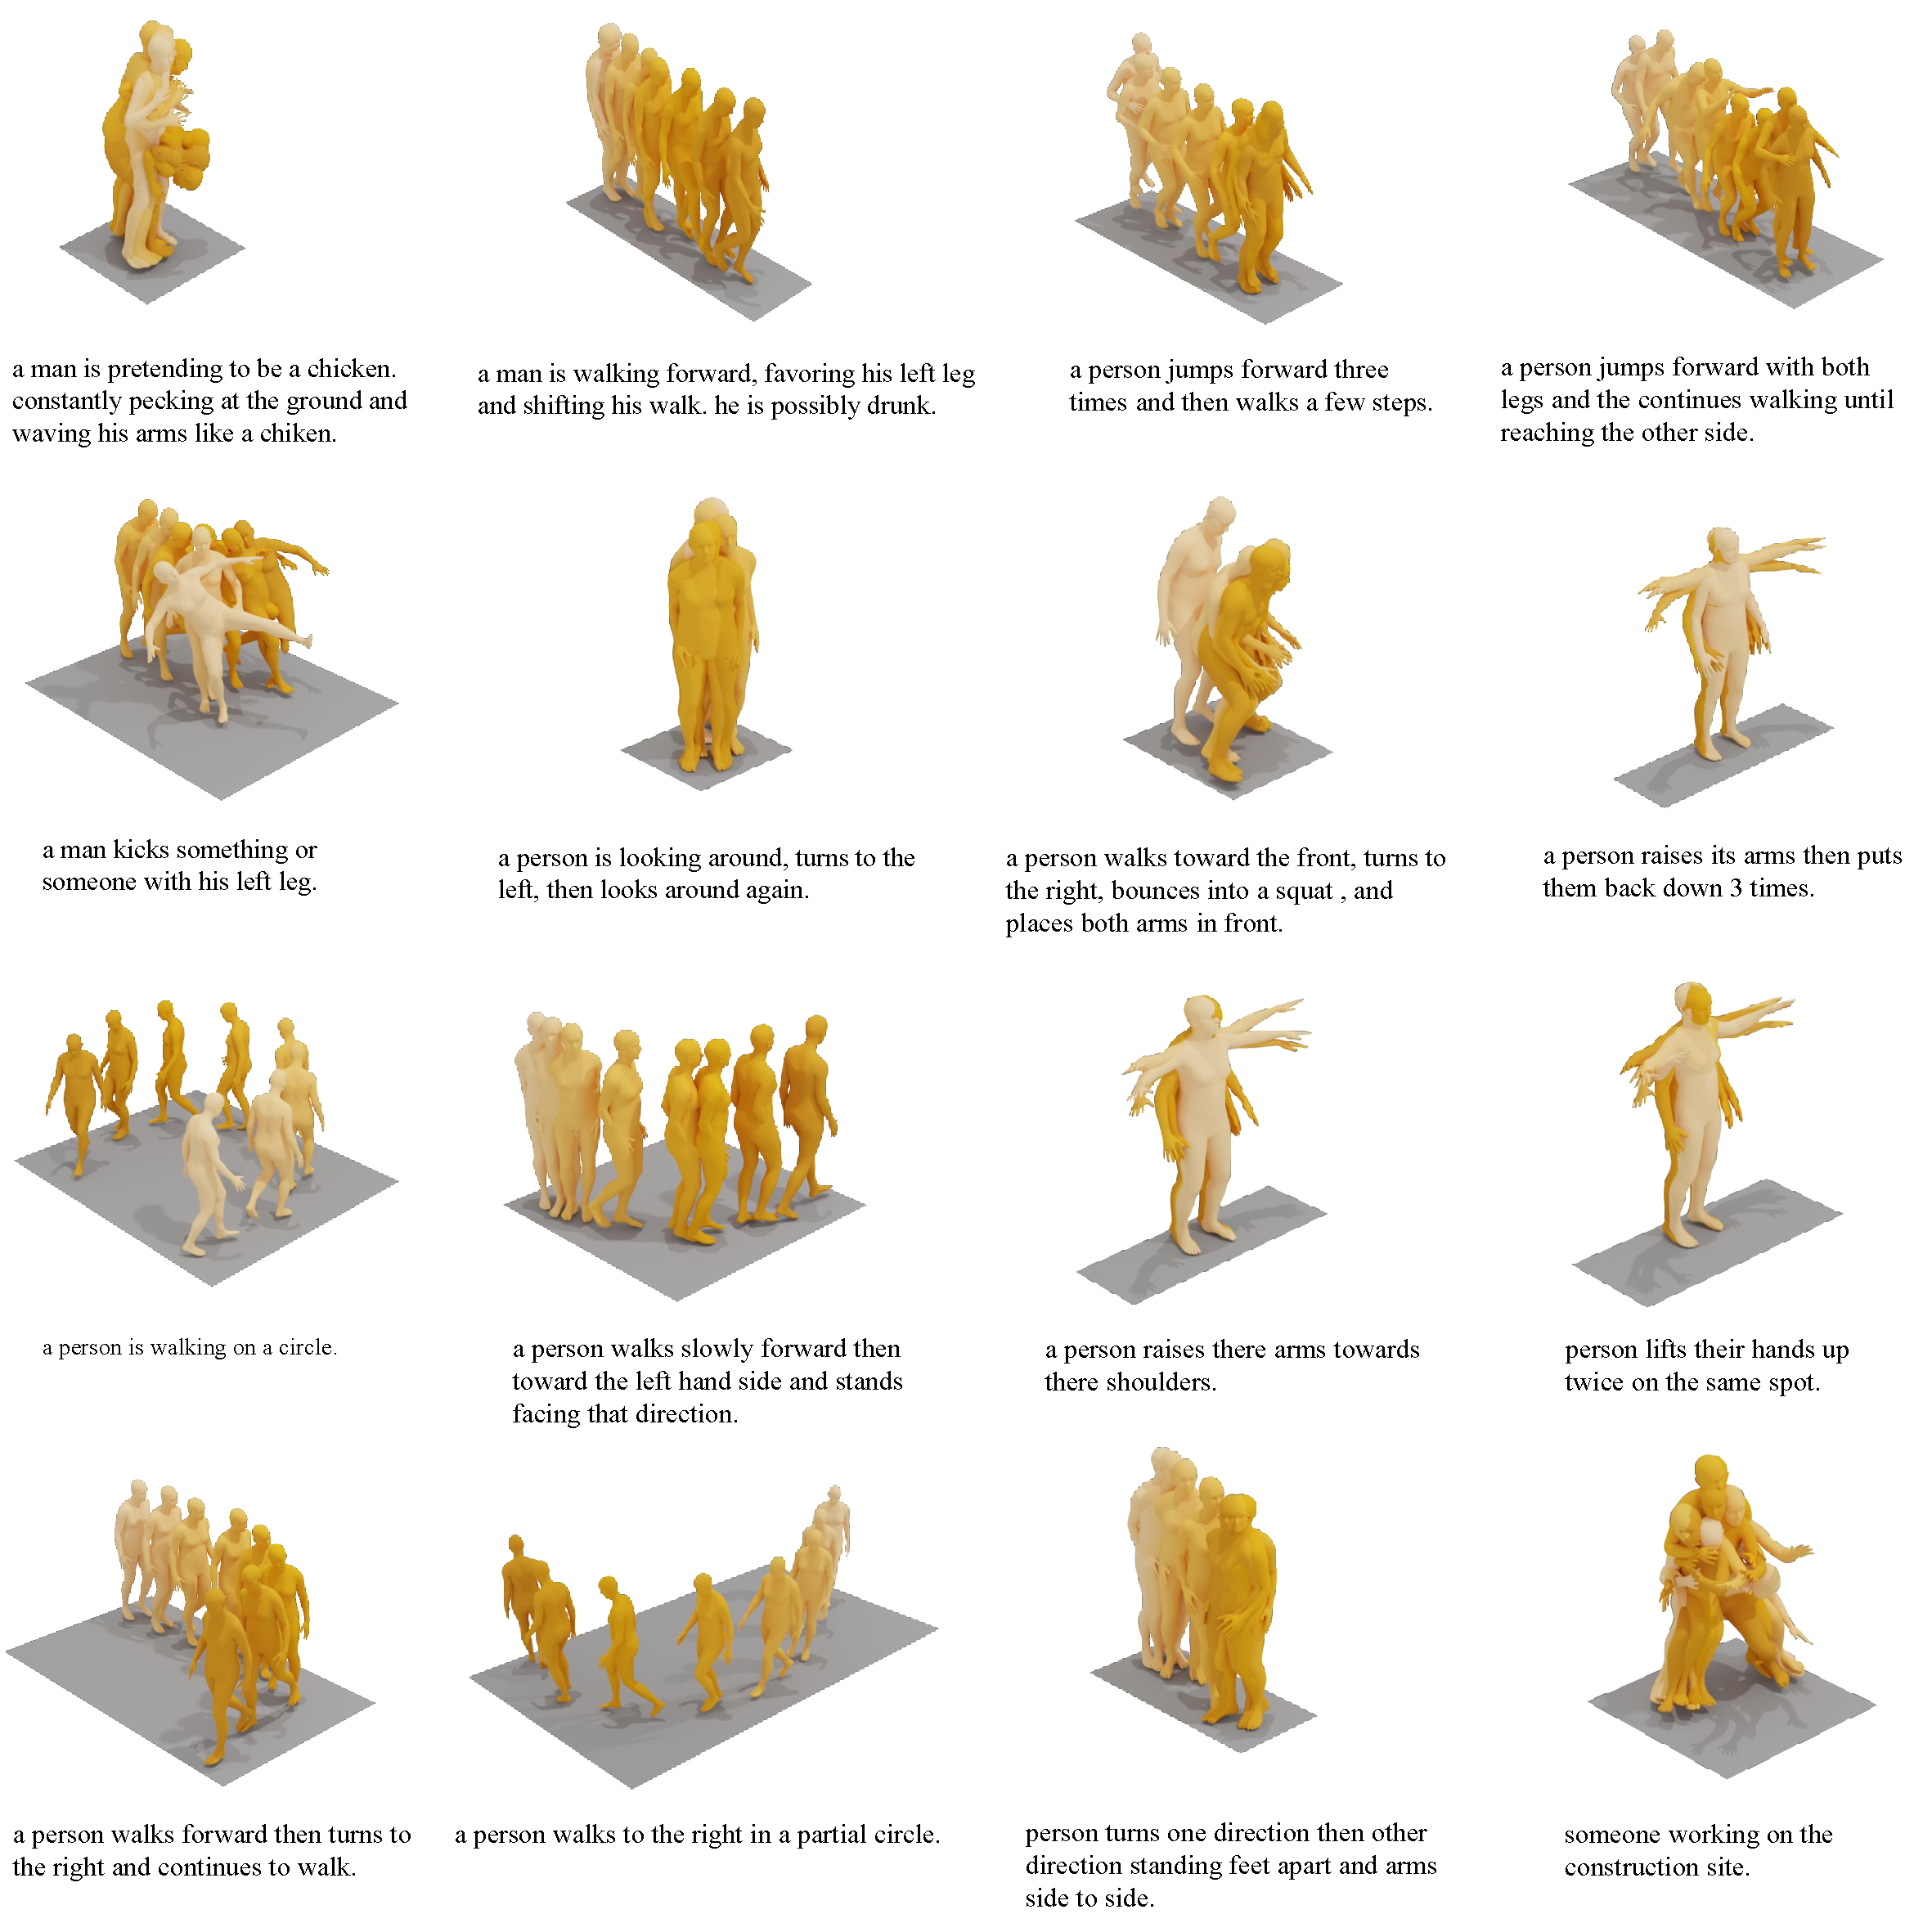
\includegraphics[width=1\linewidth]{fig/demo_00.pdf}
    \caption{
We randomly sample and visualize 16 motions generated by the proposed ReMoMask framework. These examples are conditioned on diverse prompts randomly selected from the HumanML3D~\cite{humanml3d}, providing qualitative evidence of the model’s ability to synthesize a wide range of realistic and semantically coherent motions.
    }
    \label{fig:demo}
\end{figure*}


\begin{figure*}
        \centering
    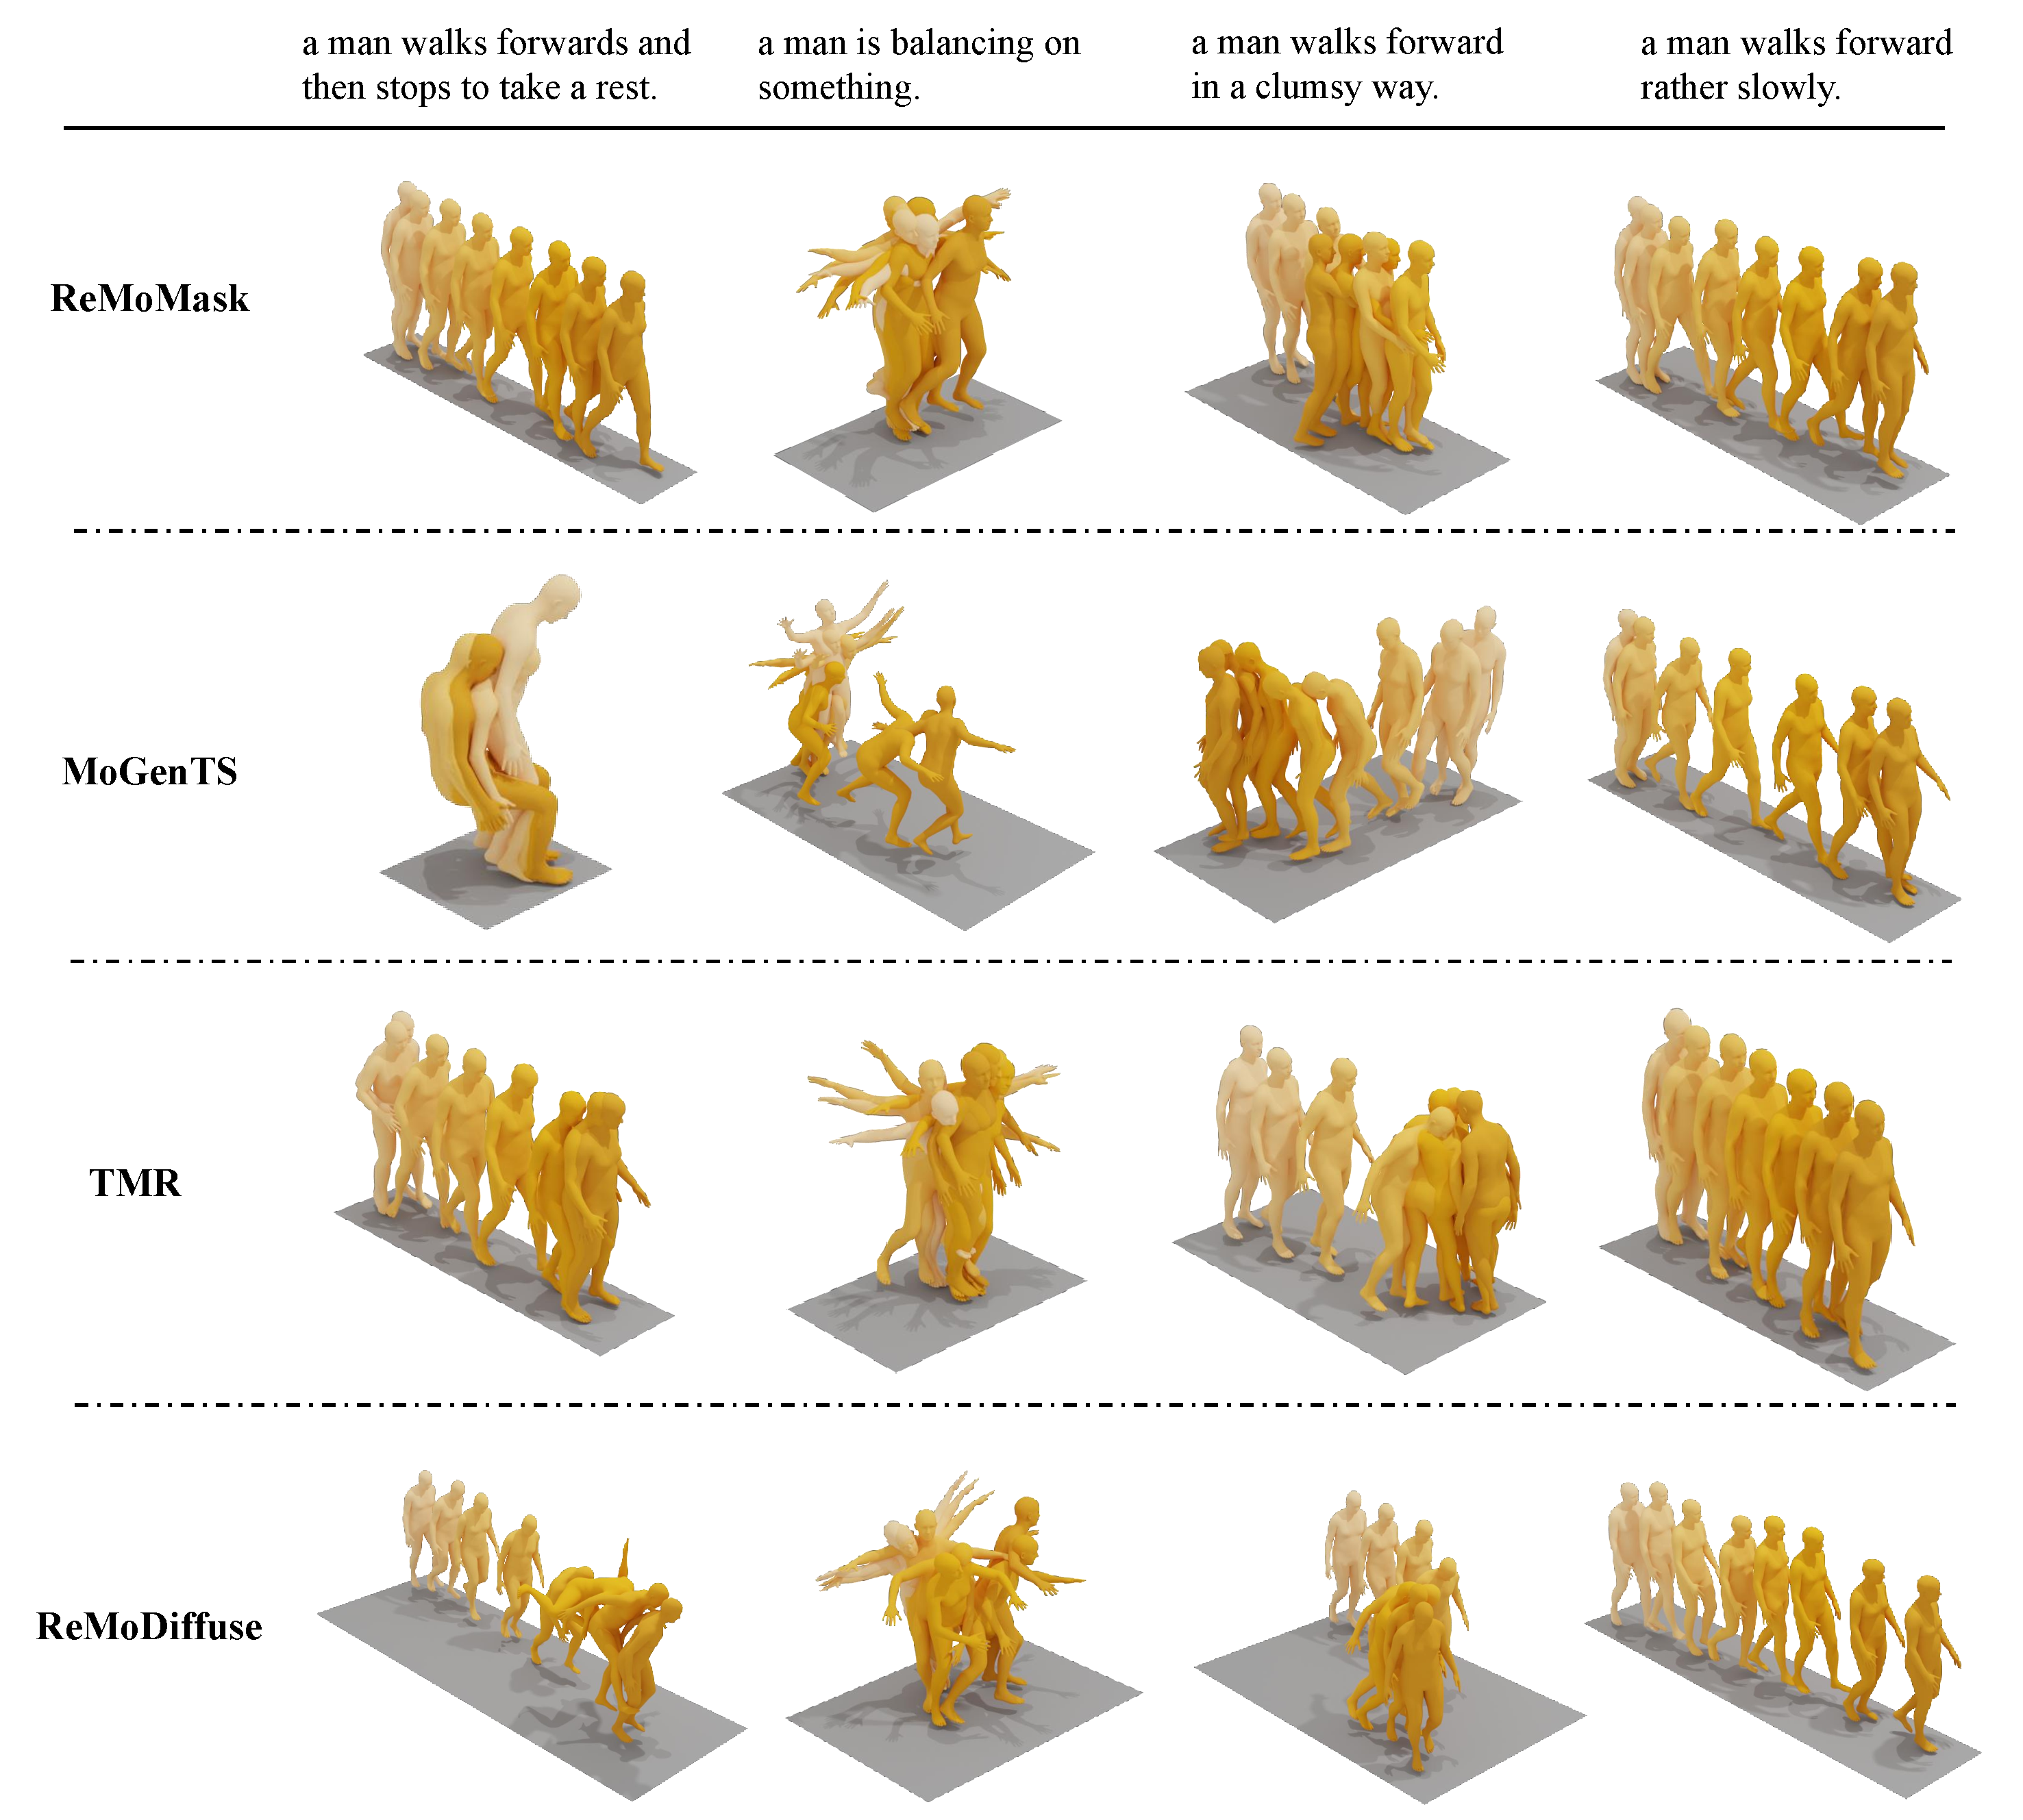
\includegraphics[width=1\linewidth]{fig/compare_00.pdf}
    \caption{
    Comparison of the proposed ReMoMask with three state-of-the-art methods: MoGenTS~\cite{mogents}, TMR~\cite{tmr}, and ReMoDiffuse~\cite{remodiffuse}. We visualize motion sequences generated in response to three distinct text prompts. Each row corresponds to a specific prompt, and each column represents the output of a different method. The results demonstrate that ReMoMask produces more realistic and semantically aligned motions compared to existing approaches.
    }
    \label{fig:demo1}
\end{figure*}


\section{Limitations}
\label{sec:limitations}
We find that the effectiveness of the proposed retrieval-augmented framework depends on the quality and coverage of the motion database. 
% When relevant motions are absent or sparsely represented in the retrieval corpus, the benefits of retrieval may be limited.
When relevant motions are absent or sparsely represented in the retrieval corpus, the framework primarily relies on its strong generative prior.
Richer motion databases remain an important direction for future work.
In addition, as quantified in Section~\ref{sec:preliminary}, the pre-quantization latent space $z_e$ is strongly anisotropic, which may bound the discriminability of cosine-based latent retrieval. Moreover, because the query projector is trained by distillation, its retrieval quality is inherently limited by the HBM teacher. Finally, retrieval in ReMoMask-2 is performed once per prompt before generation; interleaving retrieval with the iterative unmasking schedule (dynamic retrieval) is a promising direction for future work.


\section{Conclusion}
\label{sec:conclusion}

In this work, we present ReMoMask, a retrieval-augmented masked model for text-to-motion generation. To overcome the limitations of coarse-grained retrieval and ineffective fusion, we introduce \textbf{H}ierarchical \textbf{B}idirectional \textbf{M}omentum (HBM) for precise text-motion alignment and \textbf{T}opology \textbf{S}tructured \textbf{M}asking (TSM) to enforce structural consistency during training. Complemented by \textbf{S}emantic \textbf{S}patial-\textbf{T}emporal \textbf{A}ttention (SSTA) for knowledge integration, ReMoMask effectively bridges structured retrieval with high-quality generation. Extensive experiments on HumanML3D, KIT-ML, and SnapMoGen confirm that our method consistently outperforms state-of-the-art approaches in both retrieval accuracy and motion fidelity.

This article further extends ReMoMask along a third design axis, the representation consistency between the retrieval space and the generative latent space. The resulting ReMoMask-2 anchors retrieval in the pre-quantization latent space $z_e$ of the frozen RVQ-VAE, drawing text queries into this space through a small projector that inherits the HBM retriever's ranking, so evidence reaches the generator already expressed in its native representation. Latent alignment in turn removes the assumption behind the conference value-pathway design: the retrieved text embedding $R_t$ becomes a motion-domain signal and can be re-admitted into the Value pathway of SSTA. With the generative architecture otherwise unchanged, ReMoMask-2 improves generation quality over ReMoMask by \textbf{[TBD]} on HumanML3D, extending structural consistency from alignment and fusion to the underlying representation itself.

\noindent\textbf{Acknowledgements.}
This work was supported by the Fundamental Research Funds for the Central Universities, Peking University.


\appendix
\small
\section{Notations and Symbols}
\label{app:notation}
% % \begin{table}[t]
% \begin{table}[t][]
% \centering
% \caption{\textbf{Notations and symbols used in ReMoMask.}}
% \setlength{\tabcolsep}{4pt}
% \small % Adjust the font size
% % % \setlength{\tabcolsep}{3.5pt}  % Adjust the column spacing

% \renewcommand{\arraystretch}{1.1}
% \resizebox{0.75\linewidth}{!}{
%     % \begin{tabular}{l | l}
%     \begin{tabular}{p{2.2cm} | l}
%         \toprule
%             \textbf{Symbol} & \textbf{Definition} \\
%         \midrule
%             $t$ & Text prompt embedding \\
%             $z$ & Latent motion representation \\
%             $z_{1d}$ & 1D latent motion representation \\
%             $z_{2d}$ & 2D latent motion representation \\
%             $R_m$ & Retrieved motion embedding \\
%             $R_t$ & Retrieved text embedding \\
%             $E$ & Concatenated embedding of text and retrieved information \\
%             $I$ & Information embedding after projection \\
%             $K$ & Number of motion parts \\
%             $T$ & Number of temporal frames \\
%             $J$ & Number of body joints \\
%             $N$ & Length of the flattened 2D motion representation \\
%             $B$ & Batch size \\
%             $g$ & Global motion embedding \\
%             $p_{k}$ & Part-level motion embedding for the $k$-th body part \\
%             $\mathcal{Q}$ & Queue of negative embeddings for contrastive learning \\
%             $d$ & Dimension of latent space \\
%             $\tau$ & Temperature parameter in contrastive learning \\
%             $\lambda_{P}$ & Weighting coefficient for the part-level contrastive loss \\
%             $\mathrm{crossAttn}(\cdot)$ & Cross-Attention operation \\
%             $\mathrm{MLP}(\cdot)$ & Multilayer perceptron \\
%             $\mathrm{concat}(\cdot)$ & Concatenation operation \\
%             $\mathrm{flatten}(\cdot)$ & Flattening a 2D latent into a 1D sequence \\
%             % $\mathcal\begin{table}retrieval database \\
%             % $\mathcal{L}_{\text{HBM}}$ & Hierarchical bidirectional Momentum Contrastive Learning loss \\
%         \bottomrule
%     \end{tabular}
% }
% \label\end{table}n}
% \end{table}



\begin{table}[t]
\centering
\caption{\textbf{Notations and symbols used in ReMoMask and ReMoMask-2.}}
\setlength{\tabcolsep}{4pt}
\small
\renewcommand{\arraystretch}{1.1}
\resizebox{\linewidth}{!}{
\begin{tabular}{p{2.2cm} | l}
\toprule
\textbf{Symbol} & \textbf{Definition} \\
\midrule

$x$ & Input text prompt \\

$m$ & Motion sequence \\

$m^k$ & Motion of the $k$-th body part \\

$t_i$ & Text embedding of the $i$-th sample \\

$g_i$ & Global motion embedding \\

$p_{i,k}$ & Part-level motion embedding for the $k$-th body part \\

$R_m$ & Retrieved motion embedding \\

$R_t$ & Retrieved text embedding \\

$z$ & Latent motion tokens arranged on a $T \times J$ spatial--temporal grid \\

$z_{\mathrm{pred}}$ & Reconstructed latent motion tokens predicted by the generator \\

$h_{\mathrm{sem}}$ & Global semantic token constructed from text and retrieved context \\

$Q,K,V$ & Query, Key, and Value matrices in the attention module \\

$\alpha_{i,k}$ & Semantic relevance between text and the $k$-th body part \\

$\pi_{\mathrm{base}}$ & Base masking probability \\

$\pi_{i,k}$ & Masking probability of the $k$-th body part \\

$\mathcal{Q}$ & Momentum queue storing negative embeddings \\

$\mu$ & Momentum coefficient for updating momentum encoders \\

$\tau$ & Temperature parameter in contrastive learning \\

$\lambda_{P}$ & Weighting coefficient for the part-level contrastive loss \\

$B$ & Batch size \\

$K$ & Number of body parts \\

$T$ & Number of temporal frames \\

$J$ & Number of body joints \\

$N$ & Length of flattened motion tokens ($N=T \times J$) \\

$d$ & Dimension of the latent embedding space \\

$\mathrm{MLP}(\cdot)$ & Multilayer perceptron \\

$\mathrm{concat}(\cdot)$ & Concatenation operation \\

$\mathrm{flatten}(\cdot)$ & Flattening a 2D latent grid into a 1D sequence \\

\midrule

$\mathcal{S}$, $\mathcal{Z}$ & Contrastive semantic space; generative latent space \\

$\psi$ & Implicit cross-space translation $\mathcal{S} \rightarrow \mathcal{Z}$ in ReMoMask \\

$z_e$ & Pre-quantization continuous latent of the frozen RVQ-VAE encoder \\

$\bar{z}_e$ & Pooled, $\ell_2$-normalized $z_e$ used as a retrieval key ($d_e$-dim.) \\

$d_e$ & Channel dimension of $z_e$ ($d_e = 1024$) \\

$\mathcal{D}$ & Latent-aligned retrieval database of $(\bar{z}_e, x)$ pairs \\

$\phi$ & Query projector mapping CLIP text embeddings into the $z_e$ space \\

$\kappa$ & Number of teacher candidates in distillation (top-$\kappa$) \\

$p^{\mathrm{HBM}}, p^{\phi}$ & Teacher / student retrieval distributions in KL distillation \\

\bottomrule
\end{tabular}
}
\label{tab:notation}
\end{table}

We list notations and symbols used in this paper, as shown in Table~\ref{tab:notation}.



% \input{appendix/sec/relatedwork}

% \section{Metrics}
% \label{app:metrics}
\section{User Study}
\label{sec:userstudy}

To comprehensively evaluate the generation capability of \textbf{ReMoMask}, we conducted a comparative user study.  
We randomly selected 20 text prompts from the HumanML3D test set and generated motion sequences using \textbf{ReMoMask}, current state-of-the-art retrieval-augmented method (ReMoDiffuse), generative model (MoMask), and ground truth motions.  


We employ a forced-choice paradigm in our user study, asking participants two key questions: “Which of the two motions is more realistic?” and “Which of the two motions corresponds better to the text prompt?”. The study is conducted via a Google Forms interface, as illustrated in Fig.~\ref{fig:UI}. To ensure fairness and reduce potential bias, the names of the generative models are hidden, and the order of presentation is randomized for each question. In total, over 50 participants took part in the evaluation.

Empirical results, depicted in Fig.~\ref{fig:picture1} and Fig.~\ref{fig:picture2}, underscore ReMoMask’s strong capability to generate motions that are not only realistic but also closely aligned with textual descriptions. Specifically, as shown in Fig.~\ref{fig:picture1}, ReMoMask achieves a 42\% preference rate over ground truth (GT) in terms of realism. Although GT motions are derived from real human data, this result indicates that ReMoMask is perceived as comparably realistic by human evaluators. Moreover, the model significantly outperforms both baselines: it achieves 67\% preference over MoMask and 75\% over ReMoDiffuse, demonstrating its strength in producing high-quality, lifelike motion sequences.

In terms of text correspondence (reported in Fig.~\ref{fig:picture2}), ReMoMask attains a 47\% preference rate over GT, suggesting that its generated motions exhibit nearly human-level alignment with text prompts. Compared to the baselines, ReMoMask again shows substantial improvements, with 72\% preference over MoMask and 86\% over ReMoDiffuse.



\begin{figure}[h]
    \centering
    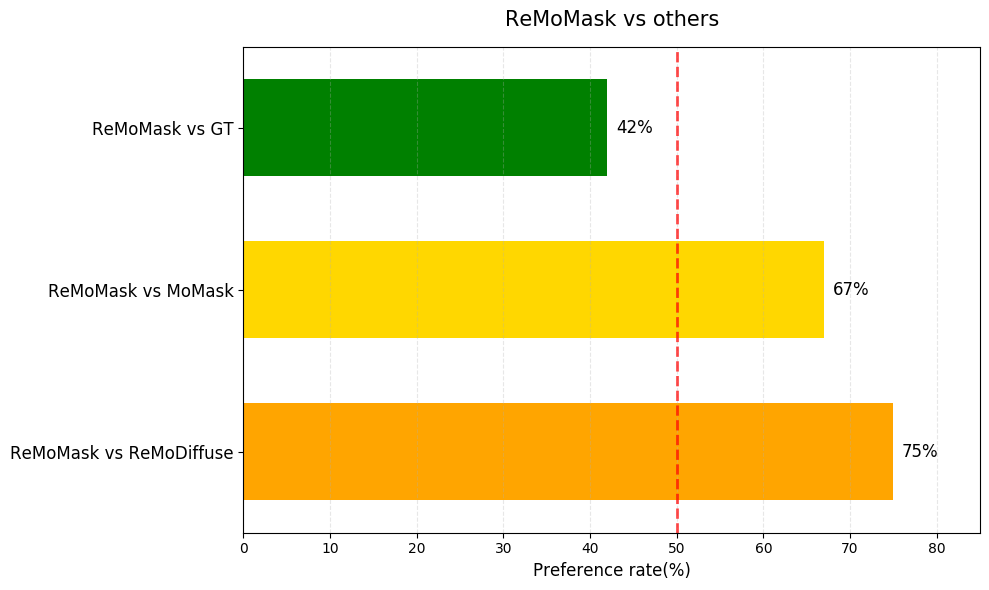
\includegraphics[width=\linewidth]{fig/question_2.png}
    \caption{
      Motion Quality User Study
    }
    \label{fig:picture1}
\end{figure}

\begin{figure}[h]
    \centering
    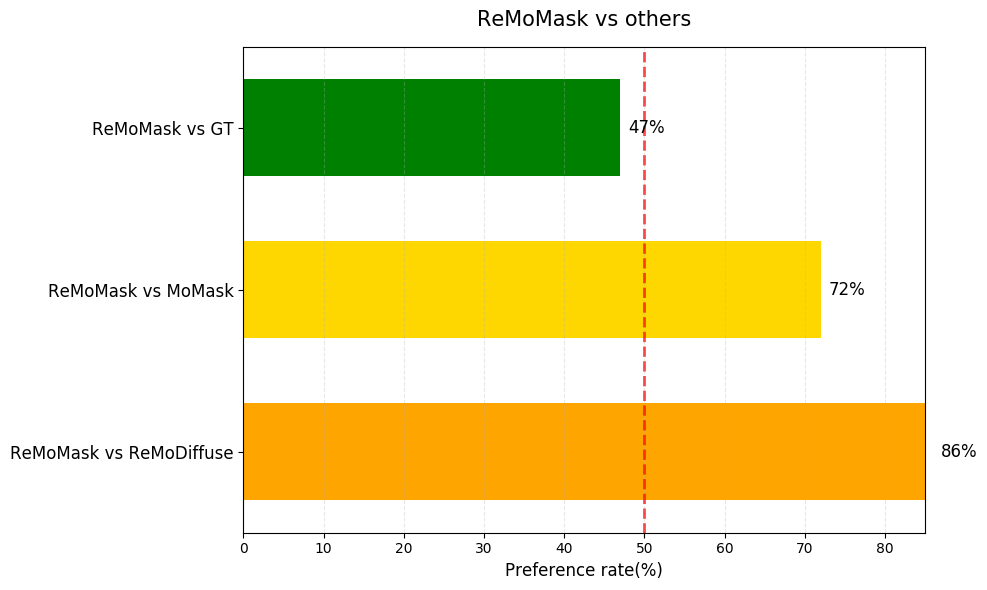
\includegraphics[width=\linewidth]{fig/question_1.png}
    \caption{
    Text-Motion Correspondence User Study
    }
    \label{fig:picture2}
\end{figure}





\textbf{Video Demonstrations.}
We provide video demonstrations of our generated motions to facilitate qualitative evaluation. Fig.~\ref{fig:video_sample} shows representative video samples, where our method produces temporally coherent and semantically aligned motion sequences.

\begin{figure}[t]
    \centering
    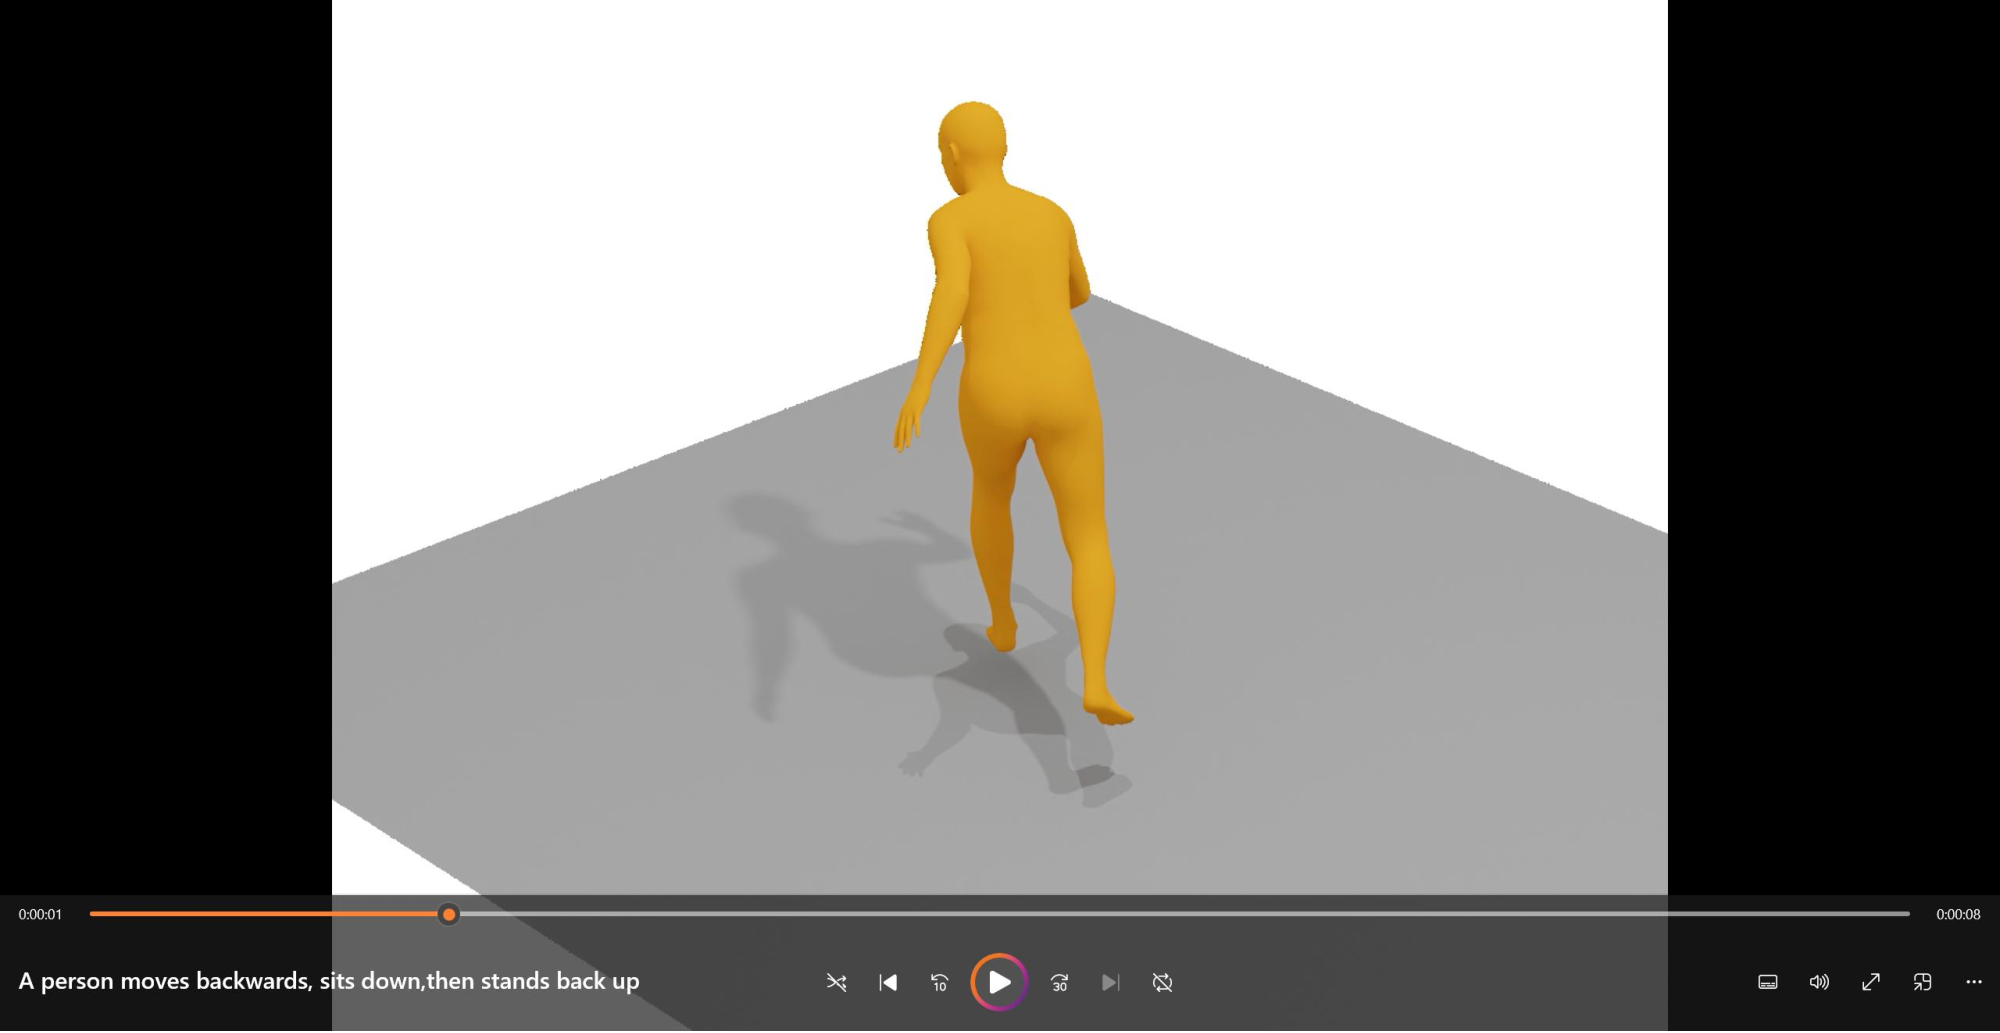
\includegraphics[width=0.80\linewidth]{fig/rebuttal_video.pdf}
    \vspace{-10pt}
    \caption{Video sample.}
    \vspace{-10pt}
    \label{fig:video_sample}
\end{figure}


\begin{figure*}
        \centering
    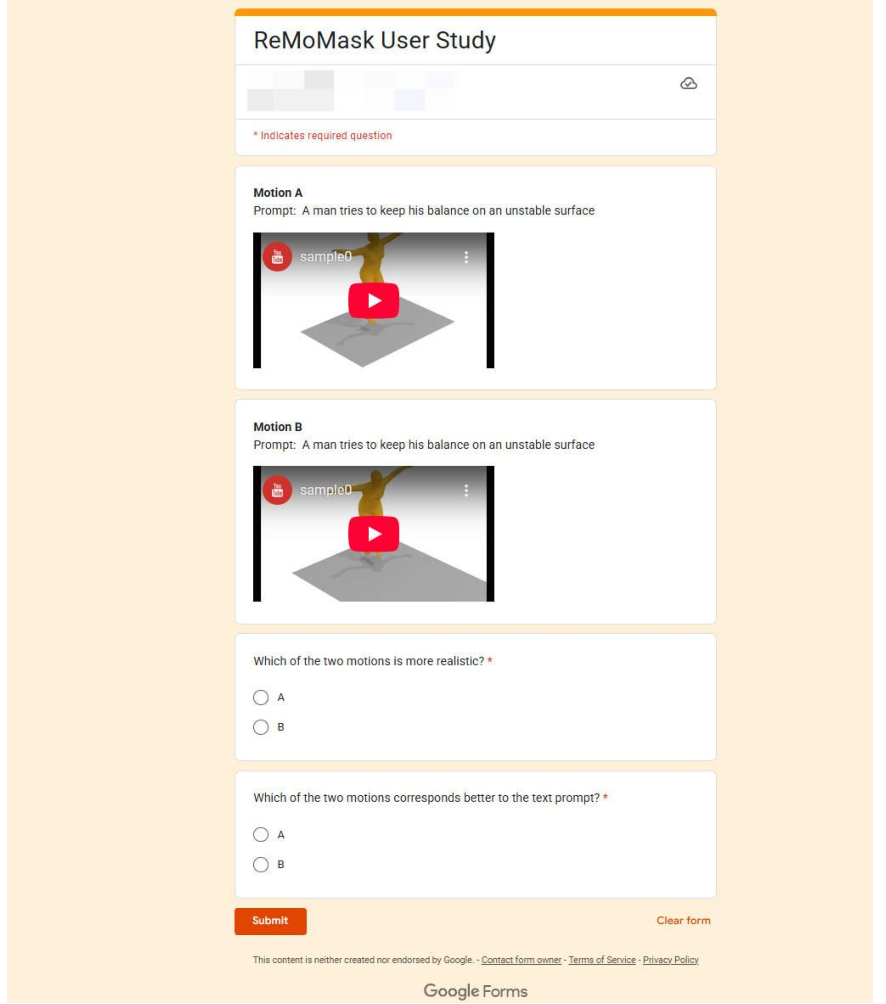
\includegraphics[width=1\linewidth]{fig/userStudy.pdf}
    \caption{
    This figure illustrates the User Interface (UI) used in the ReMoMask User Study. Participants are presented with two motion videos, labeled as Motion A and Motion B, alongside a shared textual prompt. The motion clips are sampled from outputs generated by different models or the ground truth (GT), with model identities anonymized and video order randomized. Participants are asked to answer two evaluative questions: (1) “Which of the two motions is more realistic?”, assessing the visual plausibility and motion quality; and (2) “Which of the two motions corresponds better to the text prompt?”, evaluating the semantic alignment between the motion and the given description. This dual-question design enables a comprehensive human assessment of both motion realism and text-motion correspondence.
    }
    \label{fig:UI}
\end{figure*}
\clearpage
\bibliographystyle{IEEEtran}
\bibliography{reference}


% biography section
%% 
%% If you have an EPS/PDF photo (graphicx package needed) extra braces are
%% needed around the contents of the optional argument to biography to prevent
%% the LaTeX parser from getting confused when it sees the complicated
%% \includegraphics command within an optional argument. (You could create
%% your own custom macro containing the \includegraphics command to make things
%% simpler here.)
%%\begin{IEEEbiography}[{\includegraphics[width=1in,height=1.25in,clip,keepaspectratio]{mshell}}]{Michael Shell}
%% or if you just want to reserve a space for a photo:
%
%\begin{IEEEbiography}{Michael Shell}
%Biography text here.
%\end{IEEEbiography}
%
%% if you will not have a photo at all:
%\begin{IEEEbiographynophoto}{John Doe}
%Biography text here.
%\end{IEEEbiographynophoto}
%
%% insert where needed to balance the two columns on the last page with
%% biographies
%%\newpage
%
%\begin{IEEEbiographynophoto}{Jane Doe}
%Biography text here.
%\end{IEEEbiographynophoto}

% biography section

\begin{IEEEbiography}[{
\includegraphics[width=1in]{Figures/zeyu.jpeg}}]{Zeyu Zhang}
is an incoming PhD student at UC Berkeley BAIR, advised by Prof. Pieter Abbeel, Prof. Alexei A. Efros, and Prof. Angjoo Kanazawa. He received his bachelor's degree from the Australian National University, where he was advised by Prof. Richard Hartley and Prof. Ian Reid. His research interests lie in geometric generative modeling and its applications to world models, multimodal foundation models, embodied AI, and AI for health. 
\end{IEEEbiography}


\begin{IEEEbiography}[{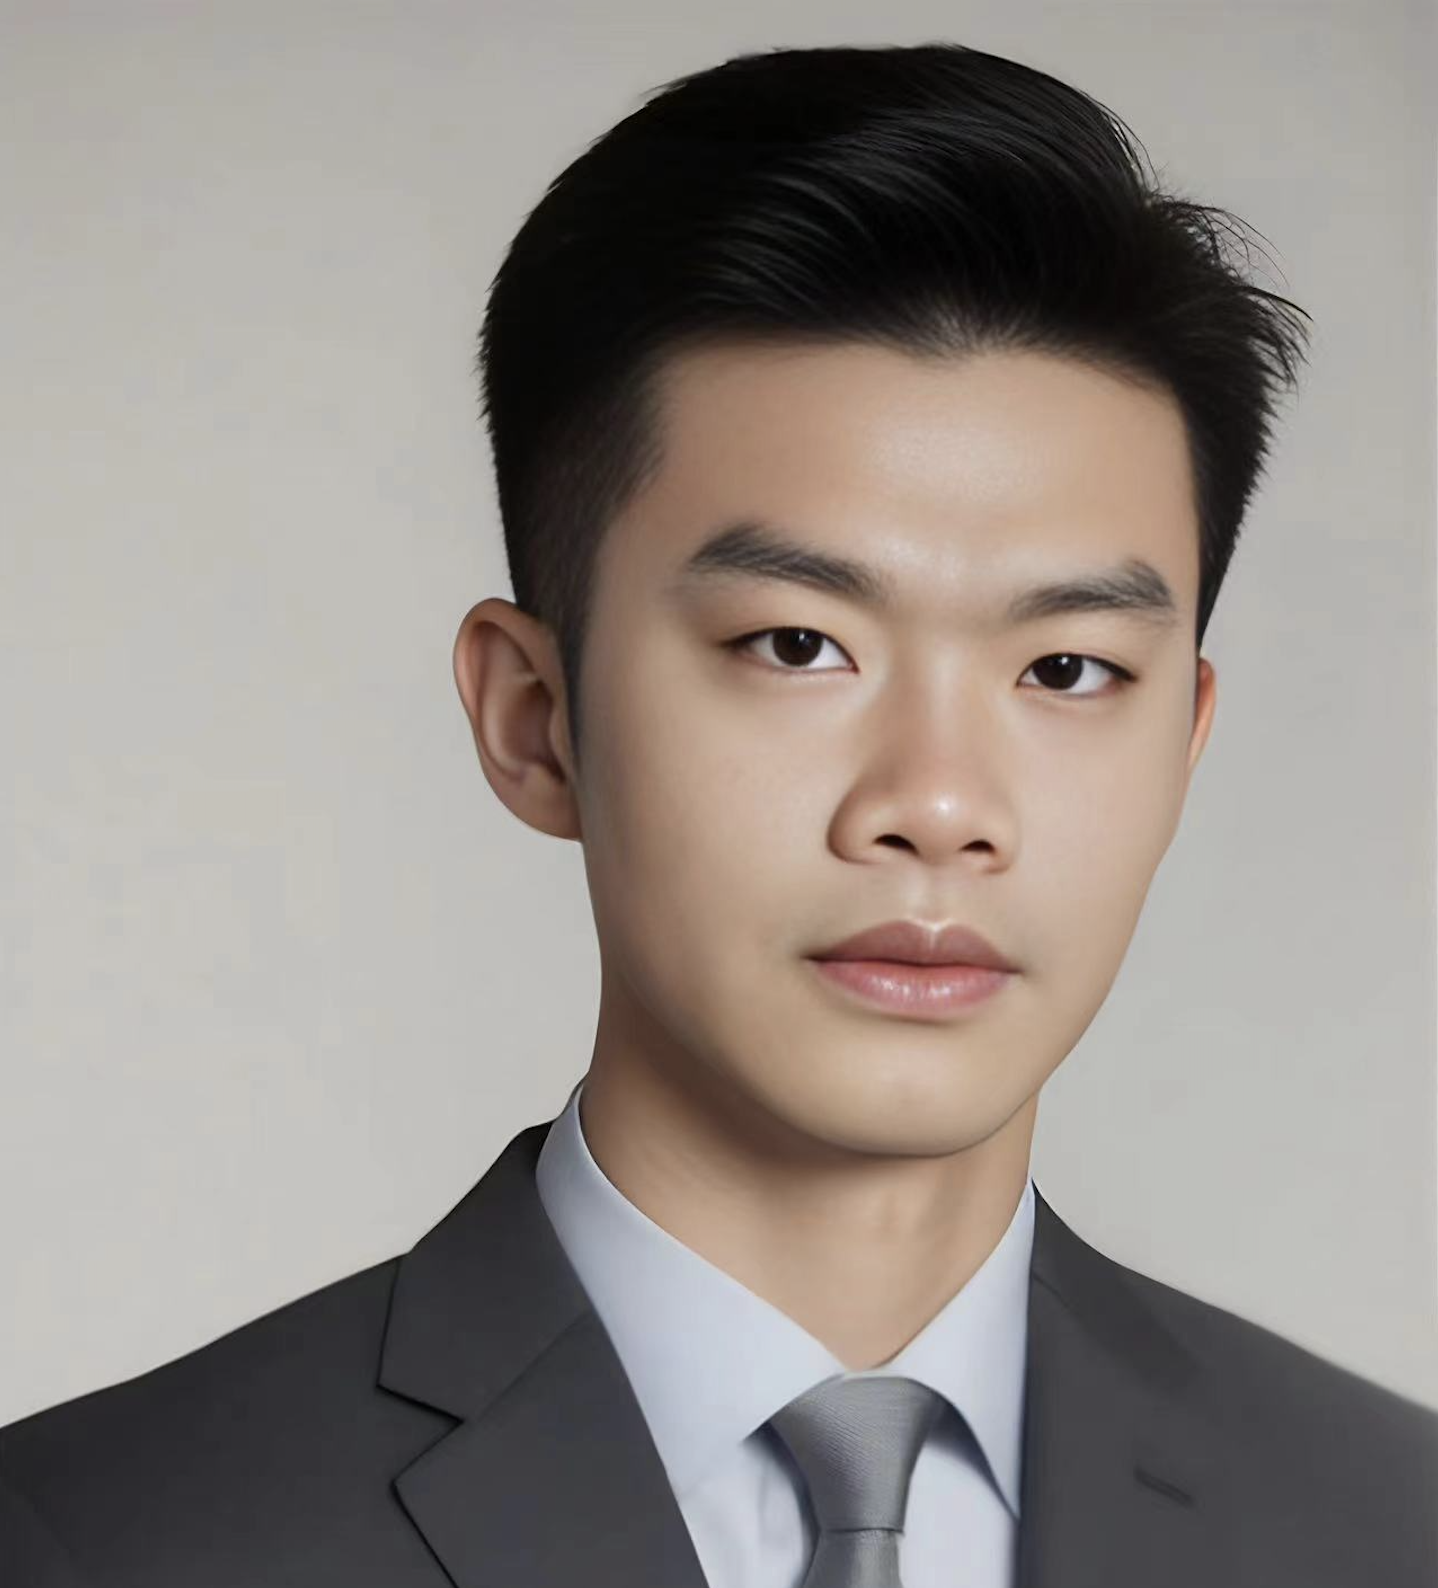
\includegraphics[width=1in,height=1.25in,clip,keepaspectratio]{Figures/HT.png}}]{Hao Tang}
is an Assistant Professor at Peking University, China. Previously, he held postdoctoral positions at CMU, USA, and ETH Zürich, Switzerland. He earned his master’s degree from Peking University, and his Ph.D. from the University of Trento, Italy.
He has had the opportunity to visit the University of Oxford, Northeastern University, NUS, and IIAI, among other institutions.
His research interests include computer vision, embodied AI, and generative AI, as well as their applications in scientific domains.
\end{IEEEbiography}






% You can push biographies down or up by placing
% a \vfill before or after them. The appropriate
% use of \vfill depends on what kind of text is
% on the last page and whether or not the columns
% are being equalized.

%\vfill

% Can be used to pull up biographies so that the bottom of the last one
% is flush with the other column.
%\enlargethispage{-5in}

% that's all folks





\end{document}